

%\chapter{Entity-Based Models}
\label{chapt:entity_based_models}
%
The coherence of a text is interpreted by means of relations, including both explicit and implicit, among sentences of a text. 
Various types of relations may exist between sentences. 
Entity-based relations are taken as a major relation type because entities are a prominent information for NLP applications (e.g., question answering) and information retrieval systems. 
So it is required to have a definition of an entity.
We refer to an entity as a person, an object or abstraction that exists (or could exist) external world to the text. 
Entities have been extracted as important information in Information Extraction (IE) applications. 
For instance, in entity disambiguation -- as a well-known task in IE -- the goal is to extract word spans that refer to either a person, organization, time, and etc. 
Pieces of a text that we use to refer to an entity are named mentions. 
Entity can be referred to in various ways by mentions. 
It turns out that identifying mentions that refer to the same entity in a text contributes to the IE tasks. 
This task is known as coreference resolution in that the goal is to cluster mentions of a text based on entities that they are referring to.  
Each cluster, which can be imagined as a bucket containing all referent mentions, represent an entity. 
In practice, mentions of an entity are linked together in order to show that they are referring to the same entity. 
Since in IE entities are part of the important information in texts, connections between mentions not only show that those are referring to the same entity, but also indicate this fact that sentences that contain those mentions are almost about the same topic or information. 
This fact is the basis of entity-based coherence models: sentences that contain mentions of an entity are related. 
The way entities are mentioned, distributed, among sentences of a text represents certain regularities in well-written texts form that distinguish other texts. 
Well-written texts are coherent because the relations between sentences, which are based on the relation between mentions of entities in entity-based models, make texts more semantically interpretable. 


Coherent texts focus on a few important entities, where entities and their interactions are easy-to-understand.  
The main intuition of the entity-based models is that texts fraught with abrupt switches from one topic to the another require a long time for realizing the relations between topics. 
The patterned distribution of discourse entities is a natural consequence of topic continuity observed in a coherent text. 

Linguistically point of view, Centering Theory \cite{grosz95} is the most inspiring theory for entity-based models.  
Centering Theory formulates fluctuations in topic continuity with regard to transitions between adjacent sentences 
\footnote{Centering Theory defines transitions over utterances, we simplify it as sentences.}.
Texts manifesting particular types of transitions, or patterns, are perceived more coherent than texts where such transitions are absent or sparse. For example, CONTINUE transitions require that two sentences share at least one entity and are preferred
over transitions that frequently SHIFT from one entity to the other. 

Entity-based models are building blocks for our models and contributions in the rest of this thesis. 
Therefore, in this chapter, we explain details of two well-known entity-based coherence models: Entity Grid and Entity Graph models. 
Then we propose an improved version of the Entity Graph model.  
We report the results of these models on sentence ordering, summary coherence rating, and readability assessment as three benchmark tasks for coherence evaluation; explaining that our improved model of Entity Graph outperforms the other two models on these examined tasks. 
This chapter covers the pros and cons of each of the mentioned models and motives the application of graph-based framework in text representation for the rest of the thesis. 


\section{The Entity Grid Model}
\label{sec:ent_grid}
%
\newcite{barzilay05a,barzilay08} were the first researchers who proposed a computationally coherence model based on the entity relations among sentences. 
In this thesis, we refer to their model as the Entity Grid model,  
because the key idea of this model is to represent a text as a grid that captures patterns of entity distribution across sentences of a text. 
supported by some linguistic work such as Centering Theory \cite{grosz95} and other entity-based theories of discourse \cite{givon87,prince81a}, they assume that the distribution of entities in locally coherent texts exhibits certain regularities that can be reflected in a grid topology that is called entity grid.

With respect to Centering Theory, coherence can be measured by predicting both repetitions of important entities in adjacent sentences, and also the syntactic forms and positions of mentions to those entities. 
In order to find the important entities, Centering Theory retains the track of a ranked list of entities in each sentence, from which the most salient mention of the next sentence is identified. 
The ranking depends on syntactic role (for instance, the subject of a sentence is more prominent than the object of a preposition), but also on other syntactic cues and on the current context of entities. 
Motivated by this, \newcite{barzilay05a,barzilay08} define all possible grammatical transitions of entities in a text as a possible coherence patterns that coherence is encoded by the frequency of these patterns.


\subsection{Text Representation: Entity Grid}
%
An entity grid represents a text as a two dimensional array whose columns correspond to entities, and rows are matching to sentences.
The entry $r_{i;j}$ describes the syntactic role of entity $j$ in sentence $i$ if the entity is mentioned in the sentence. 
The syntactic roles are categorized as subject (S), object (O), or all other syntactic role (X). 
In addition, if an entity is not mentioned in a sentence a special marker (-) fills the corresponding entry of the entity grid. 
In contrast, if a sentences contains different mentions of an entity, its grid symbol describes the most important of its grammatical roles: subject if possible, then object, or finally other. 


This discussion of the grid develops around the important question of which textual units are to be considered mentions of an entities, and how different mentions are to be linked to represent an entity.
A perfect solution in this regard would use coreference resolution to recognize mentions, noun phrases, and link arbitrary mentions to the same entities and discarding noun phrases which do not correspond to an entity. 
Since coreference resolution systems are far from prefect, and tend to work even more poorly on incoherent texts, this approach is not generally one utilized. 
It turns out a poor coreference system introduces more errors to coherence model than what it fixes \cite{barzilay05}.
As an alternative, implementations of the entity grid tend to employ all noun phrases as mentions and perform heuristic, but strict and simple, coreference resolution by connecting mentions that have an identical head noun as an entity. 
Detailed discussions of this heuristic are given in \newcite{poesio04c} and \newcite{elsner10}.

Here is a sample text from DUC dataset (more explanation in Section \ref{}) and its entity grid representation.

\begin{table}
\centering
\begin{tabular}{l@{\space}p{15cm}} %p@{\linewidth}
\hline
 $S_0$: & [An arctic cold wave]\textbf{\textsubscript{S}}, [the worst]\textbf{\textsubscript{X}} in [10 years]\textbf{\textsubscript{X}}, hit [parts]\textbf{\textsubscript{O}} of [Europe]\textbf{\textsubscript{X}}, bringing [sub-zero temperatures]\textbf{\textsubscript{O}} and killing [scores]\textbf{\textsubscript{O}} of [people]\textbf{\textsubscript{X}}. \\

 $S_1$: & Hardest hit were [Poland]\textbf{\textsubscript{S}}, [Bulgaria]\textbf{\textsubscript{S}}, and [Romania]\textbf{\textsubscript{S}} as well as [parts]\textbf{\textsubscript{S}} of [central]\textbf{\textsubscript{X}} and [eastern France]\textbf{\textsubscript{X}}. \\

$S_2$: & In [Poland]\textbf{\textsubscript{X}}, [three weeks]\textbf{\textsubscript{X}} of [sub-zero temperatures]\textbf{\textsubscript{X}} killed [at least 85 people]\textbf{\textsubscript{O}} in [November]\textbf{\textsubscript{X}}, 29 more than in [all]\textbf{\textsubscript{X}} of [the previous winter]\textbf{\textsubscript{S}}. \\


$S_3$ : & [Most]\textbf{\textsubscript{S}} of [the victims]\textbf{\textsubscript{X}} were homeless [whose deaths]\textbf{\textsubscript{X}} by [exposure]\textbf{\textsubscript{X}} were alcohol related. \\

$S_4$: & [Blizzards]\textbf{\textsubscript{X}} and [cold temperatures]\textbf{\textsubscript{S}} also hit [Bulgaria]\textbf{\textsubscript{X}} and [Romania]\textbf{\textsubscript{O}}, stranding [hundreds]\textbf{\textsubscript{O}} in [their cars]\textbf{\textsubscript{X}}. \\

$S_5$: & Elsewhere, [snow]\textbf{\textsubscript{S}} blanketed [the Italian island]\textbf{\textsubscript{O}} of [Capri]\textbf{\textsubscript{X}} for [the first time]\textbf{\textsubscript{X}} in [10 years]\textbf{\textsubscript{X}}.  \\


\hline
\end{tabular}
\caption{/hits/fast/nlp/mesgarmn/Data/ACL13/SummaryCoherence/texts/D31010.M.100.T.E.txt. Nubembers (e.g. 29) are filtered out in preprocessing.}
\end{table}

%%(ROOT (S (NP (NP (DT An) (JJ arctic) (JJ cold) (NN wave)) (, ,) (NP (NP (DT the) (JJS worst)) (PP (IN in) (NP (CD 10) (NNS years)))) (, ,)) (VP (VBD hit) (NP (NP (NNS parts)) (PP (IN of) (NP (NNP Europe)))) (, ,) (S (VP (VP (VBG bringing) (NP (JJ sub-zero) (NNS temperatures))) (CC and) (VP (VBG killing) (NP (NP (NNS scores)) (PP (IN of) (NP (NNS people)))))))) (. .)))

%%(ROOT (S (S (VP (ADVP (RBS Hardest)) (VBN hit))) (VP (VBD were) (NP (NP (NP (NNP Poland)) (, ,) (NP (NNP Bulgaria)) (, ,) (CC and) (NP (NNP Romania))) (CONJP (RB as) (RB well) (IN as)) (NP (NP (NNS parts)) (PP (IN of) (NP (NP (JJ central)) (CC and) (NP (JJ eastern) (NNP France))))))) (. .)))

%%(ROOT (S (PP (IN In) (NP (NNP Poland))) (, ,) (NP (NP (CD three) (NNS weeks)) (PP (IN of) (NP (JJ sub-zero) (NNS temperatures)))) (VP (VBD killed) (NP (QP (IN at) (JJS least) (CD 85)) (NNS people)) (PP (IN in) (NP (NNP November))) (, ,) (PP (ADVP (NP (CD 29)) (RBR more)) (IN than) (IN in) (NP (NP (DT all)) (PP (IN of) (NP (DT the) (JJ previous) (NN winter)))))) (. .)))

%%(ROOT (S (NP (NP (JJS Most)) (PP (IN of) (NP (DT the) (NNS victims)))) (VP (VBD were) (ADJP (JJ homeless) (SBAR (WHNP (NP (WP$ whose) (NNS deaths)) (PP (IN by) (NP (NN exposure)))) (S (VP (VBD were) (ADJP (RB alcohol) (VBN related))))))) (. .)))

%%(ROOT (S (NP (NP (NNS Blizzards)) (CC and) (NP (JJ cold) (NNS temperatures))) (ADVP (RB also)) (VP (VBD hit) (NP (NNP Bulgaria) (CC and) (NNP Romania)) (, ,) (S (VP (VBG stranding) (NP (NNS hundreds)) (PP (IN in) (NP (PRP$ their) (NNS cars)))))) (. .)))

%%(ROOT (S (ADVP (RB Elsewhere)) (, ,) (NP (NN snow)) (VP (VBD blanketed) (NP (NP (DT the) (JJ Italian) (NN island)) (PP (IN of) (NP (NNP Capri)))) (PP (IN for) (NP (NP (DT the) (JJ first) (NN time)) (PP (IN in) (NP (CD 10) (NNS years)))))) (. .)))
%%


\begin{table}
\centering
\begin{tabular}{lcccccc}
\hline
WAVE & S & - & - & - & - & - \\
WORST & X & - & - & - & -  &- \\
YEARS  &X  & -  &-  &-  &-  &X \\
PARTS  &O & S  &-  &-  &-  &-  \\
EUROPE  &X & - & - & - & - & - \\
TEMPERATURES  &O  &-  &X  &-  &S  &-  \\
SCORES  &O  &-  &-  &-  &-  &-  \\
PEOPLE  &X  &- & O  &-  &-  &-  \\
POLAND  &-  &S & X  &-  & -  &-  \\
BULGARIA  &-  &S  &-  &-  &X  &-  \\
ROMANIA  &-  &S  &-  &-  &O  &-  \\
CENTRAL  &-  &X  &- & - & - & -  \\
FRANCE  &-  &X  &-  &- & - & -  \\
NOVEMBER  &-  &- & X  &-  &-  &-  \\
WEEKS  &-  &-  &S  &-  &-  &-  \\
ALL  &-  &-  &X  &-  &-  &-  \\
WINTER  &-  & -  &X  &-  &-  &-  \\
MOST  &-  &-  &-  &S  &- & -  \\
VICTIMS  &-  &-  &-  &X  &-  &-  \\
DEATHS  &-  &-  &- & X  &-  &-  \\
EXPOSURE  &- & - & -  &X  &-  &-  \\
ALCOHOL  &-  &-  &-  &X  &-  &-  \\
BLIZZARDS  &-  &-  &-  &-  &X  &-  \\
HUNDREDS  &-  &-  &-  &-  &O  & -  \\
CARS  &-  &-  &-  &-  &X  &-  \\
TIME  &-  &-  &-  &-  &-  &X  \\
SNOW  &-  &- & - & - & - & S  \\
ISLAND & - & - & - & - & - & O  \\
CAPRI & - & - & - & - & - & X  \\
\hline
\end{tabular}
\caption{/hits/fast/nlp/mesgarmn/Data/ACL13/SummaryCoherence/NounGrid/SCR/wo\_coref/D31010.M.100.T.E.txt.grid. Mentions are head of NPs.}
\end{table}



\cite{elsner11a} show that adding non-head nouns to a grid is beneficial to imporove the representation power of entity grid.
By doing this, the model is able to pick up premodifiers in noun phrases like "the personal \textbf{country} flight". 
In the original version of the entity grid representation, mentions are indicated by head of NPs (\emph{flight} in this example) whereas the Elsner's extension considers all nouns (both \emph{country},\emph{flight} in the above example). 
The non-head mentions are given the role X. 

\subsection{Pattern Extraction: Grammatical Transitions}
%
The core hypothesis in the entity grid model is that grammatical transitions of entities reveal similar patterns in coherent texts. 
\newcite{barzilay05a} models these patterns by means of all possible ways that grammatical roles of entities vary over adjacent sentences. 
A sequence of employed grammatical symbols with size $n$, $\left \{S,O,X,\-–\right \}^n$, represents a pattern that not only encodes entity occurrences but their syntactic roles in $n$ adjacent sentences. 
For instance, for two adjacent sentences ($n=2$) there are $16$ possible patterns for syntactical transitions of entities, defined as below:

\begin{equation}
S S\textit{, }S O\textit{, } S X\textit{, } S \textit{ --, }  O S\textit{, }O O\textit{, }O X\textit{, }  O \textit{ --, }  X S\textit{, }  X O\textit{, }  X X\textit{, } X \textit{ --, -- }S\textit{, -- }O\textit{, -- }X\textit{, -- --}  
\end{equation}
%
where each encodes one possible way of syntactical transition of an entity between two adjacent sentences. 

\subsection{Coherence Representation: Probabilities of Transitions}
%
The frequency of predefined grammatical transitions is an indicator of the preference of coherent texts in using or not using certain transitions. 
Inspired by the Centering Theory, coherent texts may reveal certain regularities over the frequencies or probabilities of these patterns. 
Given an entity grid representation of a text, the probability of each of grammatical transitions is computed as follows:

\begin{equation}
P(t) = \frac{n(t)}{n(t^*)},
\end{equation}
where $t$ is a transition of grammatical roles, $n(t)$ indicates the number of times that this transition is occurring in the entity grid, the denominator or $n(t^*)$ depicts the number of all transitions with the same length as the length of $t$. 
Table \ref{} shows an example of a feature vector text representation using all transitions of length two given syntactic categories \textbf{S},\textbf{O},\textbf{X}, and \textbf{-}.

\begin{table}
\centering
\begin{tabular}{@{}cccccccccccccccc@{}}
\hline
S S & S O  & S X & S -- & O S  & O O  & O X  & O -- & X S  & X O  & X X & 	X -- & -- S  & -- O  & -- X & -- -- \\\hline
$.00$ & $.01$  & $.02$ & $.01$  & $.00$  & $.01$  & $.04$  & $.01$  & $.01$  & $.01$  & $.04$ & $.05$  & $.02$  & $.02$  & $.02$ & $.72$ \\
\hline
\end{tabular}
\caption{}
\end{table}

Centering Theory and its extensions try to linguistically define these patterns. 
For example, the pattern $SS$ may be more probable than $SO$.
The key advantage of the entity grid representation of a text is that the probability of these patterns can be simply computed and
the coherence property of a text can be encoded by a vector whose elements are probabilities of the transition patterns. 
These probabilities are coherence features and the vector of them is a feature vector representing the coherence of a text. 
Given a dataset consisting of texts with different ranks of coherence, the above model encodes each text by its coherence feature vector.  
These vectors can be utilized by machine learning algorithms to rank texts with respect to their coherence property. 

\subsection{Extensions}
%
Several extensions of the entity grid model have been proposed. 
Most of them define different strategies for mention detections and their grouping in entities. 

\newcite{barzilay05} as a future work propose to use semantic knowledge for entity grouping (as opposed to coreference). 
\newcite{filippova.enlg07} group semantically related  entities and applied the entity grid model to German. 
To do this, they use WikiRelate \cite{strube.aaai06} to compute relatedness between entities, $SemRel(e_i,e_j) >t$, where $t$ is a threshold.
Different values of $t$ results in different grid density, the smaller the value, the denser the grid but the less related words within one entity group are. 
They show that using semantic relatedness between entities improve the the performance of the original entity grid model.  
However, semantic clustering of entities on top of coreference grouping did not bring an improvement. 
However, the size of entity clusters play a big role in their model. 

In practice, most implementations follow \newcite{barzilay05} are conditioning on a measure of
salience, which ideally should measure the importance of a particular entity to the document. 
The intuition is that the effect of the transition of prominent entities affect the coherence of a text more than transitions of the other entities. 
The usual way of representing this is to condition on the number of times the entity occurs throughout the text.

\newcite{elsner11b} extend the entity grid representation by adding other information about entities such as named entity type, entity importance using coreference features (e.g., Is\_Named\_entity, Has\_Singular\_Mention, Has\_Proper\_Mention, etc). 
They motivate their work in this way that distinguishing important from unimportant entity types is important in applications such as coreference \cite{haghighi10} and summarization \cite{?}(Nenkova et al, 2005).
Therefore, adding current context information of entities will improve the performance of the entity grid model. 

\newcite{elsner08b} uses information status of the entities. 
They show that adding a discourse-new classifier, which distinguishes discourse-new entities from -old ones, improve the performance of the entity grid model. 
Another finding of this paper is that, just using a pronoun resolution system in entity definition enhances the entity grid representation and the quality of the coherence model. 
Indeed, although the coreference systems are far away from prefect, pronoun resolution systems as a highly precise (but specific) coreference system can be used to have more meaningful entities. 

\newcite{linziheng11a} extended the output feature vectors of the entity grid model by transitions of discourse relations between adjacent sentences.  
Discourse relations are obtained by a discourse parsing system. 

\newcite{louis12} introduced a Hidden Markov Model (HMM) system in which the coherence between adjacent sentences is modeled by a hidden Markov framework captured by the transition rules of different topics.
 

The entity grid approach has been applied in many applications on local coherence estimation: 
summary rating \cite{barzilay05a}, 
essay scoring \cite{burstein10} or story generation \cite{mcintyre10}, readability assessment \cite{barzilay08}.


To conclude this part, we point out pros and cons of the entity grid representation and model. 
The prominent benefit of the entity grid model is that it can learn the properties of coherent texts, which is based on the patterns of entity distributions, from a corpus, without recourse to manual annotation or a predefined knowledge base.
The main weakness of the entity grid model, namely is its disability to describe global topical structure or lexical co-occurrences because it is defined over adjacent sentences. 
Although the sequence's length of grammatical transitions, $n$, can be large, in practice it has not been set more than $2$. 
The reason is that with longer sequences, the number of possible coherence features increases yielding sparse feature vectors. 
However, by increasing the length of sequences, the model does not incorporate the relations between non-adjacent sentences that occur in well-written texts. 

In next section we describe how the entity graph coherence model overcomes these limitations.


\section{The Entity Graph Model}
\label{sec:ent_graph}
%
The entity graph model applies a different representation for modeling the distribution of entities across sentences. 
\newcite{guinaudeau13} point that a graph is a more powerful representation for coherence than then the grid \cite{barzilay08} representation which is restricted to transitions between adjacent sentences; a graph can span the entire text. 
In contrast to the entity grid representation that contains information about absent entities (grammatical  transitions that contain $--$ $--$), the graph-based representation only contains presence entities in sentences. 

One advantage of the graph-based methods is that, once a problem is formulated as a graph problem, then existing standard solutions in graph theories can be used to solve the problem. 
The key idea is that the entity grid representation \cite{barzilay08} can be interpreted as the adjacency matrix of a bipartite graph representing  sentences, entities and their connections in a text. 
Then, appropriate properties and algorithms of graph theory model the connectivity of entity graphs and consequently the coherence of the text. 

\subsection{Text Representation: Entity Graph}
%
As we describe it before, the entity grid representation is restricted to connections between adjacent sentences. 
It does not model the long distant entity connections between sentences. 
The entity grid representation also captures the absence of entity connections between sentences. 
Although capturing this information is beneficial for coherence modeling, encoding them as a matrix representation yields a sparse matrix. 
As a result, grammatical transitions in that do not contain any syntactical roles (e.g. $-- --$) have higher probability in comparison with other transitions. 

Graph representation is a suitable solution to overcome these limitations. 
Graphs let easily encode long distance links in a text. 
To do this, the entity graph considers the entity grid representation of a text as the incidence matrix of graph that represent the distribution of entities over sentences of a text. 

Since each node of a graph represents either a sentence or an entity of a text, a bipartite graph representation is used. 
A bipartite graph consists of two independent sets of nodes –- that correspond to the set of sentences and the set of
entities of a text –- and a set of weighted edges. 
Edges in bipartite graph connect only a node of sentence nodes to a node of the entity nodes.  
Based on graph theory, two nodes that are connected by an edge are called adjacent nodes. 
A sentence node and an entity node in a bipartite graph are adjacent if and only if the corresponding sentence contains a mention of the entity.  
This is equivalent with entries in the entity grid representation that are not equal to ``--"". 
Each edge in a bipartite graph is associated with a weight that depends on the grammatical role of the  entity in the sentence. 
Syntactic weights in the bipartite graph are defined following the linguistic intuition that entities with the subject grammatical role ($S$) show more salient entities than entities with the object grammatical role ($O$).
Similarly entities with the object role are more important than other syntactic roles ($X$).  
This order between grammatical roles are simply modeled by three numbers $3>2>1$ respectively representing ($S>O>X$). 

Entity graph model is established on the entity grid representation of a text. 
Therefore, the way of obtaining entities in the entity grid representation affects the performance of the entity grid model as well.  
Similar to \newcite{elsner11b}, \newcite{guinaudeau13} take all nouns in a text as mentions of entities, even those that are not head of any noun phrase. 

Figure \ref{} depicts the entity graph representation of the text in example \ref{}.

\begin{figure}[!ht]
\centering
\small
\begin{tabular}{c}

 %%%%%%%%%%%%%%%%%%%%%%%%%%%%%% bipartite graph for : wsj_1818%%%%%%%%%%%%%%%%%%%%%%%%%%%%%%
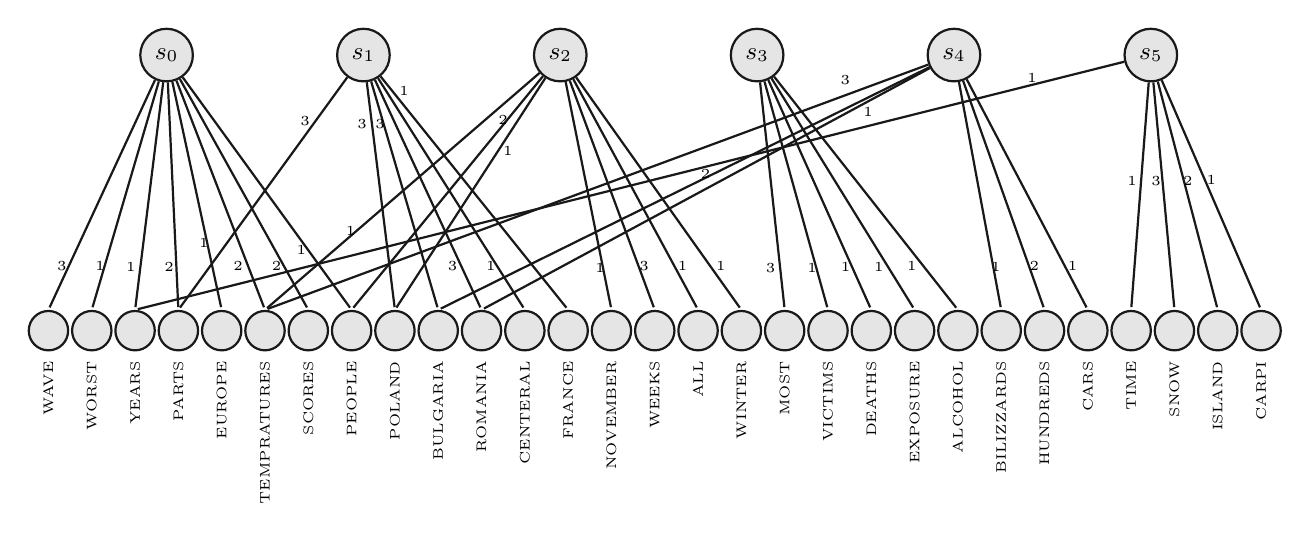
\begin{tikzpicture}[shorten >=1pt,-,scale=0.5]  
		\tikzstyle{sentence}=[circle,thick,draw=black!90,fill=black!10,minimum size=2mm]
	\tikzstyle{entity}=[circle,thick,draw=black!90,fill=black!10,minimum size=5mm]
		\tikzstyle{edge}=[draw=black!90, thick]
	   \begin{scope}
	   
		 \node [sentence] (s0) at (-3,0) {\small{$s_0$}};
		 \node [sentence] (s1) at (2,0) {\small{$s_1$}};
		 \node [sentence] (s2) at (7,0) {\small{$s_2$}}; 
		 \node [sentence] (s3) at (12,0) {\small{$s_3$}}; 
		 \node [sentence] (s4) at (17,0) {\small{$s_4$}};
		 \node [sentence] (s5) at (22,0) {\small{$s_5$}}; 
		 


	 \node [entity, label=below:\rotatebox{+90}{\tiny{WAVE}}] (e0)  at (-6.0,-7) {}; 
	 \node [entity, label=below:\rotatebox{+90}{\tiny{WORST}}] (e1)  at (-4.9,-7) {};
	 \node [entity, label=below:\rotatebox{+90}{\tiny{YEARS}}] (e2)  at (-3.8,-7) {}; 
	 \node [entity, label=below:\rotatebox{+90}{\tiny{PARTS}}] (e3)  at (-2.7,-7) {}; 
	 \node [entity, label=below:\rotatebox{+90}{\tiny{EUROPE}}] (e4)  at (-1.6,-7) {}; 
	 \node [entity, label=below:\rotatebox{+90}{\tiny{TEMPRATURES}}] (e5)  at (-0.5,-7) {}; 
	 \node [entity, label=below:\rotatebox{+90}{\tiny{SCORES}}] (e6)  at (0.6,-7) {}; 
	 \node [entity, label=below:\rotatebox{+90}{\tiny{PEOPLE}}] (e7)  at (1.7,-7) {}; 
	 \node [entity, label=below:\rotatebox{+90}{\tiny{POLAND}}] (e8)  at (2.8,-7) {}; 
	 \node [entity, label=below:\rotatebox{+90}{\tiny{BULGARIA}}] (e9)  at (3.9,-7) {}; 
	 \node [entity, label=below:\rotatebox{+90}{\tiny{ROMANIA}}] (e10)  at (5.0,-7) {}; 
	 \node [entity, label=below:\rotatebox{+90}{\tiny{CENTERAL}}] (e11)  at (6.1,-7) {}; 
	 \node [entity, label=below:\rotatebox{+90}{\tiny{FRANCE}}] (e12)  at (7.2,-7) {}; 
	 \node [entity, label=below:\rotatebox{+90}{\tiny{NOVEMBER}}] (e13)  at (8.3,-7) {}; 
	 \node [entity, label=below:\rotatebox{+90}{\tiny{WEEKS}}] (e14)  at (9.4,-7) {}; 
	 \node [entity, label=below:\rotatebox{+90}{\tiny{ALL}}] (e15)  at (10.5,-7) {}; 
	 \node [entity, label=below:\rotatebox{+90}{\tiny{WINTER}}] (e16)  at (11.6,-7) {}; 
	 \node [entity, label=below:\rotatebox{+90}{\tiny{MOST}}] (e17)  at (12.7,-7) {}; 
	 \node [entity, label=below:\rotatebox{+90}{\tiny{VICTIMS}}] (e18)  at (13.8,-7) {}; 
	 \node [entity, label=below:\rotatebox{+90}{\tiny{DEATHS}}] (e19)  at (14.9,-7) {}; 
	 \node [entity, label=below:\rotatebox{+90}{\tiny{EXPOSURE}}] (e20)  at (16.0,-7) {}; 
	 \node [entity, label=below:\rotatebox{+90}{\tiny{ALCOHOL}}] (e21)  at (17.1,-7) {}; 
	 \node [entity, label=below:\rotatebox{+90}{\tiny{BILIZZARDS}}] (e22)  at (18.2,-7) {}; 
	 \node [entity, label=below:\rotatebox{+90}{\tiny{HUNDREDS}}] (e23)  at (19.3,-7) {}; 
	 \node [entity, label=below:\rotatebox{+90}{\tiny{CARS}}] (e24)  at (20.4,-7) {}; 
	 \node [entity, label=below:\rotatebox{+90}{\tiny{TIME}}] (e25)  at (21.5,-7) {}; 
	 \node [entity, label=below:\rotatebox{+90}{\tiny{SNOW}}] (e26)  at (22.6,-7) {}; 
	 \node [entity, label=below:\rotatebox{+90}{\tiny{ISLAND}}] (e27)  at (23.7,-7) {}; 
	 \node [entity, label=below:\rotatebox{+90}{\tiny{CARPI}}] (e28)  at (24.8,-7) {}; 

		 
	 \path[edge] (s0) edge [above, very near end] node[font=\tiny] {$3$} (e0.north); %, line width=0.3ex
	 \path[edge] (s0) edge [above, very near end] node[font=\tiny] {$1$} (e1.north);
	 \path[edge] (s0) edge [above, very near end] node[font=\tiny, xshift=-1mm] {$1$} (e2.north);
	 \path[edge] (s0) edge [above, very near end] node[font=\tiny, xshift=-1mm] {$2$} (e3.north);
	 \path[edge] (s0) edge [above, very near end] node[font=\tiny, yshift=3mm, xshift=-1.5mm] {$1$} (e4.north);
	 \path[edge] (s0) edge [above, very near end] node[font=\tiny, xshift=-2mm] {$2$} (e5.north);
	 \path[edge] (s0) edge [above, very near end] node[font=\tiny, xshift=-2mm] {$2$} (e6.north);
	 \path[edge] (s0) edge [above, very near end] node[font=\tiny, yshift=2mm, xshift=-3.7mm] {$1$} (e7.north);

	 \path[edge] (s1) edge [above, near start] node[font=\tiny, near start] {$3$} (e3.north);
	 \path[edge] (s1) edge [above, near start] node[font=\tiny, xshift=-1.5mm] {$3$} (e8.north);
	 \path[edge] (s1) edge [above, near start] node[font=\tiny, xshift=-1mm] {$3$} (e9.north);
	 \path[edge] (s1) edge [above, very near end] node[font=\tiny, xshift=-2mm] {$3$} (e10.north);
	 \path[edge] (s1) edge [above, very near end] node[font=\tiny, xshift=-2mm] {$1$} (e11.north);
	 \path[edge] (s1) edge [above, very near start] node[font=\tiny] {$1$} (e12.north);

	 \path[edge] (s2) edge [above, very near end] node[font=\tiny, yshift=4.4mm, xshift=6.5mm] {$1$} (e5.north);
	 \path[edge] (s2) edge [above, near start] node[font=\tiny, xshift=1mm] {$2$} (e7.north);
	 \path[edge] (s2) edge [below, near start] node[font=\tiny] {$1$} (e8.north);
	 \path[edge] (s2) edge [below,  near end] node[font=\tiny] {$1$} (e13.north);
	 \path[edge] (s2) edge [above, very near end] node[font=\tiny] {$3$} (e14.north);
	 \path[edge] (s2) edge [above, very near end] node[font=\tiny] {$1$} (e15.north);
	 \path[edge] (s2) edge [above, very near end] node[font=\tiny] {$1$} (e16.north);

	 \path[edge] (s3) edge [below,  near end] node[font=\tiny,xshift=-1mm] {$3$} (e17.north);
	 \path[edge] (s3) edge [below,  near end] node[font=\tiny] {$1$} (e18.north);
	 \path[edge] (s3) edge [below,  near end] node[font=\tiny] {$1$} (e19.north);
	 \path[edge] (s3) edge [below,  near end] node[font=\tiny] {$1$} (e20.north);
	 \path[edge] (s3) edge [below,  near end] node[font=\tiny] {$1$} (e21.north);

	 \path[edge] (s4) edge [above, very near start] node[font=\tiny] {$3$} (e5.north);
	 \path[edge] (s4) edge [below, very near start] node[font=\tiny] {$1$} (e9.north);
	 \path[edge] (s4) edge [above, midway] node[font=\tiny] {$2$} (e10.north);
	 \path[edge] (s4) edge [above, very near end] node[font=\tiny] {$1$} (e22.north); 
	 \path[edge] (s4) edge [above, very near end] node[font=\tiny] {$2$} (e23.north); 
	 \path[edge] (s4) edge [above, very near end] node[font=\tiny] {$1$} (e24.north);     

	 \path[edge] (s5) edge [above, very near start] node[font=\tiny, xshift=4mm] {$1$} (e2.north);
	 \path[edge] (s5) edge [above, midway] node[font=\tiny,xshift=-1mm] {$1$} (e25.north);
	 \path[edge] (s5) edge [above, midway] node[font=\tiny,xshift=-1mm] {$3$} (e26.north);
	 \path[edge] (s5) edge [above, midway] node[font=\tiny] {$2$} (e27.north); 
	 \path[edge] (s5) edge [above, midway] node[font=\tiny] {$1$} (e28.north);    
		\end{scope}        
	  \end{tikzpicture}
\end{tabular}
\caption{The entity graph representation of the text in Table \ref{}.}
\label{f:entity_graph}
\end{figure}



Figure \ref{} shows how a bipartite graph captures the distribution of entities between sentences of a text. 


\subsection{Coherence Representation: Average Outdegree of Projection Graphs}
%
Coherence is almost about the connectivity of sentences of a text. 
Sentences are modeled as, just, one set of nodes in the entity graph representation.  
In graph theory, there are different ways to project a bipartite graph, which consists of two sets of nodes, into a graph whose nodes are only one set of nodes of the bipartite graph. 
This graph is called one-mode projection graph and its edges are obtained based on the other set of nodes of the bipartite graph. 
One-mode projection graphs can be weighted in different ways in order to retain the information of the bipartite graph. 


\newcite{guinaudeau13} apply one-mode projection \cite{newmanmark10} to the sentence nodes of the bipartite graph to represent the connections that exist between –- potentially non adjacent –- sentences in the graph. 
These projections result in graphs where nodes correspond to sentences and an edge is created between two nodes if the corresponding sentence node in the bipartite graph have at least one entity in common. 
Contrary to the bipartite graph, edges in one-mode projections are directed representing the order of sentences in texts. 



\newcite{guinaudeau13} apply three kinds of projections, $P_U$, $P_W$ and $P_{Acc}$, depending on
the weighting scheme associated with their edges. 
In, $P_U$, weights are binary and equal to $1$ where two sentences have a least one entity in common. 
This projection graph only shows the which sentences are linked to each other based on entity relations. 
In $P_W$, edges are weighted according to the number of entities ``shared” by two sentences. 
This projection graph is more informative than $P_U$ so that sentence nodes that are adjacent to more entity nodes in a bipartite graph are more strongly connected than those with less common entity nodes. 
In $P_{Acc}$ syntactic information is accounted for by integrating the edge weights in the bipartite graph. 
In this case, weights are equal to

\begin{equation}
W_{ik} = \sum_{e \in E_{ik}}{w(e,s_i) \cdot w(e,s_k)}
\end{equation}


where $E_{ik}$ is the set of entities shared by $s_i$ and $s_k$. 
This type of the projection graph is more informative than two others in this sense that it incorporate the grammatical information, which are roughly similar to syntactical transitions in the entity grid model, as weight of edges. 
Figure \ref{} shows $P_U$, $P_W$, and $P_{Acc}$ graphs obtained from the presented bipartite graph in Figure \ref{}.


\begin{figure}[!t]
\centering
\small

\begin{tabular}{lc}

\begin{tikzpicture}        
		 \node [] (n0) at (0,0) {};
         \node [] (label) at (0,0.8) {$P_U:$};
\end{tikzpicture}
&
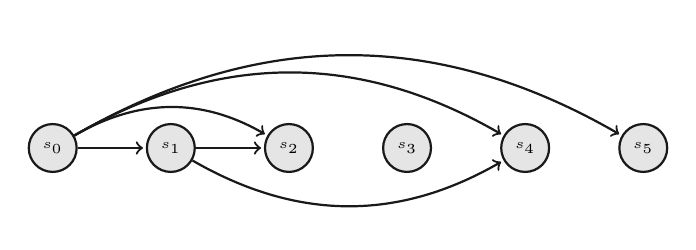
\begin{tikzpicture}[shorten >=1pt,->,scale=0.5]  
        \tikzstyle{sentence}=[circle,thick,draw=black!90,fill=black!10,minimum size=2mm]
		\tikzstyle{entity}=[circle,thick,draw=black!90,fill=black!10,minimum size=2mm]
        \tikzstyle{edge}=[draw=black!90, thick]

       \begin{scope}
       
         \node [sentence] (s0) at (0,0) {\tiny{$s_0$}};
         \node [sentence] (s1) at (3,0) {\tiny{$s_1$}};
         \node [sentence] (s2) at (6,0) {\tiny{$s_2$}}; 
         \node [sentence] (s3) at (9,0) {\tiny{$s_3$}}; 
         \node [sentence] (s4) at (12,0) {\tiny{$s_4$}};
         \node [sentence] (s5) at (15,0) {\tiny{$s_5$}}; 
 
 		\path[edge] (s0) edge [above] node[font=\tiny]{} (s1);
 		\path[edge, bend left = 30] (s0) edge [above] node[font=\tiny]{} (s2);
		\path[edge, bend left = 30] (s0) edge [above] node[font=\tiny]{} (s4);
 		\path[edge, bend left = 30] (s0) edge [above] node[font=\tiny]{} (s5);

 		\path[edge] (s1) edge [above] node[font=\tiny]{} (s2);
		\path[edge, bend right = 30] (s1) edge [above] node[font=\tiny]{} (s4);
           
        \end{scope}        
      \end{tikzpicture}

\\

\begin{tikzpicture}        
		 \node [] (n0) at (0,0) {};
         \node [] (label) at (0,0.8) {$P_W:$};
\end{tikzpicture}
 &
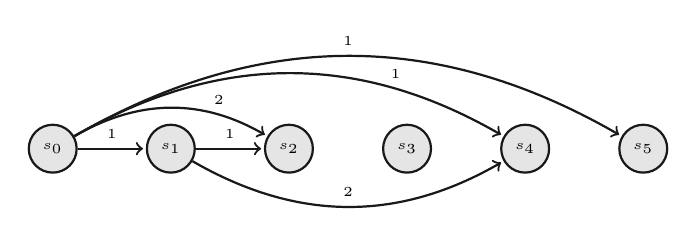
\begin{tikzpicture}[shorten >=1pt,->,scale=0.5]  
        \tikzstyle{sentence}=[circle,thick,draw=black!90,fill=black!10,minimum size=2mm]
		\tikzstyle{entity}=[circle,thick,draw=black!90,fill=black!10,minimum size=2mm]
        \tikzstyle{edge}=[draw=black!90, thick]

       \begin{scope}
       
         \node [sentence] (s0) at (0,0) {\tiny{$s_0$}};
         \node [sentence] (s1) at (3,0) {\tiny{$s_1$}};
         \node [sentence] (s2) at (6,0) {\tiny{$s_2$}}; 
         \node [sentence] (s3) at (9,0) {\tiny{$s_3$}}; 
         \node [sentence] (s4) at (12,0) {\tiny{$s_4$}};
         \node [sentence] (s5) at (15,0) {\tiny{$s_5$}}; 
 
 		\path[edge                ] (s0) edge [above, midway] node[font=\tiny]{$1$} (s1);
 		\path[edge, bend left = 30] (s0) edge [above, near end] node[font=\tiny]{$2$} (s2);
		\path[edge, bend left = 30] (s0) edge [above, near end] node[font=\tiny]{$1$} (s4);
 		\path[edge, bend left = 30] (s0) edge [above, midway] node[font=\tiny]{$1$} (s5);

 		\path[edge                 ] (s1) edge [above, midway] node[font=\tiny]{$1$} (s2);
		\path[edge, bend right = 30] (s1) edge [above, midway] node[font=\tiny]{$2$} (s4);
           
        \end{scope}        
      \end{tikzpicture}

\\

\begin{tikzpicture}        
		 \node [] (n0) at (0,0) {};
         \node [] (label) at (0,0.8) {$P_{Acc}:$};
\end{tikzpicture}
 &
   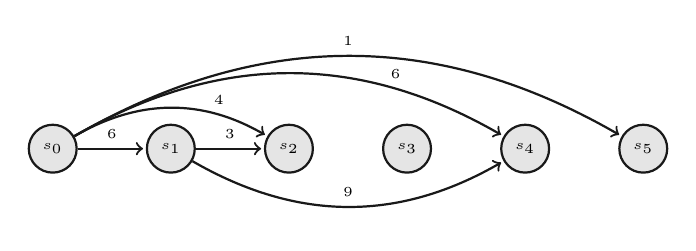
\begin{tikzpicture}[shorten >=1pt,->,scale=0.5]  
        \tikzstyle{sentence}=[circle,thick,draw=black!90,fill=black!10,minimum size=2mm]
		\tikzstyle{entity}=[circle,thick,draw=black!90,fill=black!10,minimum size=2mm]
        \tikzstyle{edge}=[draw=black!90, thick]

       \begin{scope}
       
         \node [sentence] (s0) at (0,0) {\tiny{$s_0$}};
         \node [sentence] (s1) at (3,0) {\tiny{$s_1$}};
         \node [sentence] (s2) at (6,0) {\tiny{$s_2$}}; 
         \node [sentence] (s3) at (9,0) {\tiny{$s_3$}}; 
         \node [sentence] (s4) at (12,0) {\tiny{$s_4$}};
         \node [sentence] (s5) at (15,0) {\tiny{$s_5$}}; 
 
 		\path[edge                ] (s0) edge [above, midway] node[font=\tiny]{$6$} (s1);
 		\path[edge, bend left = 30] (s0) edge [above, near end] node[font=\tiny]{$4$} (s2);
		\path[edge, bend left = 30] (s0) edge [above, near end] node[font=\tiny]{$6$} (s4);
 		\path[edge, bend left = 30] (s0) edge [above, midway] node[font=\tiny]{$1$} (s5);

 		\path[edge                 ] (s1) edge [above, midway] node[font=\tiny]{$3$} (s2);
		\path[edge, bend right = 30] (s1) edge [above, midway] node[font=\tiny]{$9$} (s4);
           
        \end{scope}        
      \end{tikzpicture}

\end{tabular}
\caption{$P_U$, $P_W$, and $P_{Acc}$ projection graphs.}

\label{f:entity_projection}
\end{figure}


Distance between sentences can be integrated in the weight of the one-mode projection graphs to decrease the importance of links that exist between nonadjacent sentences. 
In this case, the weights of the projection graphs are divided by the number of sentences in between of two sentences. 

Inspired from the centrality measure in graph theory that measures the connectivity of nodes in a graph, the coherence of a text can be measured by computing the average outdegree of a projection graph as follow:

\begin{equation}
Coh(T) = AvgOutDeg(P) = \frac{1}{N} \sum_{\textit{i \ in 1..N}} outDegree(s_i),
\end{equation}

where $outdegree(s_i)$ is the sum of the weights associated to edges that leave $s_i$ and $N$ is the number of nodes in graph $P$. 

In our running example the average outdegrees in different projection graphs are as follows:

\begin{table}[!ht]
\centering
\begin{tabular}{l|l}
\hline
 $P$ & $ AvgOutDeg(P) = Coh(T)$ \\\hline
 $P_U$ & $\frac{1}{6} \left((1+1+1+1)+(1+1)+(0)+(0)+(0)+(0)) \right) = 1.00$ \\
 $P_W$ & $\frac{1}{6} \left((1+2+1+1)+(1+2)+(0)+(0)+(0)+(0)) \right) = 1.33$\\
 $P_{Acc}$ &$\frac{1}{6} \left((6+4+6+1)+(3+9)+(0)+(0)+(0)+(0)) \right) = 4.83$ \\
 $P_U\textit{, }Dist$ & $\frac{1}{6} \left((1+0.50+0.25+0.20)+(1+0.33)+(0)+(0)+(0)+(0)) \right) = 0.55$ \\
 $P_W\textit{, }Dist$ & $\frac{1}{6} \left((1+1+0.25+0.20)+(1+0.66)+(0)+(0)+(0)+(0)) \right)= 0.69$ \\
 $P_{Acc}\textit{, }Dist$ & $\frac{1}{6} \left((6+2+1.5+0.2)+(3+3)+(0)+(0)+(0)+(0)) \right)= 2.61$ \\ \\
 \hline
\end{tabular}
\end{table}

It is worth to mention that the proposed entity graph model by \newcite{guinaudeau13} is an unsupervised model meaning that the final average outdegree can be directly used for comparing two texts with respect to their coherence. 
\newcite{guinaudeau13} assume that projection graphs of coherent texts contain more edges than the projection graph of  incoherent texts. 
Therefore, the projection graph of coherent texts are expected to have higher average outdegree than the projection graph of incoherent texts.  
That is the intuition of using average outdegree as a metric that measures the connectivity of nodes in projection graphs and consequently the coherence of texts. 


\section{The Normalized Entity Graph Model}
%
\subsection{Motivation}
%
The entity graph model uses the projection graph representation of a text to measure its coherence. 
As discussed above, depending on how weights of edges in projection graphs are computed, different types of projection graphs can be proposed. 
Based on what information of the entity graph is critical to be transfered to projection graphs weights of the projection graphs are computed.
For example, $P_U$, which is the basic projection graph proposed by \newcite{guinaudeau13}, only captures this information of  entity graphs that if two sentence nodes have an entity node in common. 
$P_W$ is more informative and sets the number of common entities between two sentence nodes in the entity graph as a weight to the edge that connects those sentences nodes in the projection graph. 
$P_{Acc}$ incorporates grammatical transitions of common entities between sentence nodes of the entity graph in the process of weight calculation of edges of projection graphs. 


An important information that is used in the entity grid model but is missed in the entity graph model is the salience of entities. 
In the entity grid model the frequency of an entity\footnote{Frequency of an entity means the number of mentions of an entity in a text.} is considered an indicator of its importance. 
However, the importance of an entity in a sentence depends on many factors such as its syntactical role, the number of mentioned entities in that sentence, and etc. 
With this motivation we propose a new version of the entity graph model that takes into account the importance of entities and sentences based on the topology of the entity graph. 

The normalization is applied on weights of the entity graph and then one-mode projections. 
The normalization is based on the relative importance of entities and, in turn, the relative importance of sentences. 
Including negative information, such as the number of a sentence's entities that are not shared with other sentences, allows to normalize the importance of entities according to sentence length (measured in terms
of entity mentions), and hence to capture distance information between mentions of the same entity.
This brings the entity graph closer to \newcite{stoddard91,p.30} notion of cohesion: ``The relative cohesiveness of a text depends on the number of cohesive ties [...] and on the distance between the nodes and their associated cohesive elements.” By using this information, edge weights are set less arbitrary. 
Normalization also allows to include distance between mentions of the same entity.  

As it stated in \cite{zhoudengyong07,zweig11} that normalizing weights leads to better performance. 

\subsection{Text Representation: Normalized Entity Graph}
%
We employ the entity graph representation for modeling the distribution of entities over adjacent sentences. 
As a recall, this graph is weighted and the weight of each edge represents the grammatical role of each entity in each sentence.  


The definition of silence has two sides. 
One side is that salient entities are mentioned in important sentences.  
On the other side, important sentences contain salient entities and they are connected to each other because they share salient entities. 
That is why we approach to salience as a relative concept where the salience of an entity is computed with respect to other entities and sentences in a text. 

Our intuition is inspired by information retrieval where each sentence is supposed to carry a piece of information in a text. 
In entity-based coherence models, entities make information that is included in a sentence. 
When a sentence contains many entities it gets more difficult for a reader to process the expressed relation between entities in the sentence. 
This is roughly captured by readability formulas in that texts with long sentences are more difficult to read because they take more processing time of their readers. 
On the other hand, sentences that contain most entities that are mentioned in a text are more important than other sentences, because they contain most information of a text. 

Our normalization process defines a trade off between the above factors in a text.  
The normalization process consists of two main steps: how important is an entity for each individual sentence, and how important is a sentence for a text. 


Here we normalize the weights of mentioned entities in a sentence with respect to the weight of the rest of entities in the sentence. 
This takes negative information into account as entities which do not occur in other sentences also count. 
We follow \newcite{newmanmark10} by applying node degree normalization. 

Given an entity graph, the normalized weight of an edge that connect an entity node, $e$, to a sentence node, $s$, equals the current weight of that edge divided by the sum of weights of edges that are connected to the sentence node, $s$. 
This gives the importance of each entity in a sentence relative to the sentence’s other entities.

\begin{equation}
Imp(s,e) = \frac{w(s,e)}{\sum_{e^{`}\in Entities}{w(s,e^{`})}}.
\end{equation} 

Moreover, in order to compute the relative importance of sentences with respect to each other, we measure what portion of information in a text is present in each sentence. 
Since we are modeling local coherence, for any pair of sentences we compute their relative importance. 
Following \cite{rode08}, we use the following formula to compute the relative importance of each sentence:

\begin{equation}
w(s_i, s_j) = \frac{||s_i||}{||s_i|| + ||s_j ||},
\end{equation}

This value is equal to the degree of each sentence in the entity graph.  

\subsection{Coherence Representation: Normalized Projection Graph}
%
Similar to the entity graph model, we use the one-mode projection graph of the entity graph representation to encode the connections between sentences. 
Then we compute the average outdegree of nodes in projection graphs as a measure of coherence. 

Since $P_U$ is not weighted the normalization does not affect this projection graph. 

Above we explained how we normalize an entity graph. 
Since the grammatical roles of entities are not used in $P_w$,  we assume that the entity graph is unweighted. 
So the normalization process is just dividing the weight of each edge in the entity graph by the degree of the corresponding sentence node. 
If a sentence contains many entities, then the amount of information each entity contributes is reduced.
Assume $||s||$ as the number of entities in sentence $s$.  
The importance of entity $e$ for $s$ is 

\begin{equation}
Imp(s,e) = \frac{1}{||s||}.
\end{equation}

For $P_{Acc}$, we follow the normalization process as it is explained above. 
The entity graph model weighs edges by the number of entities sentences share ($P_W$) and which syntactic functions the entities occupy ($P_{Acc}$). 


Regardless of what type of projection graph we are building, the weight of the edge that connects sentences $s_i$ and $s_j$ is:

\begin{equation}
W(s_i,s_j) = \sum_{e \in E_i+E_j}{(w_{s_i}^{s_j}.Imp(s_i,e))+(w_{s_j}^{s_i}.Imp(s_j,e))}.
\end{equation}

Intuitively, the above equation computes the local coherence between any pair of sentences. 
Given a pair of sentences, the sentence that contains more entities is more informative and almost more important while the importance of entities in longer sentences are more discarded. 
Similar to \cite{rode08}, we use the product of $w_{s_i}^{s_j}$ and $Imp(s_i; e)$ to approximate the local salience of entity $e$ in each sentence $s_i$. 
This prevents the model to get biased by the length of sentences. 

Figure \ref{fig:normalized_entity_projection} depicts normalized version of the projection graphs presented in Figure \ref{}. 

\begin{figure}[!t]
\centering
\small

\begin{tabular}{lc}

\begin{tikzpicture}        
		 \node [] (n0) at (0,0) {};
         \node [] (label) at (0,0.8) {$P_U:$};
\end{tikzpicture}
&
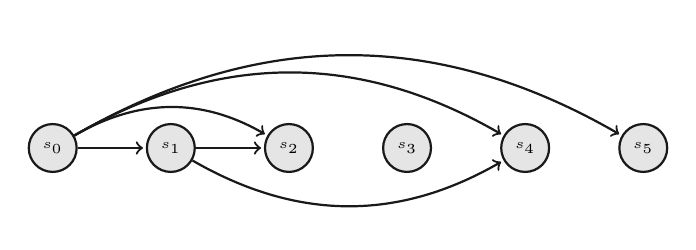
\begin{tikzpicture}[shorten >=1pt,->,scale=0.5]  
        \tikzstyle{sentence}=[circle,thick,draw=black!90,fill=black!10,minimum size=2mm]
		\tikzstyle{entity}=[circle,thick,draw=black!90,fill=black!10,minimum size=2mm]
        \tikzstyle{edge}=[draw=black!90, thick]

       \begin{scope}
       
         \node [sentence] (s0) at (0,0) {\tiny{$s_0$}};
         \node [sentence] (s1) at (3,0) {\tiny{$s_1$}};
         \node [sentence] (s2) at (6,0) {\tiny{$s_2$}}; 
         \node [sentence] (s3) at (9,0) {\tiny{$s_3$}}; 
         \node [sentence] (s4) at (12,0) {\tiny{$s_4$}};
         \node [sentence] (s5) at (15,0) {\tiny{$s_5$}}; 
 
 		\path[edge] (s0) edge [above] node[font=\tiny]{} (s1);
 		\path[edge, bend left = 30] (s0) edge [above] node[font=\tiny]{} (s2);
		\path[edge, bend left = 30] (s0) edge [above] node[font=\tiny]{} (s4);
 		\path[edge, bend left = 30] (s0) edge [above] node[font=\tiny]{} (s5);

 		\path[edge] (s1) edge [above] node[font=\tiny]{} (s2);
		\path[edge, bend right = 30] (s1) edge [above] node[font=\tiny]{} (s4);
           
        \end{scope}        
      \end{tikzpicture}

\\

\begin{tikzpicture}        
		 \node [] (n0) at (0,0) {};
         \node [] (label) at (0,0.8) {$P_W:$};
\end{tikzpicture}
 &
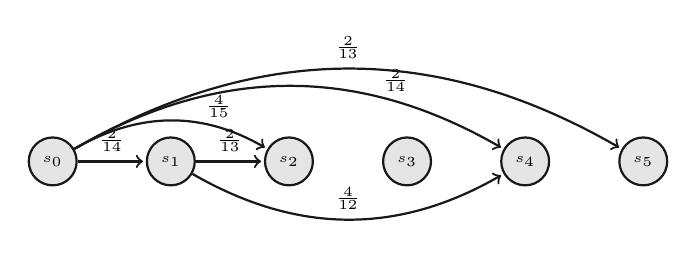
\begin{tikzpicture}[shorten >=1pt,->,scale=0.5]  
        \tikzstyle{sentence}=[circle,thick,draw=black!90,fill=black!10,minimum size=2mm]
		\tikzstyle{entity}=[circle,thick,draw=black!90,fill=black!10,minimum size=2mm]
        \tikzstyle{edge}=[draw=black!90, thick]

       \begin{scope}
       
         \node [sentence] (s0) at (0,0) {\tiny{$s_0$}};
         \node [sentence] (s1) at (3,0) {\tiny{$s_1$}};
         \node [sentence] (s2) at (6,0) {\tiny{$s_2$}}; 
         \node [sentence] (s3) at (9,0) {\tiny{$s_3$}}; 
         \node [sentence] (s4) at (12,0) {\tiny{$s_4$}};
         \node [sentence] (s5) at (15,0) {\tiny{$s_5$}}; 
 
 		\path[edge                ] (s0) edge [above, midway] node[font=\tiny]{$\frac{2}{14}$} (s1);
 		\path[edge, bend left = 30] (s0) edge [above, near end] node[font=\tiny]{$\frac{4}{15}$} (s2);
		\path[edge, bend left = 30] (s0) edge [above, near end] node[font=\tiny]{$\frac{2}{14}$} (s4);
 		\path[edge, bend left = 30] (s0) edge [above, midway] node[font=\tiny]{$\frac{2}{13}$} (s5);

 		\path[edge                 ] (s1) edge [above, midway] node[font=\tiny]{$\frac{2}{13}$} (s2);
		\path[edge, bend right = 30] (s1) edge [above, midway] node[font=\tiny]{$\frac{4}{12}$} (s4);
           
        \end{scope}        
      \end{tikzpicture}

\\

\begin{tikzpicture}        
		 \node [] (n0) at (0,0) {};
         \node [] (label) at (0,0.8) {$P_{Acc}:$};
\end{tikzpicture}
 &
   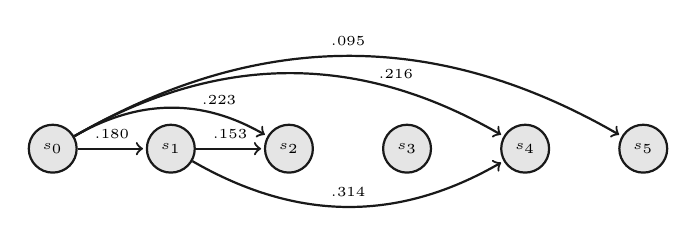
\begin{tikzpicture}[shorten >=1pt,->,scale=0.5]  
        \tikzstyle{sentence}=[circle,thick,draw=black!90,fill=black!10,minimum size=2mm]
		\tikzstyle{entity}=[circle,thick,draw=black!90,fill=black!10,minimum size=2mm]
        \tikzstyle{edge}=[draw=black!90, thick]

       \begin{scope}
       
         \node [sentence] (s0) at (0,0) {\tiny{$s_0$}};
         \node [sentence] (s1) at (3,0) {\tiny{$s_1$}};
         \node [sentence] (s2) at (6,0) {\tiny{$s_2$}}; 
         \node [sentence] (s3) at (9,0) {\tiny{$s_3$}}; 
         \node [sentence] (s4) at (12,0) {\tiny{$s_4$}};
         \node [sentence] (s5) at (15,0) {\tiny{$s_5$}}; 
 
 		\path[edge                ] (s0) edge [above, midway] node[font=\tiny]{$.180$} (s1);
 		\path[edge, bend left = 30] (s0) edge [above, near end] node[font=\tiny]{$.223$} (s2);
		\path[edge, bend left = 30] (s0) edge [above, near end] node[font=\tiny]{$.216$} (s4);
 		\path[edge, bend left = 30] (s0) edge [above, midway] node[font=\tiny]{$.095$} (s5);

 		\path[edge                 ] (s1) edge [above, midway] node[font=\tiny]{$.153$} (s2);
		\path[edge, bend right = 30] (s1) edge [above, midway] node[font=\tiny]{$.314$} (s4);
           
        \end{scope}        
      \end{tikzpicture}

\end{tabular}
\caption{$P_U$, $P_W$, and $P_{Acc}$ normalized projection graphs.}
\label{fig:normalized_entity_projection}
\end{figure}


Table \ref{} shows the outdegree of each projection graph. 


\section{Experiments}
%
In this section, we compare the introduced local coherence models (i.e., the entity graph model, the entity grid model, and the normalized entity graph model) in three benchmark tasks: sentence ordering, summary coherence ranking, and readability assessment. 
We show that although the entity graph model is an unsupervised model, it outperforms the entity grid model (as a supervised model) on these tasks. 
This shows that graphs are a suitable framework to model coherence of a text. 
We evaluate our proposed normalization on the entity graph model and show that our normalized entity graph model obtains a higher performance than the entity graph model. 
This indicates that the entity graph model is a good framework but it is far away from perfect and can be improved.  
The results of our experiments in this chapter motive us to consider the entity graph representation of texts for developing new coherence features and model. 


% We compare the normalized entity graph with the entity graph on all tasks, Guinaudeau and Strube
% (2013) compared their work with the entity grid (Barzilay and Lapata, 2008; Elsner and Charniak,
% 2011): sentence ordering, summary coherence rating and readability assessment. 
% Following Guinaudeau and Strube (2013) we test statistical significance with the Student’s t-test and Bonferroni
% correction, to check whether the best result (bold value in the tables) is significantly different from
% the results of the entity graph and the normalized entity graph. 
% Diacritics ** indicate significance level 0.01, * indicates significance level 0.05.

\subsection{Sentence Ordering}
%
It is known that the order of information in coherent texts is such that they are easy to follow \cite{lapata03,barzilay04,karamanis04b,barzilay05a,soricut06}. 
As it is explained in the definition of coherence, a text is more than a random concatenation of sentences;
the order of sentences affects how difficult the presented information in a text can be understood, if at all. 
Given the above fact, a document can be taken as an unordered bag of sentences and the task would be to find the ordering of the sentences that maximizes coherence according to a model. 
Unfortunately, finding the best ordering is NP-complete \cite{?} and non-approximable \cite{althaus04}.
Therefore, this task need to be simplified to be used for coherence evaluation. 
Two restricted versions of the sentence ordering tasks are the discrimination task, and the insertion task. 
In both subtasks we evaluate whether our model is able to distinguish between the correct (original) order of sentences in a document and an incorrect (non-original) one. 

\subsubsection{Discrimination}
%
The discrimination task is based on this fact that the original order of sentences in a document is taken as the best order and any scrambling of sentences disturbs the perceived coherence of the document. 
Therefore, by rearranging the order of sentences of a document, we are making the document more difficult to understand or less coherent, because the order of presented information is disturbed. 

More formally, let $COH_M(d)$ be the coherence estimation of document $d$ by the coherence model $M$ and $p$ be a version of $d$ that its sentences are randomly permuted, then the coherence model $M$ should ideally distinguish document $d$ a more coherent document than $p$:

\begin{equation}
COH_M(d) > COH_M(p). 
\end{equation}


\paragraph{Setting}
%
We use the same setting that is used in \newcite{guinaudeau13}. 
$61$ documents are extracted from the English test part of the CoNLL $2012$ shared task \cite{pradhan12}. 
Documents are composed of $36.1$ sentences and $2064$ word tokens on average. 

In this experiment, a model associates local coherence values with the original document and its permutation, if the score for the original order of sentences of a document is higher than the score of the permutation version of sentence then the output of our system being considered correct. 

We use $20$ permutations of each text. 
Because we do not know the relative quality of different permutations, the dataset includes only pairwise rankings that comprise the original document and one of its permutations.

We employ two evaluation metrics: accuracy and F-measure. 
Accuracy is used to evaluate how correctly a coherence model discriminates the original order of a document from its $20$ different permutations.
It equals the number of times the model gives a higher score to the original document than the score that it gives to a permutation, divided by the number of comparisons.

\begin{equation}
Acc  = \frac{\#\textit{ of correct predictions}}{\#\textit{ of comparisons}}
\end{equation}

We also computed F-measure because the model may give the same score to a permutation and the original document. 
In order to compute F-measure, we need to compute recall and precision as follow:

\begin{equation}
recall = \frac{correct}{total},
\end{equation}
where $total$ is the total number of test samples no matter if on them the model can make a decision or not. 

\begin{equation}
precision = \frac{correct}{decisions},
\end{equation}
where $decision$ is the number of samples on that the model made a decision.

\begin{equation}
F1 = 2.\frac{precision \cdot recal}{precision + recall}
\end{equation}


We test significance by the Student’s t-test that detects statistically significant differences between paired samples.
Moreover, as increasing the number of hypotheses in a test can also increase the likelihood of witnessing a rare event, and therefore, the chance to reject the null hypothesis when it is true, we use the Bonferroni correction to adjust the increased
random likelihood of apparent significance. 

In contrast the entity graph model, the entity grid model is a supervised model. 
The above setting makes it easy to define a machine learning setup for the entity grid model. 
Following \newcite{barzilay08}, if we assume that the $COH_M(d)$ is a linear function of coherence features, which are defined as the entity transitions in the entity grid model as follows:

\begin{equation}
COH_M(d) = \vec{w}^{T}.\vec{t}
\end{equation}

where $w$ is a vector of parameters and $t$ is the feature vector representing the coherence of $d$. 
The goal of the learning procedure is learn the best values for parameters $w$ in order to minimize the number of violations of pairwise rankings provided in the training set:

\begin{equation}
COH_M(d) > COH_M(p)
\end{equation}

The problem typically treated as a Support Vector Machine (SVM) constraint optimization problem, and can be solved using the search technique implemented in $SVM_{ligh}$\footnote{link to the package} \cite{joachims02} package. 

Similar to \newcite{guinaudeau13} we do not use the ACCIDENTS and EARTHQUAKES datasets that are employed in the entity grid model. 
\newcite{guinaudeau13}'s main reason is that, as  it is also mentioned by \newcite{elsner08b}, the ACCIDENTS and EARTHQUAKES datasets use a very constrained style and are not typical of normal informative documents. 


For entity extractions all nouns in a document are considered discourse entities, even those that do not head NPs.
Nouns and grammatical information associated with each entity is extracted automatically thanks to the Stanford parser \cite{marneffe06} and Brown Coherence Toolkit \footnote{\url{https://bitbucket.org/melsner/}}. 



Results for \newcite{guinaudeau13}, G\&S, are reproduced, results for 
B\&L \newcite{barzilay08}, and E\&C \newcite{elsner11b},  are reported from \newcite{guinaudeau13}. 


\begin{table}[!t]
\centering
\begin{small}
\begin{tabular}{l|cc@{}l}
& Acc & F &\\\hline
Random & 0.496 & 0.496 & \\
B\&L & 0.877 & 0.877 &\\ 
E\&C & 0.915 & 0.915  &\\\hline

& \multicolumn{3}{|c}{Entity graph, G\&S} \\\hline 
$P_U$, \textit{Dist} & 0.830 & 0.830 & ** \\
$P_W$, \textit{Dist} & 0.871 & 0.871& \\
$P_{Acc}$, \textit{Dist} & 0.889 & 0.889& \\\hline

& \multicolumn{3}{|c}{Normalized entity graph} \\\hline 
$P_U$, \textit{Dist} & 0.830 & 0.830& ** \\
$P_W$, \textit{Dist} & 0.886 & 0.886&\\
$P_{Acc}$, \textit{Dist} & \textbf{0.909} & \textbf{0.909}&\\
\end{tabular}
\end{small}
\caption{Discrimination: baselines and entity graph vs.\ normalized
  entity graph}\label{t:exp1:sentence_ordering}  
\end{table}
%
In this experiment, the distance factor is crucial for the entity graph model and its normalized version. 
unlike the entity grid model, these two models do not incorporate the order of grammatical transitions. 
For instance, both transitions $S O$ and $O S$ yield the same edge weight, $6$, in the weighted projection graph, $P_{Acc}$. 
Moreover, an original document and its permutations contain the same entities. 
So without the distance factor these two models cannot distinguish between a document and its permutation. 
Intuitively, distance can model if sentences that share entities are located near to each other in a document or not. 
This is expected from coherent texts that neighboring sentences be about similar topics and therefore information of these sentences would be similar. 

The unweighted graph, $P_U$ is not weighted and it does not need any normalization.  
Hence the results for the entity graph and the normalized entity graph are identical.
Both are better than the Random baseline and worse than the performance of the B\&L model.
However, this projection graph is less informative than the B\&L model. 
Normalization improves the results for the weighted graphs $P_W$ and $P_{Acc}$ with $P_{Acc}$ outperforming B\&L
considerably and closely approaching E\&L. 
The results of this experiment show that our normalization model can transfer more information about the entity graph representation of a text to its projection graphs and improves the performance of the original entity graph model. 

The $P_{Acc}, Dist$ setting does not outperform E\&C model. 
It is important to note that the E\&C model is a supervised model and during training the model tunes the associated weights with entity transitions in order to obtain a better performance. 
In contrast, the entity graph model is an unsupervised model and its procedure is the same for any domain and task. 
Obtaining a competitive result near to a supervised model is promising.  


As we can see the performance of examined coherence models on the discrimination task are already high. 
It is mainly because the discrimination task can be easily solved without any notions of coherence. 
Discrimination specially becomes easier for longer documents, since the average random permutation grows less similar to the original document. 
The insertion task, the second related task to sentence ordering, somewhat overcomes this easiness. 


\subsubsection{Insertion}
%
Similar to the discrimination task, the insertion task \cite{chenerdong07} is designed to evaluate the ability of a coherence model in distinguishing the proper order of sentences in a document from the other orders. 
As we discussed, especially for documents with many sentences, permuting whole sentences yields a version of document that is very different, and therefore easier to distinguish, from the original document. 

The intuition behind the insertion task is that given a document where one of its sentences is removed, the perceived coherence 
of the document is discarded. 
A coherence model should be able to assign a higher coherence score to a permutation in that the removed sentence is located in its original position. 

Given a document with $n$ sentences, if the sentence at position $i$ is removed then there are $n$ possible positions, including the position $i$, to reinsert this sentence and create a permutation of this document. 
Table \ref{table:insertion_task} shows an example of removing the sentence in position $0$ ($\underline{A}$) of a document with four sentences, $\left \{ A, B, C, D \right \}$, and reinserting the sentence in all possible positions. 
 

\begin{table}[!ht]
\centering
\begin{small}
\begin{tabular}{cc|cccc}
position & original document  & \multicolumn{4}{c}{permutations}\\
\hline
$0$ & $\underline{A}$ & $\underline{A}$ & $B$ & $B$ & $B$\\
$1$ & $B$ 			  & $B$  & $\underline{A}$ & $C$ & $C$\\
$2$ & $C$			  & $C$ & $C$ & $\underline{A}$ & $D$\\
$3$ & $D$			  & $D$ & $D$ & $D$ & $\underline{A}$\\
\end{tabular}
\end{small}
\caption{}
\label{table:insertion_task}  
\end{table}

Besides any practical applications, insertion has two properties that make it well-suited for evaluation of coherence models. 
First, a document with $n$ sentences can be evaluated exactly in $n^2$ time, which, though it can be significant, is
still much faster than ordering and does not involve a potentially error-prone search.
Second, it grows more difficult as documents lengthen because permutations only differ by one sentence, unlike discrimination, which grow easier. 
Third, a document is compared to many more permutations in insertion task than in discrimination. 


For evaluation, we employ two evaluation metrics: accuracy and the insertion score (Ins.). 
Accuracy measures for how many sentences, out of the all sentences of a document, a coherence model exactly predicts the original position of the sentence as the best point to reinsert it. 
%(We report the average proportion of correct insertions per document.)
Therefore the accuracy is computed as follows:

\begin{equation}
Acc = \frac{1}{D}\sum_{d \in D}\frac{\#\textit{ of correctly placed sentences in d}}{\#\textit{ of sentences in d}}
\end{equation}
%
where $D$ is the set of documents in a dataset.  
By averaging over over documents, longer documents do not disproportionally influence the results. 

In complement to accuracy, we use the insertion score introduced by 
\newcite{elsner11b} for evaluation. 
This score  –- the higher, the better –-  is a positional score that measures how far the predicted position of a sentence by a coherence model is from the original position of the sentence. 
For each document this score is normalized by the length of document to be unbiased to the number of sentences in a document. 

More formally, this score is computed as follows:
\begin{equation}
Ins. = 1 - \frac{o - p}{norm(N, p)},
\end{equation}


\begin{equation}
norm(N, p) = \frac{1}{2*N} (p * (p-1) + (N - p + 1)*(N - p)),
\end{equation}
%
where $o$ and $p$ are respectively the original position of a removed sentence and its proposed position by the model. 
$N$ is the number of sentences in a document.  

We follow the same dataset that is used in the discrimination task.  
The system output is considered correct if the document associated with the highest local coherence score is
the one in which the sentence is reinserted in the correct position. 

We define a heuristic baseline to compare our models with. 
Since for a document with $n$ sentences, each sentence insertion is an n-way decision, a random baseline is expected that decision are sampled from an uniform distribution. 
For example for a document with two sentences, the probability of randomly predicting correctly is $50\%$. 
Thus, the random performance scales as $\frac{1}{n}$, going to zero as length increases.

\begin{table}[!b]
\centering
\begin{small}
\begin{tabular}{l|c@{}lc@{}l} 

		& Acc. & 	& Ins.  & \\\hline
 Random & $0.028$ & 	& $0.071$ & \\
 E\&C	& $0.068$ & 	& $0.167$ & \\\hline

		& \multicolumn{4}{|c}{Entity graph, G\&S} \\\hline 
 $P_U$, \textit{Dist} & $0.062$&** & $0.101$ & **\\
 $P_W$, \textit{Dist} & $0.075$& 	   & $0.114$ & **\\
 $P_{Acc}$, \textit{Dist} & $0.071$& 	 & $0.102$ & ** \\\hline
  & \multicolumn{4}{|c}{Normalized entity graph} \\\hline 
 $P_U$, \textit{Dist} & $0.062$&** & $0.101$ & **  \\
 $P_W$, \textit{Dist} & $\textbf{0.085}$& 	 & $\textbf{0.154}$&\\
 $P_{Acc}$, \textit{Dist} & $0.077$& 	 & $0.157$ & \\
\end{tabular}
\end{small}
\caption{Insertion, baselines and entity graph vs.\ normalized entity
  graph}\label{table:insertion_results} 
\end{table}

As expected, accuracies for this task are much lower than those obtained for discrimination, confirming this intuition that the insertion task is more difficult than the discrimination task. 
Similar to the discrimination task and with the same reasons, distance information is critical for the insertion task as well. 
So we compare the setting of the model that distance information is involved. 
In terms of accuracy, the $P_w$ projection information outperforms the baseline models (i.e., Random and E\&C). 
This indicates that the entity graph representation is a suitable framework for coherence modeling. 
Table  \ref{table:insertion_results} also shows that the normalized versions of the entity graph outperforms their counterparts projections in the entity graph model and normalized $P_w$ obtains the best accuracy. 
We see that for both entity graph and normalized entity graph models, using the syntactical information of entities do not improve the accuracy of these models. 
A reason for this is that by combining the weights of syntactical roles of the common entities between two sentences of an entity graph into the weight of the connecting edge between the sentences in $P_{Acc}$ the impact of the distance information is vanished.  
The presented example in Figure \ref{fig:pacc_vanishing_problem} illustrates this. 

\begin{figure}[!t]
\centering
\small
\begin{tabular}{@{}clclc@{}}
\hline
Projection & Sentence order &  Graph & Outdegree & Decision 
\\\hline
\multirow{2}{*}{$P_W$ }
&

\begin{tikzpicture}        
		 \node [] (n0) at (0,0) {};
         \node [] (label) at (0,0.8) {$original$};
\end{tikzpicture}
&
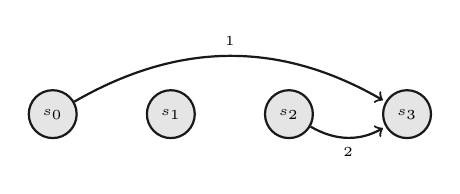
\begin{tikzpicture}[shorten >=1pt,->,scale=0.5]  
        \tikzstyle{sentence}=[circle,thick,draw=black!90,fill=black!10,minimum size=2mm]
		\tikzstyle{entity}=[circle,thick,draw=black!90,fill=black!10,minimum size=2mm]
        \tikzstyle{edge}=[draw=black!90, thick]

       \begin{scope}
       
         \node [sentence] (s0) at (0,0) {\tiny{$s_0$}};
         \node [sentence] (s1) at (3,0) {\tiny{$s_1$}};
         \node [sentence] (s2) at (6,0) {\tiny{$s_2$}}; 
         \node [sentence] (s3) at (9,0) {\tiny{$s_3$}}; 
 
 		\path[edge, bend left = 30] (s0) edge [above] node[font=\tiny]{$1$} (s3);
 		\path[edge, bend right = 30] (s2) edge [below] node[font=\tiny]{$2$} (s3);
           
        \end{scope}        
      \end{tikzpicture}

 &
 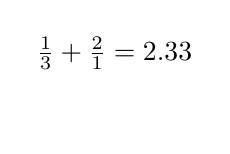
\begin{tikzpicture}        
		 \node [] (n0) at (0,0) {};
         \node [] (label) at (0,0.8) { $ \frac{1}{3} + \frac{2}{1}  = 2.33 $};
\end{tikzpicture}
&

\multirow{2}{*}{
\begin{tabular}{c}
$ 2.33 > 2 \Rightarrow $
\\
$correct$  
\end{tabular}
}
\\

&
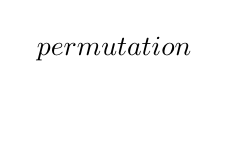
\begin{tikzpicture}        
		 \node [] (n0) at (0,0) {};
         \node [] (label) at (0,0.8) {$permutation$};
\end{tikzpicture}
&
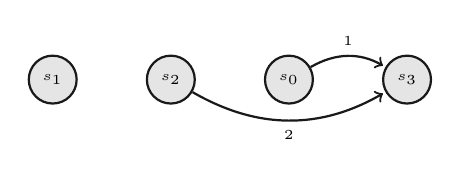
\begin{tikzpicture}[shorten >=1pt,->,scale=0.5]  
        \tikzstyle{sentence}=[circle,thick,draw=black!90,fill=black!10,minimum size=2mm]
		\tikzstyle{entity}=[circle,thick,draw=black!90,fill=black!10,minimum size=2mm]
        \tikzstyle{edge}=[draw=black!90, thick]

       \begin{scope}
       
         \node [sentence] (s1) at (0,0) {\tiny{$s_1$}};
         \node [sentence] (s2) at (3,0) {\tiny{$s_2$}};
         \node [sentence] (s0) at (6,0) {\tiny{$s_0$}}; 
         \node [sentence] (s3) at (9,0) {\tiny{$s_3$}}; 
 
 		\path[edge, bend left = 30] (s0) edge [above] node[font=\tiny]{$1$} (s3);
 		\path[edge, bend right = 30] (s2) edge [below] node[font=\tiny]{$2$} (s3);
           
        \end{scope}        
      \end{tikzpicture}

 &
 \begin{tikzpicture}        
		 \node [] (n0) at (0,0) {};
         \node [] (label) at (0,0.8) { $\frac{1}{1} + \frac{2}{2} =  2 $};
\end{tikzpicture}
&

\\ 
\hline
\\ 
\multirow{2}{*}{$P_{Acc}$ }
&


\begin{tikzpicture}        
		 \node [] (n0) at (0,0) {};
         \node [] (label) at (0,0.8) {$original$};
\end{tikzpicture}
&
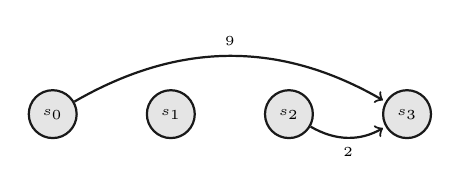
\begin{tikzpicture}[shorten >=1pt,->,scale=0.5]  
        \tikzstyle{sentence}=[circle,thick,draw=black!90,fill=black!10,minimum size=2mm]
		\tikzstyle{entity}=[circle,thick,draw=black!90,fill=black!10,minimum size=2mm]
        \tikzstyle{edge}=[draw=black!90, thick]

       \begin{scope}
       
         \node [sentence] (s0) at (0,0) {\tiny{$s_0$}};
         \node [sentence] (s1) at (3,0) {\tiny{$s_1$}};
         \node [sentence] (s2) at (6,0) {\tiny{$s_2$}}; 
         \node [sentence] (s3) at (9,0) {\tiny{$s_3$}}; 
 
 		\path[edge, bend left = 30] (s0) edge [above] node[font=\tiny]{$9$} (s3);
 		\path[edge, bend right = 30] (s2) edge [below] node[font=\tiny]{$2$} (s3);
           
        \end{scope}        
      \end{tikzpicture}

 &
 \begin{tikzpicture}        
		 \node [] (n0) at (0,0) {};
         \node [] (label) at (0,0.8) { $\frac{9}{3} + \frac{2}{1} = 5 $};
\end{tikzpicture}
&

\multirow{2}{*}{
\begin{tabular}{c}
$ 5 < 10 \Rightarrow $
\\
 $incorrect$
 \end{tabular}  
}
\\

&
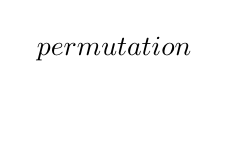
\begin{tikzpicture}        
		 \node [] (n0) at (0,0) {};
         \node [] (label) at (0,0.8) {$permutation$};
\end{tikzpicture}
&
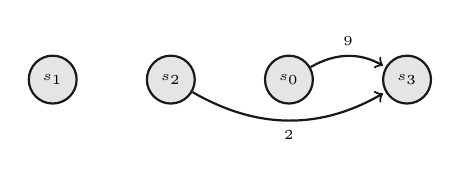
\begin{tikzpicture}[shorten >=1pt,->,scale=0.5]  
        \tikzstyle{sentence}=[circle,thick,draw=black!90,fill=black!10,minimum size=2mm]
		\tikzstyle{entity}=[circle,thick,draw=black!90,fill=black!10,minimum size=2mm]
        \tikzstyle{edge}=[draw=black!90, thick]

       \begin{scope}
       
         \node [sentence] (s1) at (0,0) {\tiny{$s_1$}};
         \node [sentence] (s2) at (3,0) {\tiny{$s_2$}};
         \node [sentence] (s0) at (6,0) {\tiny{$s_0$}}; 
         \node [sentence] (s3) at (9,0) {\tiny{$s_3$}}; 
 
 		\path[edge, bend left = 30] (s0) edge [above] node[font=\tiny]{$9$} (s3);
 		\path[edge, bend right = 30] (s2) edge [below] node[font=\tiny]{$2$} (s3);
           
        \end{scope}        
      \end{tikzpicture}

 &
 \begin{tikzpicture}        
		 \node [] (n0) at (0,0) {};
         \node [] (label) at (0,0.8) { $ \frac{9}{1} + \frac{2}{2} = 10 $};
\end{tikzpicture}
&
\\
\hline
\end{tabular}
\caption{An example of how syntactical roles vanish the effect of the distance information.}
\label{table:pacc_vanishing_problem}
\end{figure}

This example shows $P_W$ and $P_{Acc}$ of the same document. 
It is clear from the $P_W$ presentation of the original order of the document that in the entity graph representation of the document, sentence node $s_3$ shares respectively one and two entity nodes with sentence nodes $s_0$ and $s_2$. 
The weights of edges in $P_{Acc}$ representation of the original order depict that grammatical transition of the common entity between $s_0$ and $s_3$ is $S\ S$, because the weight of the edge between these two nodes is $9$ and $S$ is mapped to $3$. 
With the same reasoning, we can induce that the grammatical transitions of two common entities between $s_2$ and $s_3$ are $X\ X$. 
In Table \ref{table:pacc_vanishing_problem}, we compare the original outdegree of projection graphs that represent the original order of sentences and one of its permutations in that $s_0$ is removed from the original order and reinserted in the third position between $s_2$ and $s_3$. 
This example shows how the way of computing the weights of projection graphs affect the performance of the graph-based coherence model for the insertion task. 
As we discussed before an important factor in sentence ordering tasks is distance and 
 accumulating the associated numbers to the grammatical roles of entities discards the effect of distance. 
However, the difference between the accuracy of the $P_{Acc}$ and $P_{W}$ is not statistically significant and this difference can be ignored. 

Interestingly, $P_{Acc}$ obtains a better accuracy than $P_W$ in the discrimination task. 
This can be explained in this way that in the insertion task the weights of edges that are only connected to the removed/reinserted sentence node change and the weight of all other edges do not change. 
Contrary, in the discrimination task the position of most sentences are changed. 
Weights of most edges get updated and it is less likely that all weights vanish.
Therefore, it is more likely in the discrimination task that new weights help to make more correct decisions. 


The second column of Table \ref{table:insertion_result} shows the insertion score of different models on the insertion task. 
The insertion score -- the higher, the better -- measures how near the proposed position for a removed sentence is to its original position. 
We can see that the insertion scores obtained by our normalization model is higher than the one provided with the entity grid model.
However, the entity grid model (E\&S) reaches a higher insertion score. 
This means that, if it makes more mistakes than our system, the position chosen by the entity grid model is usually closer to the correct position. 


\subsection{Summary Coherence Ranking}
%
Sentence ordering task do not measure all aspects of coherence. 
Admittedly, the synthetic data used in the ordering tasks partially approximate coherence violations that human readers encounter in machine generated texts. 
The summary coherence ranking task is based on this intuition that a coherence model that exhibits a high agreement with human judges accurately captures the coherence properties of the machine generated texts. 
In this task, we test the ability of our coherence models to assess coherence by comparing rankings induced by a model against rankings elicited by human judges. 
Moreover, this task more close to real application of coherence in automatic text summarization.

We use the dataset proposed and used by \newcite{barzilay08} to evaluate their  coherence model (i.e., the entity grid model).  
The dataset contains $80$ pairs of summaries extracted from Document Understanding Corpus (DUC) $2003$. 
The corpus used in DUC 2003 includes multi-document summaries generated by human writers and by automatic summarization systems. 
In order to learn a ranking, we require a set of summaries, each of which has been rated in terms of coherence. 
This ratings are not provided by DUC summary evaluators. 
In DUC $2003$, the quality of system generated summaries was assessed with respect to several factors ranging from grammar, to content selection, fluency, and readability. 
Coherence was indirectly evaluated by noting the number of sentences indicating an awkward time sequence, suggesting a difficult to interpret relationship between sentences, or being semantically incongruent with their other sentences. 
\newcite{barzilay08} obtained judgments for automatically generated summaries from human subjects\footnote{\url{http://homepages.inf.ed.ac.uk/mlap/coherence/}}.
They randomly selected $16$ input documents and five systems that had produced summaries for these documents, plus the reference summaries written by humans. 
Coherence ratings were collected during an elicitation study by $177$ unpaid volunteers, all native English speakers. 
Participants first saw a set of instructions that explained the task, and defined the notion of coherence using multiple examples. 
The summaries were randomized in lists following a Latin square design ensuring that no two summaries in a given list were generated from the same document cluster. 
Participants were asked to use a seven-point-scale to rate how coherent the summaries were without having seen the source texts. 
The ratings (approximately $23$ per summary) given by our subjects were averaged to provide a rating between $1$ and $7$ for each summary. 
In order to to validate the quality of the annotations of how well humans agree in their coherence assessment, several tests have been done such as leave-one-out re-sampling, by correlating the data obtained from each participant with the mean coherence ratings obtained from all other participants. 
The inter-subject agreement was $r = 0.768$ ($p < 0.01$). 
In another annotation qualification test, they examined the effect of different types of summaries (human- vs. machine-generated.) concluding that human summaries are perceived as significantly more coherent than system-generated ones. 
The set of training materials contained $6 × 16$ summaries (average length $4.8$), yielding $c(6,2) × 16 = 240$ pairwise rankings. 
Because human summaries often have identical (high) scores, pairs of such summaries from the training set have been eliminated. 
Consequently, the resulting training corpus consisted of $144$ summaries. 
In a similar fashion, $80$ pairwise rankings for the test set have been obtained. 
Human coherence scores are associated with each pair of summarized documents \cite{barzilay08} Each of pair of the test set is being composed by two summaries of a same document where the score of one of the summaries is significantly higher than the score of the second one. 
Even though all summaries are of approximately the same length ($114.2$ words on average), their sentence length can vary considerably. 
Indeed, more coherent summaries tend to have more sentences and contain less entities


Considering this setting, Summary coherence rating can be also formulated as a ranking learning task.
Given a pair of summaries, one more coherent than the other, the objective of the task is to order the two summaries according to local coherence.

For evaluation purposes, similar to the discrimination  in the sentence ordering task, we use  accuracy and F-measure where the former corresponds to the number of correct ranking divided by the number of comparisons, and the latter the average of recall and precision measures.
As before, significance is tested with the Student’s t-test accounting for the Bonferroni correction.


\begin{table}[!t]
\centering
\begin{small}
\begin{tabular}{l|cc@{}l}
 & Acc. & F  &\\\hline
 B\&L & $0.833$ &  &\\\hline

 & \multicolumn{3}{|c}{Entity graph, G\&S} \\\hline 
$P_U$ & $0.800$ & $0.815$ &  \\
$P_W$ & $0.613$ & $0.613$&* \\
$P_{Acc}$ & $0.700$ & $0.704$& \\  
$P_U$, \textit{Dist} & $0.650$ & $0.658$ \\
$P_W$, \textit{Dist} & $0.525$ & $0.525$  \\
$P_{Acc}$, \textit{Dist} & $0.700$ & $0.700$  \\
\hline 

 & \multicolumn{3}{|c}{Normalized entity graph} \\\hline 
$P_U$ & $\textbf{0.800}$ & $\textbf{0.815}$&  \\
$P_W$ & $0.775$ & $0.775$& \\
$P_{Acc}$ & $0.788$ & $0.788$& \\  
$P_U$, \textit{Dist} & $0.650$ & $0.658$ \\
$P_W$, \textit{Dist} & $0.738$ & $0.738$  \\
$P_{Acc}$, \textit{Dist} & $0.750$ & $0.750$  \\
\end{tabular}
\end{small}
\caption{Summary Coherence Rating, B\&L and entity
  graph vs.\ normalized entity graph}
 \label{table:summary_coherence_ranking}
\end{table}
%%%%%%%%%%

Table \ref{table:summary_coherence_ranking} displays reported results of $B\&L$ and reproduced results of the entity graph and our normalized entity graph. 
Unlike the sentence ordering task, accounting for the distance information between two sentence nodes (\textit{Dist}) tends to decrease the performance of graph models. 
This difference is explained by the fact that a human summary, which is usually considered more coherent by humans judges, is inclined to contain more (and shorter) sentences than a summary generated by machines. 
As adding distance information diminishes the value of our local coherence score (i.e. outdegree), distinguishing between the coherence and incoherent summaries becomes more difficult. 
Therefore, both graph-based models obtain better results without incorporating the distance information. 


Moreover, in contrast to the sentence ordering experiment, when we employ the number of entities ``shared” by two sentences as weights of projection graphs ($P_W$), models obtain lower values of accuracy and F-measure, than $P_U$. 
This behavior could be because the number of sentences contained in the less coherent summaries. 
Summaries generated by machines contain a smaller number of sentences where each sentence contains more entities on average. 
This means that, in these summaries, two sentences are more likely to share a larger number of entities and therefore have a
higher local coherence score when the $P_W$ projection graph is used.  
The $P_{Acc}$ in the entity graph models obtains slightly better accuracy and F-measure than $P_W$. 


Normalizing significantly improves the results of $P_W$  and $P_{Acc}$. 
With the same reason to the entity graph model, distance information degrades the results for the normalization graph too. 
$P_U$ is still slightly better than both $P_W$ and $P_{Acc}$, but in contrast to the entity graph, this difference is not statistically significant showing an advantage of our normalization method. 
In the entity graph model, three projection graphs are proposed and as Table \ref{table:summary_coherence_ranking} shows their results are statistically different. 
Our normalization method makes the difference between the results negligible. 
So in production, there would be no difference between different projection graphs if the normalization method is used. 



\subsection{Readability Assessment}
%
Readability describes how easily a document can be read and understood. 
Some research papers \cite{} estimate the difficulty of a document by means of the time with that a reader can process and understand the document. 
Indeed, the difficulty of a document for its readers is beyond the surface aspects of the document such as employed vocabularies, the length of sentences, and etc. 
Discourse level factors of a document (e.g. coherence) plays a critical role in overall understanding of the document. 
Sentences of more coherent documents are supposed to be connected so that sentences become less ambiguous and information flow smoothly through the document. 

The task of readability assessment aims to distinguish texts which are difficult to read from texts which are easier to read. 
Following \cite{guinaudeau13}, we treat the readability assessment task as a ranking task.
Given a pair of document which one is easier to read. 

We use the readability dataset collected\footnote{\url{http://homepages.inf.ed.ac.uk/ mlap/coherence/.}} by \newcite{barzilay03b}, and used by \newcite{barzilay08,guinaudeau13}, from the Encyclopedia Britannica and Britannica Elementary. 
The former contain the original and full articles and the latter version is targeted at children. 
The dataset contains $107$ articles from the full version of the Encyclopedia Britannica and their corresponding simplified articles from Britannica Elementary ($107 + 107 = 214$ articles in total).
Although these texts are not explicitly annotated with readability levels, they still represent two broad readability categories, namely, difficult and easy. 
The collected articles of Encyclopedia Britannica are longer than their corresponding articles of Britannica Elementary in terms of number of sentences ($83.1$ sentences vs $36.6$ on average). 


In order to estimate the complexity of a text, the graph-based coherence models compute the local coherence score for each text in the two categories.  
Texts associated with the higher score is considered to be the more readable as it is more coherent, needing less interpretation from the reader than a text associated with a lower local coherence score. 


As before, we evaluate coherence models using accuracy and F-measure metrics. 
The accuracy measures how often a coherence model correctly distinguishes the version of an article from Encyclopedia Britannica more difficult than its version from Britannica Elementary. 
F-measure is also computed based on the precision and recall as explained in previous experiments. 

We compare graph-based coherence models (i.e., the entity graph model and the normalized entity graph model) with the entity grid model (B\&L) as a coherence model, (S\&O) as a readability assessment model, and (B\&L $+$ S\&O) that is taken as an enriched readability assessment model with proposed coherence features in B\&L. 


Table \ref{table:bri_ele} summaries the results of these models. 

\begin{table}[!t]
\centering
\begin{small}
\begin{tabular}{l|cc@{}l} 
  & Acc. & F  &\\\hline
  S\&O & $0.786$ & &\\
  B\&L & $0.509$ &  &\\
  B\&L $+$ S\&O & $0.888$ & &\\\hline

  & \multicolumn{3}{|c}{Entity graph, G\&S} \\\hline 

  $P_U$, \textit{Dist} & $0.589$ & $0.589$ &**  \\
  $P_W$, \textit{Dist} &  $0.570$ & $0.570$ &**  \\
  $P_{Acc}$, \textit{Dist} & $0.766$ & $0.766$ &** \\\hline 
	& \multicolumn{3}{|c}{Normalized entity graph} \\\hline 

  $P_U$, \textit{Dist} & $0.589$ & $0.589$&**  \\

  $P_W$, \textit{Dist} & $\textbf{0.897}$ & $\textbf{0.897}$&  \\
  $P_{Acc}$, \textit{Dist} & $0.850$ & $0.850$&

\end{tabular}
\end{small}
\caption{Readability assessment, baselines and entity graph vs.\
  normalized entity graph}
\label{table:bri_ele}
\end{table}


Distance information always improves the results. 
For this task, syntactic information plays a dominant role ($P_Acc$) in the entity graph model.
A statistically significant ($p < 0.01$)  improvement is provided by including syntactic information in comparison with $P_U$, \textit{Dist} and $P_W$, \textit{Dist} in the entity graph model.   
$P_{Acc}$, \textit{Dist} considers a higher weight for subject entities that are more frequent in the Britannica Elementary documents which are composed by simpler and shorter sentences.


Table \ref{table:bri_el} also shows that when the number of entities ``shared” by two sentences is accounted for ($P_W$), the results are lower. 
Indeed, Encyclopedia Britannica documents are composed by longer sentences, that contain a higher number of entities. 
This increases the local coherence value of difficult documents more than the value of “easy to read” documents, that contain less entities. 

Interestingly, the entity graph model (B\&L) that captures exclusively local coherence is almost on par with the accuracy reported by S\&O \cite{schwarm05} system, which relies on a wide range of lexical, syntactic and semantic features. 
Only when \newcite{barzilay08} combine the entity grid with S\&O features they reach performance considerably better than the best performance of the entity graph model. 

The best performing system on the experimented readability assessment task is the normalized entity graph model. 
The normalized entity graph ($P_W, Dist$) does not only outperform the entity graph (significantly) and B\&L, but also S\&O and the combination B\&L $+$ S\&O. 
The normalized entity graph outperforms the entity graph because it incorporates the effect of entities not shared between sentences when it computes the weight of projection graphs. 
Sentences in the \emph{Britannica Elementary} are simpler and shorter than in the \emph{Encyclopedia Britannica}.
Hence, \emph{Britannica Elementary}\ receives a higher cohesion score than \emph{Encyclopedia Britannica}\ in our
model. 
Adding grammatical information, does not help, because of the influence of the number of entities (shared and not shared) outweighs the influence of syntactic roles. 

Similar to the results of the normalized entity graph on summary coherence ranking task, our normalization method not only improve the performance of the entity graph model, it pushes the results of different projection graphs closer to each other. 

 
In another experiment, following \cite{guinaudeau13} we use a third readability category, the Britannica Student (Stud.), that contains articles targeted for youths (from $11$ to $14$ years old). 
These documents, which are quite similar to the Encyclopedia Britannica ones, are composed by an average of $44.1$ sentences. 
Only $99$ articles out of the $107$ original ones are used in this experiment were available in Britannica Student, so sub corpora of the twp categories were used for the comparison with the Britannica Student articles

\begin{table}[!t] 
 \centering
 \begin{tabular}{l|cc|cc} 
  \multicolumn{5}{c}{Standard graph-based model}\\\hline
  & \multicolumn{2}{|c}{\textit{Brit.\ vs.\ Stud.}} &
	\multicolumn{2}{|c}{\textit{Stud.\ vs.\ Elem.}}\\\hline 
  & Acc. & F & Acc. & F\\\hline
   $P_U$ & $0.444$ & $0.444$ & $0.667$ & $0.667$\\
   $P_W$ & $0.434$ & $0.434$ & $0.636$ & $0.636$\\ 
   $P_{Acc}$ & $0.465$ & $0.465$ & $0.707$ & $0.707$\\
   $P_U$, \textit{Dist} & $0.475$ & $0.475$ & $0.646$ & $0.646$\\
   $P_W$, \textit{Dist} & $0.485$ & $0.485$ & $0.616$ & $0.616$\\
   $P_{Acc}$, \textit{Dist} & $0.556$ & $0.556$ & $0.657$ & $0.657$\\\hline 
  
    \multicolumn{5}{c}{Normalized graph-based model}\\\hline
   $P_U$ & $0.444$ & $0.444$ & $0.667$ & $0.667$\\
   $P_W$ & $0.515$ & $0.515$ & $0.778$ & $0.778$\\ 
   $P_{Acc}$ & $0.515$ & $0.515$ & $0.768$ & $0.768$\\
   $P_U$, \textit{Dist} & $0.475$ & $0.475$ & $0.646$ & $0.646$\\
   $P_W$, \textit{Dist} & $\textbf{0.657}$ & $\textbf{0.657}$ & $0.758$ & $0.758$\\
   $P_{Acc}$, \textit{Dist} & $0.646$ & $0.646$ & $\textbf{0.788}$ & $\textbf{0.788}$\\
 \end{tabular}
 \caption{Readability, comparison between \emph{Encyclopedia Britannica}, \emph{Britannica Elementary} and \emph{Britannica Student}}
 \label{t:exp3:stu}
 \end{table}

\textit{Britannica Student} is another version of \textit{Encyclopedia Britannica} which are provided for youths \cite{guinaudeau13}. 
The content of their articles are similar.

Table \ref{t:exp3:stu} shows the results obtained for the comparisons between the two first categories (i.e., Encyclopedia Britannica (\textit{Brit.}) and Britannica Elementary (\textit{Elem.})) and the Britannica Student (\textit{Stud.}) articles. 
When articles from Britannica Student are compared to articles extracted from Encyclopedia Britannica, Table \ref{t:exp3:stu} shows that the different parameters have the same influence as for comparing between Encyclopedia Britannica and Britannica
Elementary: statistically significant improvement with syntactic information, higher values when distance is taken into account, etc.
However, it can also be seen that accuracy and F-measure are lower for comparing these two corpora. 
This is probably due to the stylistic difference between these two kinds of categories, which is less significant than the difference between articles from Encyclopedia Britannica and Britannica Elementary.

These two additional experiments show that the entity graph model is also style dependent. 
It obtains better results when it has to distinguish between Encyclopedia Britannica and Britannica Elementary or Britannica Student and Britannica Elementary articles which present a more important difference from
a stylistic point of view than articles from Encyclopedia Britannica and Britannica Elementary.

When we compare the results of the normalized entity graph model with the entity graph model, it significantly outperforms the entity graph model on both comparisons. 
Interestingly, the normalized version of $P_{Acc}$, \textit{Dist.} obtains the highest performance in distinguishing articles of \textit{Stud.} from \textit{Ele.}. 
This can be interpreted in this way that due to the almost similar average sentence length of articles in \textit{Stud.} and \text{Ele.} datasets, the impact of syntactical information is more visible. 

\textbf{
The average number of sentences in articles of \textit{Stud.} is closer to the average number of sentences in articles of \textit{Ele.} than those of articles in \textit{Bri.} 
( $44.1$ vs $36.6$ vs $83.1$ ). 
This means the the average sentence length of \textit{Stud.} and \textit{Ele.} is also almost similar. 
In other words, the number entities mentioned in each sentence is on average similar between these two dataset. 
So we expect that the distributions of entities shared or not shared by sentences are kind of similar and syntactical information or the way that entities are referred by sentences is more discriminative information. 
}


As previously, coreference resolution tends to lower the results, therefore only values obtained without coreference resolution are reported in the table.

\section{Related Work}
%
In this section, we refer to related research to each part of this chapter. 

Different extensions of the entity grid model are introduced in Section \ref{}. 
The entity graph model also has been extended by from different perspectives. 
\cite{petersen15} use several graph topology metrics to approximate different aspects of the discourse flow that can indicate coherence, such as the average clustering or betweenness of discourse entities in text. 
They investigate if graph properties, such as the clustering coefficient, or iterative graph ranking algorithms, such as PageRank,  can approximate document coherence. 
They conclude that the topological metrics that their employed to model the topology of graphs work on par with the average outdegree employed by  entity graph. 

\cite{dias15}  fill the grid in the entity grid with the occurrence of discursive information
(RST and/or CST \cite{?}(Castro Jorge et al. 2014)) such that an entry is one where an entity is part of a sentence that participate in a discursive relation.
Then define the bipartite graph as its original version ans use outdegree to measure coherence of texts. 
Their model outperforms the entity graph model for sentence ordering task on summaries produced by a multi-document summarizer. 
This may be justified by the availability of more CST relations than RST relations in multi-document summaries.
They argue that although the new information improve the results, obtaining discursive information is expensive. 

\cite{lioma16} eliminate the need for the projection graph with this intuition that projection incur significant loss of information present in bipartite graph.  
They present three new graph metrics that compute text coherence on the original bipartite graph. 
These metrics are obtained by different ways of normalizing the weights of the entity graph representation. 
That is different with our approach that normalize the weights of the projection graphs and uses outdegree as the final coherence score. 

% Centering has been applied directly in models of coherence (Karamanis et al., 2004; Karamanis et al., 2009); other models use the basic Centering principles as soft constraints or features in a probabilistic framework such as the Entity Grid (Lapata and Barzilay, 2005), which we discuss them in more details in following sections. 
% Givon’s (1987) and Hoey’s (1991) accounts of discourse continuity complement local measurements by considering global characteristics of entity distribution, such as the life time of an entity in discourse and the referential distance between subsequent mentions. 
% A great deal of research has been devoted to this issue, primarily in Centering Theory (Miltsakaki and Kukich 2000; Hasler 2004; Karamanis et al. 2004).
 
%e.g. work on word sense
%disambiguation by Navigli and Lapata (2010); for
%an overview over graph-based methods in NLP
%see Mihalcea and Radev (2011)) 

%%%%%%%%%%%%%%%%%%%%%%%%%%%%%%%%%%%%%%%%%%5
\section{Conclusions}
%
In all experiments that have been done in this chapter, the normalized entity graph outperformed the entity graph model. 
An important observation was that different weighted projection graphs obtain almost similar performance when the normalized entity graph is applied. 
The difference between their results is not statistically significant showing that we may use a unique projection graph. 
Since the normalized $P_w$ works the best for most experiments in this chapter, it seems that this projection graph can be used instead of other projection graphs as a default setting. 
The results of our experiments on the readability assessment task indicate that when the datasets on that we are experimenting have a similar style (e.g. similar sentence length), the projection graph that incorporates the syntactical information works better than $P_W$, not significantly though. 

Experiments related to sentence ordering (i.e., discrimination, and insertion) show that  incorporating the distance between sentences with projection graphs obtains very high performance while coherence is beyond the distance between sentences. 
High performance of graph-based models on sentence ordering tasks, indeed, indicates that the sentence ordering task is too artificial for evaluating coherence models. 
In following chapters, we evaluate our coherence models on real NLP applications in that coherence plays an important role. 

Overall, we conclude in this way that the entity graph representation is a  more suitable framework for coherence modeling.  
Since it defines the distribution of entities among sentences via a graph, it does not face with the sparsity issue $- -$ of the entity grid model that uses a matrix. 
Moreover, this representation is designed linguistically and is not data driven. 
In terms of modeling, being independent from data is a pros for the entity graph model. 
However, there is always some information in data that machine learning models can learn them automatically. 
For example, what factors of the entity graph representation of texts are more important for each task. 
The entity graph model employs the average outdegree of sentence nodes in the projection graphs as the only factor to encode the connectivity of sentences nodes and consequently the connectivity of their corresponding sentences. 
So far, we realized that the graph representation is more informative than grid for coherence modeling.
In next chapter, we focus on the average outdegree and check how informative it is for coherence measurement. 


































%%%%%%%%%%%%%%%%%%%%%%%%%%%%%%%%%
%% Coherence Patterns
%%%%%%%%%%%%%%%%%%%%%%%%%%%%%%%%%
\chapter{Coherence Patterns}
\label{chapt:coherence_pattern}
%

\section{Introduction}
\label{sec:introduction}
%
In the previous chapter, we have shown that the entity graph model encodes entity-based relations among sentences of texts better than the entity grid model. 
This is mainly because of the graph representation that is employed by the entity graph model  (opposed to the grid representation in the entity grid model) to model the distribution of entities across sentences. 
Graphs are preferred more than grids for entity coherence models because of two reasons:

\begin{itemize}
\item Graphs can model long-distant connection between sentences
\item Graphs do not encounter with the sparsity problem.
\end{itemize}

Although the graph representation of the distribution of entities in a text and leveraging it to obtain an one-mode projection graph among sentences have some advantages over the entity grid model, using the average outdegree of sentence nodes in a projection graph seems insufficient to measure the connectivity style of nodes in the graph and, therefor, the perceived coherence.    
The Average outdegree measures how strongly sentence nodes in a projection graph are connected to each other. 
A projection graph with a higher average outdegree represents a more coherent text. 

In this chapter, we investigate if the average outdegree is a powerful metric for coherence. 
We compute the correlation between the average outdegrees of projection graphs that represent some news articles and the readability scores associated to them by human judges. 
The average outdegree of none of the projection graph ($P_U$, $P_W$, and $P_{Acc}$) is statistically correlated with the associated human readability scores showing that the average outdegree is insufficient to distinct documents with respect to their coherence. 

In order to solve this weakness of the entity graph model, we introduce novel graph-based coherence features. 
To  this end, we use the entity and projection graph representations \newcite{guinaudeau13}
(Section \ref{subsec:entity_graph}) to represent the entity-based relations among sentences of texts in a corpus and then follow this intuition that coherent texts reveal similar connectivity structure in their graph representations that make them distinguishable from the incoherent texts. 
The main idea is to apply subgraph mining algorithms for finding frequent subgraphs (i.e.\ patterns) in texts (Section \ref{subsec:coherence_feature}). 

We hypothesize that text coherence correlates with frequent subgraphs (vaguely reminding us of coherence patterns \cite{danes74a}) and that the mined patterns are good predictors for readability ratings.

Our study in this chapter is novel in introducing new and informative graph-based coherence features. 
We examine the predictive power of these feature in several experiments.  
First, readability rating prediction in that we analyze the frequencies of what subgraphs (i.e, coherence pattern) are positively (or negatively) correlated with readability scores assigned by human annotators. 
Second, the readability ranking task in that we examine how well our coherence features can distinguish coherent texts from incoherent ones. 
We show that when a machine learning model is supplied by our coherence features performs not only better than when it is supplied by the entity transition features of the entity grid model, the average outdegree metric of the entity graph model. 
Third, we integrate our coherence features into an automatic text summarizer of scientific articles. 
We show that how our coherence patterns can improve the performance of a summarization system in terms of content selection and  the fluency of the generated summary. 

The main contributions of this chapter are:

\begin{itemize}
\item Analyzing the power of the average outdegree in coherence measurement
\item Proposing subgraphs of projection graphs as coherence patterns and their frequency as coherence features 
\item Evaluating the predictive power of coherence patterns in classifying coherent texts vs incoherent ones
\item Showing that how our novel coherence patterns can be utilized in readability assessment as a text quality evaluation task, and the document summarization task as an instance of text generation system.   
\end{itemize}

% The first main idea is to use a graph representation of rhetorical relations between sentences of a text (Section \ref{subsec:discourse_relation_graph}) and to merge the entity graph and the rhetorical graph (Section \ref{subsec:combined_ER_DR}). 
% Hence we enrich the entity graph and consequently consider the distribution of two aspects of coherence (i.e. entities and discourse relations)
% simultaneously. 
% Subgraph mining has been successfully applied to other tasks, e.g.\ image processing \cite{nowozin07} and language modeling \cite{biemann12}. 


\section{Coherence Patterns in Linguitics}
\label{sec:coherence_patterns_in_linguitics}
%
Patterns in general sense refers to some elements which are repeated or which are potentially repeatable.
The concept of coherence pattern is linguistically derived from the texture of texts. 
\newcite{stoddard91} defines a text as ``a phenomenon of seemingly infinite complexity because of its synergistic nature" where elements of a text are supposed to corporate together for an enhanced effect. 
It is synergism that makes texts more than sequential words and sentences. 
The dynamic of synergism, which is because of its multidimensionality, is beyond the linear, sequential structure of texts. 
One cause of the multidimensionality of synergism is a global component which can be referred to as ``texture" that is 
the quality created by the combination of the different elements in a text. 
Indeed, one of the preliminary principles of texture is coherence, which is a type of unifying device which we construct consciously or unconsciously, as we process texts \cite{stoddard91,halliday76}.


From \newcite{stoddard91}'s perspective, the texture of texts is interpretable by means of elements that are common in all texts and those that differentiate texts. 
These elements are referred to as patterns of cohesion. 
\newcite{stoddard91} believes that the texture property of texts manifests itself in patterns of cohesion in written texts. 
It is worth noting that texture, in one sense, involve the quality of depth, which may range from minimal (approximating ``flatness") to maximal, or at any level in between. 
In other words, patterns of coherence can be as basic as the linear order of elements of a text or be more complicated. 
\newcite{stoddard91} describes the texture of texts as a composite of patterns -- storyline patterns, rhetorical patterns, linguistic patterns and so on -- which when overlaid to create the totality of a text creates variant textures which are like ``fingerprint'' of a text. 
In this sense, the texture of texts is more closely to ``style'', which are certainly related \cite{sedelow66,stoddard91}. 


 Other linguistics also relate what we call coherence patterns to the texture or the nature of texts. 
\newcite{markel83} presents ``cohesive patterns" and ``structural patterns" as textual nature. 
\newcite{flower81} affirms this view saying that cohesion is ``linguistic patterning which contributes to the impression that a text hangs together."
\newcite{halliday76} claim that ``linguistic patterns  [...] embody, and at the same time impose structure on our experience of the environment ..."
Because of this, they suggest, patterns help us to understand a text as coherent and consistent with our knowledge, experience, and environment. 


One factor that must be considered in describing coherence patterns as input to texture is the likelihood of a pattern occurring over large stretch of a text \newcite{stoddard91} . 
The unity of texts happens because readers perceive the interactiveness of ``text components". 
Because these appear to have a degree of consistency across all texts, they should be identifiable as texture-forming mechanisms.
Moreover, this would be easier for readers to smoothly process a text in that the patterns of interactiveness among components are familiar to the reader.  

\newcite{stoddard91} illustrated the patterns of cohesion and the way that they interact graphically for a few texts. 
The term of ``networks of cohesion" proposed by \newcite{halliday76} is anaphoric for this graphical illustration. 
The result of text analysis in \newcite{stoddard91} showed that the cohesion creates pattern, and they suggest unifies a text by means of cohesive network patterns that span varying lengths of text passage. 
The importance of the results lies in the fact that typologies (i.e. graphical structure) and counting, when supplemented with other kinds of analysis, give us a better understanding of cohesion as it contributes to the texture of a text. 
However, they have not proposed any systematical way 

\textbf{[Some limitations of stoddard91 that your model is going to solve]}

The fact that cohesive patterns occur in texts and the fact that cohesiveness is relative in texts provide useful validation of our intuition that is coherent texts reveal some regularities in their structure that can be encoded by the frequency of cohesion patterns. 

Another linguistic research related to coherence patterns is done by \newcite{danes74a}. 
She describes the structure of texts by the concept  of ``thematization" that has been also noticed by \newcite{halliday76} as ``information focus" or given-new information. 
\newcite{halliday67} summarize in the this way that ``given information" has been talked about in a text and ``new information" is been mentioning now.  
Similarly, theme, from the \newcite{danes74a}'s point of view, is ``the point of departure" where the text flows from a topic (``given information") towards another topic (``old information"). 
In simple words, theme can be realized as ``given information" and rhyme is ``new information" and ``thematization"  is about  patterns of transitions between themes and rhymes in a text. 

The contextual determination of givenness is far from being a simple phenomena \cite{danes74a}. 
Tentatively, some information that is mentioned directly or indirectly in a text can be interpreted as given information. 
\newcite{danes17} explains that ``given information" can be realized either directly with an identical wording or , indirectly, with a synonymous expression, or with a paraphrase. 
The indirect mentioning is based on semantic inference. 
For instance, the expression ``illness" occurring in a sentence might convey a piece of given information if in one of its preceding sentences ``disease" has been somehow mentioned. 
In contrary, the new information either is not mentioned in its proceeding context or is related to a given information. 
This phenomena is know as the relation between ``theme'' and ``Rhyme" in \newcite{danes74a} as is shown by  $T \rightarrow R$. 
This illustrates that flow of information is from ``given information" (or ``theme") to ``new information" (or ``rhyme").
\newcite{danes74a} believes that the inquiry into the thematic organization of the text is closely connected with the investigation of the so-called ``text coherence" or ``text connectivity" .
She analyzes Czech scientific and other professional texts, as well as some tentative soundings in the area of German and English language materials.
She has ascertained  three major types of organizational patterns in examined texts, represented in Table \ref{Table:danesh_coherence_patterns}. 


\begin{table}
\centering
\begin{tabular}{c|c}
Pattern ID & Pattern \\\hline
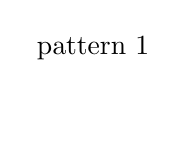
\begin{tikzpicture}
\node [] (n0)  at (0.0,0.0) {};
\node [] (n1)  at (0.0,1.0) {pattern 1}; 
\end{tikzpicture} 
&
\begin{tikzpicture}
\node [] (n1)  at (0.0,2.0) {$T_1 \rightarrow R_1$}; 
\node [] (n2)  at (1.8,1.0) {$T_2 (= R_1) \rightarrow R_3$};
\node [] (n3)  at (4.2,0.0) {$T_3 (= R_2) \rightarrow R_4$}; 

\draw[->] (0.5,1.7) -- (0.5,1.3);
\draw[->] (3.0,0.7) -- (3.0,0.3);


\end{tikzpicture}

\\\hline

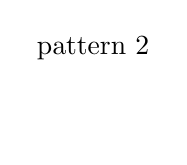
\begin{tikzpicture}
\node [] (n0)  at (0.0,0.0) {};
\node [] (n1)  at (0.0,1.0) {pattern 2}; 
\end{tikzpicture} 
 &
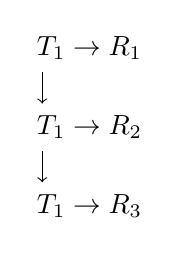
\begin{tikzpicture}
\node [] (n1)  at (0.0,2.0) {$T_1 \rightarrow R_1$}; 
\node [] (n2)  at (0.0,1.0) {$T_1 \rightarrow R_2$};
\node [] (n3)  at (0.0,0.0) {$T_1 \rightarrow R_3$}; 

\draw[->] (-0.6,1.7) -- (-0.6,1.3);
\draw[->] (-0.6,0.7) -- (-0.6,0.3);
\end{tikzpicture}

\\\hline
\begin{tikzpicture}
\node [] (n0)  at (0.0,0.0) {};
\node [] (n1)  at (0.0,2.0) {pattern 3}; 
\end{tikzpicture} 
&
\begin{tikzpicture}
\node [] (n0)  at (2.2,4.0) {$[T]$}; 
\node [] (n1)  at (0.0,3.0) {$T_1 \rightarrow R_1$}; 
\node [] (n2)  at (1.8,2.0) {$T_2 \rightarrow R_2$};
\node [] (n3)  at (4.2,1.0) {$T_3  \rightarrow R_3$}; 

\draw[->] (n0.south) -- (-0.5,3.3);
\draw[->] (n0.south) -- (1.3,2.3);
\draw[->] (n0.south) -- (3.5,1.3);
\end{tikzpicture}

\\\hline

\begin{tikzpicture}
\node [] (n0)  at (0.0,0.0) {};
\node [] (n1)  at (0.0,2.0) {pattern 4}; 
\end{tikzpicture} 
&
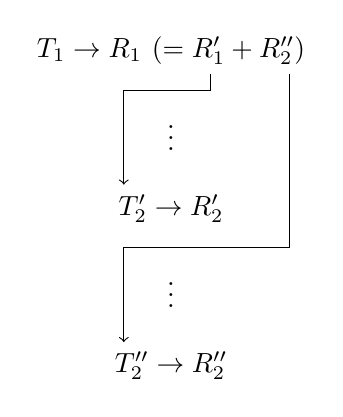
\begin{tikzpicture}
\node [] (n0)  at (0.0,4.0) {$T_1 \rightarrow R_1\textit{ }( = R_1^\prime + R_2^{\prime\prime} )$}; 

\node [] (d0)  at (0.0,3) {$\vdots$}; 

\node [] (n1)  at (0.0,2) {$T_2^\prime \rightarrow R_2^\prime$}; 


\node [] (d0)  at (0.0,1) {$\vdots$}; 


\node [] (n2)  at (0.0,0.0) {$T_2^{\prime\prime} \rightarrow R_2^{\prime\prime}$};

\draw [->] (0.5, 3.7) -- (0.5, 3.5) -- (-0.6, 3.5) -- (-0.6, 2.3);

\draw [->] (1.5, 3.7) -- (1.5, 1.5) -- (-0.6, 1.5) -- (-0.6, 0.3);

\end{tikzpicture}

\end{tabular}
\caption{In the notation used by (?), the horizontal arrow indicates a transition in an utterance, while the vertical one indicates the the contextual connection within of utterances.}
\label{Table:danesh_coherence_patterns}
\end{table}


\newcite{danes74a} interprets the patterns as follows:

\begin{itemize}
\item Pattern 1: A linear transition pattern between themes and rhymes. 
In this pattern, each utterance takes the rhyme presented in the preceding context of the utterance as a given information and transfers it to a new information or a new rhyme. 
In other words, each R (i.e. a new information) becomes the T (i.e. a given information) of the next utterance. 


\item Pattern 2: This pattern depicts a constant theme that continues across utterances. 
One and the same theme appears in a series of utterances. 
Each utterance, however, presents new information about the theme. 


\item Pattern 3: In this pattern $[T]$ indicates a hypertheme that is a global theme of a paragraph or even other text sections. 
 Pattern shows that different utterances can be connected because the themes, or the given information,  of utterances are semantically connected to a hypertheme. 

 \item Pattern 4: 
 \newcite{danes74a} expresses that different combination of these patterns can be employed in different texts. 
 Some of such combinations are so frequent that can be taken as special type of theme-rhyme transition of a higher order. 
  \newcite{danes74a} finds Pattern 4 as one of the most important of such patterns, where an utterance presents two (which can in potential several) rhymes, $R^\prime$ and $R^{\prime\prime}$ , in connection with a given theme. 
  First $R^{\prime}$ expounded and after its progression has been finished, $R^{\prime\prime}$ becomes the theme of another transition. 
  Transitions in between for extending each rhyme follows its own pattern. 
\end{itemize}

\newcite{danes74a} brings this point into attention that one of the important properties of these patterns is omitting links in these patterns.  
For example, in Pattern 1 there is no link between the earliest and latest utterance. 
Those are connected because there is an intermediate utterance that makes transitions between themes and rhymes smoother. 
In contrast, all utterances in Pattern 3  are linked to each other because they all have $T_1$ as a shared given information. 

What \newcite{danes74a} proposed is that the generalized structure of coherent texts may be described in terms of an underlying patterns of transitions between presented themes and rhymes.
This theory is the main motivation of our coherence model in this chapter. 
As before we take entities mentioned in a text as piece of information that make sentences connected. 
The entity graph representation, introduced in Chapter \ref{}, is employed to model the distribution of entities across sentences of a text. 
Then the projection graphs obtained from the entity graph representations of texts model the general structure of sentence node connectivity of texts. 
The entity graph model uses the average ourdegree to encode the connectivity of sentence nodes in projection graphs. 

The main research questions that are investigated in this chapter is:

\begin{itemize}
% \item Is the average outdegree proposed by \newcite{guinaudeau13}  a strong representative metric for the connectivity style of projection graphs and therefore the perceived coherence of texts?
\item Are the any more representative features for the connectivity style of nodes in projection graphs?
\end{itemize}

The idea is to check how well the average outdegree metric models the coherence of a set of well-written articles such as published news articles in Wall Street Journal corpus.  
In spite of this fact that these articles are written by professional authors, human judges assigned to them different range of readability scores (More details in Section \ref{}).  
% We compute the Pearson correlation between the average outdegree of projection graph representations of news articles and their associated score assigned by human judges. 

In order to answer the research question, we employ a subgraph mining algorithm to automatically extract all  subgraphs occurring in projection graphs of these news articles. 
Automatically extracting subgraphs of projection graphs in order to model coherence is our novel contribution in this chapter. 
However, we show that there is a similarity between the automatically mined subgraphs of projection graphs and the coherence patterns proposed by \newcite{danes74a}, indicating that our model's foundation is also linguistically sound.  

We define the frequency of these systematic extracted subgraphs (or coherence patterns) as features that capture the connectivity style of nodes in a projection graph and therefore the coherence property of the corresponding text.  
We evaluate if our novel coherence features outperform the average outdegree feature in a classification task in that more coherent texts should be recognized from less coherent texts. 
In next section, we explain how we exactly model coherence patterns. 


\section{Definitions From Graph Theory}
\label{sec:definition_from_graph_theory}
%
In order to explain the applied subgraphs that encode coherence of sentences in a text, we first need to define some required concepts from graph theory. 

\textbf{Graph.}
A graph is a set of points, we refer to them as nodes, connected by lines, called edges. 
More formally, a graph is a pair of two finite sets $G=( V, E )$ where $V$ is a set of nodes and $E$ is a set of edges whose elements are pairs of nodes. 

\begin{figure}[!ht]
\centering
\small
\begin{tabular}{cc}

	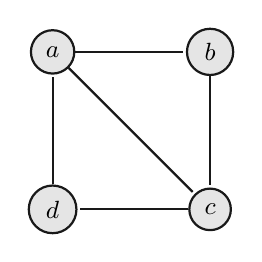
\begin{tikzpicture}[shorten >=1pt,-,scale=0.5]  
		\tikzstyle{node}=[circle,thick,draw=black!90,fill=black!10,minimum size=2mm]
		\tikzstyle{edge}=[draw=black!90, thick]
	   
		 \node [node] (a) at (0,4) {\small{$a$}};
		 \node [node] (b) at (4,4) {\small{$b$}};
		 \node [node] (d) at (0,0) {\small{$d$}}; 
		 \node [node] (c) at (4,0) {\small{$c$}}; 
		 
		 \path[edge] (a) -- (b);
		 \path[edge] (b) -- (c);
		 \path[edge] (c) -- (d);
		 \path[edge] (d) -- (a);
		 \path[edge] (a) -- (c);
       
	\end{tikzpicture}

	&

	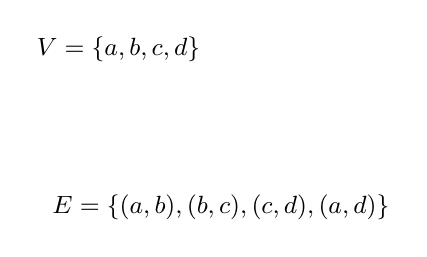
\begin{tikzpicture}[shorten >=1pt,-,scale=0.5]  

		 \node (a) at (0,4) {\small{$V = \left \{ a,b,c,d \right \}$}};
		 \node (b) at (2.6,0) {\small{$E = \left \{(a,b),(b,c),(c,d),(a,d) \right \} $}};

	\end{tikzpicture}

	\\

	$G$ 
	&
	$V:Nodes,E:Edges$ 

\end{tabular}
\caption{Graph. }
\label{fig:graph}
\end{figure} 

If the direction of edges conveys any meaning, then edges can be directed so that for any edge like $e = (x,y)$ the direction is from $x$ towards $y$, which are respectively called the source node and the end node of edge $e$. 
Figure \ref{fig:dir_graph} shows the directed version of the shown graph in Figure \ref{fig:graph}.

\begin{figure}[!ht]
\centering
\small
\begin{tabular}{c}

	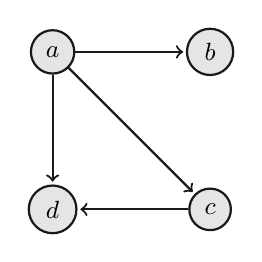
\begin{tikzpicture}[shorten >=1pt,-,scale=0.5]  
		\tikzstyle{node}=[circle,thick,draw=black!90,fill=black!10,minimum size=2mm]
		\tikzstyle{edge}=[draw=black!90, thick]
	   
		 \node [node] (a) at (0,4) {\small{$a$}};
		 \node [node] (b) at (4,4) {\small{$b$}};
		 \node [node] (d) at (0,0) {\small{$d$}}; 
		 \node [node] (c) at (4,0) {\small{$c$}}; 
		 
		 \path[edge,->] (a) -- (b);
		 %\path[edge,->] (b) -- (c);
		 \path[edge,->] (c) -- (d);
		 \path[edge,->] (a) -- (d);
		 \path[edge,->] (a) -- (c);
       
	\end{tikzpicture}
\\

	$G$ 

\end{tabular}
\caption{Directed graph of graph $G$ in Figure \ref{fig:graph}. }
\label{fig:dir_graph}
\end{figure} 


\textbf{Isomorphic.} 
%
Two graphs $G_1$ and $G_2$ are isomorphic, if they fulfill two conditions: (i) a one\--to\--one association, like $f$, exists between nodes of $G_1$ and those of $G_2$, and two nodes of $G_2$ should be connected, if and only if their associated nodes in $G_1$ are connected. 
Figure \ref{fig:isomorphic_graph} illustrates two isomorphic graphs. 
More formally, an isomorphism of graph $G_1$ and $G_2$ is an association between node sets of these graphs:

\begin{equation}
f: V \left( G_1 \right) \rightarrow V \left( G_2 \right),
\end{equation}

such that any  two nodes $u$ and $v$ of $G_1$ are adjacent in $G_1$ if and only if $f \left( u \right)$ and $f \left( v \right)$ are adjacent in $G_2$.
If an isomorphism exists between two graphs, then the graphs are called isomorphic.

\begin{figure}[!ht]
\centering
\small
\begin{tabular}{c@{\hskip 2.5cm}c@{\hskip 2.5cm}c}

	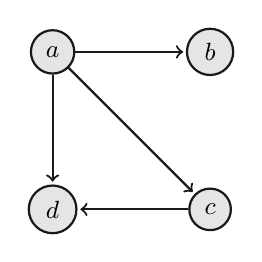
\begin{tikzpicture}[shorten >=1pt,-,scale=0.5]  
		\tikzstyle{node}=[circle,thick,draw=black!90,fill=black!10,minimum size=2mm]
		\tikzstyle{edge}=[draw=black!90, thick]
	   
		 \node [node] (a) at (0,4) {\small{$a$}};
		 \node [node] (b) at (4,4) {\small{$b$}};
		 \node [node] (d) at (0,0) {\small{$d$}}; 
		 \node [node] (c) at (4,0) {\small{$c$}}; 
		 
		 \path[edge,->] (a) -- (b);
		 %\path[edge,->] (b) -- (c);
		 \path[edge,->] (a) -- (c);
		 \path[edge,->] (c) -- (d);
		 \path[edge,->] (a) -- (d);
       
	\end{tikzpicture}

	 &

  	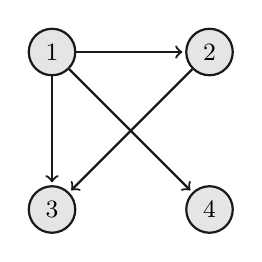
\begin{tikzpicture}[shorten >=1pt,-,scale=0.5]  
	\tikzstyle{node}=[circle,thick,draw=black!90,fill=black!10,minimum size=2mm]
	\tikzstyle{edge}=[draw=black!90, thick]
   
	 \node [node] (1) at (0,4) {\small{$1$}};
	 \node [node] (2) at (4,4) {\small{$2$}};
	 \node [node] (3) at (4,0) {\small{$4$}}; 
	 \node [node] (4) at (0,0) {\small{$3$}}; 
	 
	 \path[edge,->] (1) -- (2);
	 \path[edge,->] (1) -- (3);
	 \path[edge,->] (1) -- (4);
	 \path[edge,->] (2) -- (4);
   
  \end{tikzpicture}

	 &

  	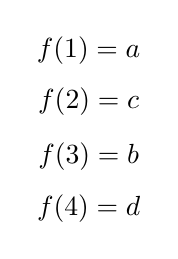
\begin{tikzpicture}[shorten >=1pt,-,scale=0.5]  

	 \node  (1) at (0,4) {$f(1) = a$};
	 \node  (2) at (0,2.7) {$f(2) = c$};
	 \node  (3) at (0,1.3) {$f(3) = b$}; 
	 \node  (4) at (0,0) {$f(4) = d$}; 

  \end{tikzpicture}
\\
$ G_1 $ 
&
 $G_2$
& 
$\textit{Node associations}$

\end{tabular}
\caption{Two isomorphic graphs and a sample association between their nodes. }
\label{fig:isomorphic_graph}
\end{figure} 


\textbf{Subgraph.} 
%
Graph $G_2$ is a subgraph of graph $G_1$, if $G_2$ is isomorphic to a graph whose nodes and edges are a subset of nodes and edges of $G_1$.
\begin{figure}[!ht]
\centering
\small
\begin{tabular}{c@{\hskip 2.5cm}c@{\hskip 2.5cm}c}

	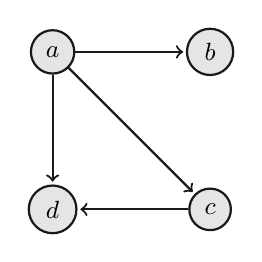
\begin{tikzpicture}[shorten >=1pt,-,scale=0.5]  
		\tikzstyle{node}=[circle,thick,draw=black!90,fill=black!10,minimum size=2mm]
		\tikzstyle{edge}=[draw=black!90, thick]
	   
		 \node [node] (a) at (0,4) {\small{$a$}};
		 \node [node] (b) at (4,4) {\small{$b$}};
		 \node [node] (d) at (0,0) {\small{$d$}}; 
		 \node [node] (c) at (4,0) {\small{$c$}}; 
		 
		 \path[edge,->] (a) -- (b);
		 %\path[edge,->] (b) -- (c);
		 \path[edge,->] (a) -- (c);
		 \path[edge,->] (c) -- (d);
		 \path[edge,->] (a) -- (d);

       
	\end{tikzpicture}

	 &

  	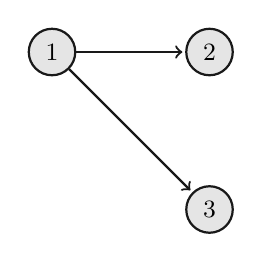
\begin{tikzpicture}[shorten >=1pt,-,scale=0.5]  
	\tikzstyle{node}=[circle,thick,draw=black!90,fill=black!10,minimum size=2mm]
	\tikzstyle{edge}=[draw=black!90, thick]
   
	 \node [node] (1) at (0,4) {\small{$1$}};
	 \node [node] (2) at (4,4) {\small{$2$}};
	 \node [node] (3) at (4,0) {\small{$3$}}; 
	 
	 \path[edge,->] (1) -- (2);
	 \path[edge,->] (1) -- (3);
   
  \end{tikzpicture}

	 &

  	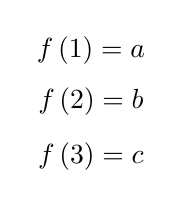
\begin{tikzpicture}[shorten >=1pt,-,scale=0.5]  

	 \node  (1) at (0,4) {$f \left( 1 \right) = a$};
	 \node  (2) at (0,2.7) {$f \left( 2 \right) = b$};
	 \node  (3) at (0,1.3) {$f \left( 3 \right) = c$}; 

  \end{tikzpicture}
\\
$ G_1 $ & $G_2$  & $\textit{Node associations}$

\end{tabular}
\caption{$G_2$ is a subgraphs of graph $G_1$}
\label{fig:subgraph}
\end{figure} 

In the shown example in Figure \ref{fig:subgraph}, graph $G_2$ is isomorphic with graph 

\begin{equation}
G = \left( \left\{ a,b,c \right\}, \left\{ \left( a , b \right),\left( b , c \right) \right\} \right) 
\end{equation}

whose node and edge sets are subsets of node and edge sets of $G_1$.

\textbf{k-node subgraph.}
%
The size of subgraph is the size of its node set that is the number nodes in the graph. 
Graph $G_2 = \left( V_2 , E_2 \right)$ is a k-node subgraph of graph $G_1 = \left( V_1, E_1 \right)$, if $G_2$ is a subgraph of $G_1$, and $V_2$ has $k$ elements, $|V_2|=k$. 
In Figure \ref{fig:subgraph}, graph $G_2$ is a 3-node subgraph of graph $G_1$. 


\textbf{Induced subgraph.} 
%
An induced subgraph of a graph is a subgraph of the graph with an extra condition on its edges.  
That is, in simple words, its edge sets contains all possible edges that are present in the main graph. 
Formally, graph $G_2 = (V_2, E_2)$ is an induced subgraph of graph $G_1 = (V_2, E_2)$ if $V_2 \subseteq V_1$ and 
\begin{equation}
E_2 = \left\{ (x,y)| x \in V_2, y \in V_2, (x,y) \in E_1   \right\}. 
\end{equation}

Figure \ref{fig:induced_subgraphs} shows a graph and two subgraphs of it. 
Subgraph $G_2$ is a subgraph of $G_1$ but not induced, because there is no edge between nodes $1$ and $3$ of this subgraph while their associated nodes, $a$ and $b$, in graph $G_1$ are connected. 
In contrast, subgraph $G_2$ is an induced subgraph of $G_1$ because it contains all possible edges that are present in $G_1$ and connect nodes of the subgraph.  

\begin{figure}[!ht]
\centering
\small
\begin{tabular}{c@{\hskip 1.5cm}c@{\hskip 1.5cm}c@{\hskip 1.5cm}c}

	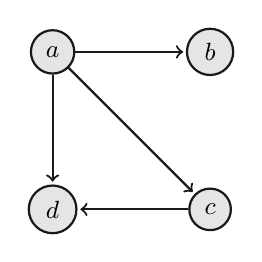
\begin{tikzpicture}[shorten >=1pt,-,scale=0.5]  
		\tikzstyle{node}=[circle,thick,draw=black!90,fill=black!10,minimum size=2mm]
		\tikzstyle{edge}=[draw=black!90, thick]
	   
		 \node [node] (a) at (0,4) {\small{$a$}};
		 \node [node] (b) at (4,4) {\small{$b$}};
		 \node [node] (d) at (0,0) {\small{$d$}}; 
		 \node [node] (c) at (4,0) {\small{$c$}}; 
		 
		 \path[edge,->] (a) -- (b);
		 \path[edge,->] (a) -- (c);
		 \path[edge,->] (c) -- (d);
		 \path[edge,->] (a) -- (d);

       
	\end{tikzpicture}

	 &

  	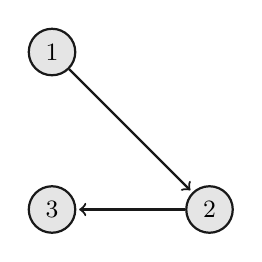
\begin{tikzpicture}[shorten >=1pt,-,scale=0.5]  
	\tikzstyle{node}=[circle,thick,draw=black!90,fill=black!10,minimum size=2mm]
	\tikzstyle{edge}=[draw=black!90, thick]
   
	 \node [node] (1) at (0,4) {\small{$1$}};
	 \node [node] (2) at (4,0) {\small{$2$}};
	 \node [node] (3) at (0,0) {\small{$3$}}; 
	 
	 \path[edge,->] (1) -- (2);
	 \path[edge,->] (2) -- (3);
   
  \end{tikzpicture}

	 &


  	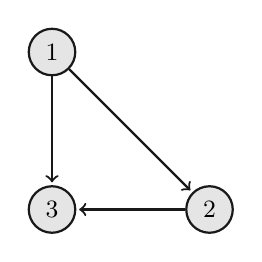
\begin{tikzpicture}[shorten >=1pt,-,scale=0.5]  
	\tikzstyle{node}=[circle,thick,draw=black!90,fill=black!10,minimum size=2mm]
	\tikzstyle{edge}=[draw=black!90, thick]
   
	 \node [node] (1) at (0,4) {\small{$1$}};
	 \node [node] (2) at (4,0) {\small{$2$}};
	 \node [node] (3) at (0,0) {\small{$3$}}; 
	 
	 \path[edge,->] (1) -- (2);
	 \path[edge,->] (2) -- (3);
	 \path[edge,->] (1) -- (3);
   
  \end{tikzpicture}

  &

  	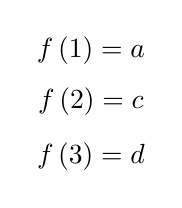
\begin{tikzpicture}[shorten >=1pt,-,scale=0.5]  

	 \node  (1) at (0,4) {$f \left( 1 \right) = a$};
	 \node  (2) at (0,2.7) {$f \left( 2 \right) = c$};
	 \node  (3) at (0,1.3) {$f \left( 3 \right) = d$}; 

  \end{tikzpicture}
\\
$ G_1 $ & $G_2$  & $G_3$ & $\textit{Node associations}$

\end{tabular}
\caption{Induced subgraphs}
\label{fig:induced_subgraphs}
\end{figure} 

It is worth mentioning that henceforth we mean induced subgraphs when using the term subgraph.  
However, in cases that the context is not clear we explicitly distinguish them.     


\textbf{Graph signature.} 
%
Given a list of graphs $ \zeta  = \left[ G_1, G_2, \cdots , G_m \right]$,  a graph signature, which is  denoted by for graph $G$, denoted by $\phi \left( G \right)$,  with respect to $\zeta$ is a vector of frequencies of graphs in $\zeta$ in graph $G$:

\begin{equation}
\phi \left( G \right) = \left( f_1, f_2, f_3, \cdots, f_m \right),
\end{equation}
%
where $f_i$ is the frequency of graphs in graph $G$. 
The frequency of graph $G_i$ in graph $G$ is computed as follows:

\begin{equation}
 f_i = \frac{count(G_i, G)}{\sum_{G_j \in \zeta}{count(G_j, G)}}
\end{equation}
%
where $count(G_i, G)$ is the number of occurrences of $G_i$ in graph $G$. 
The reason of using frequency instead of raw count is that frequency is a normalized value that cannot become biased to the number of nodes and edges of graph $G$. 



\section{Coherence Patterns Modeling}
\label{sec:coherence_patterns_modeling}
%
The entity graph representation of a text encodes the distribution of entities across sentences of a text. 
One-mode projection graphs model the connectivity between sentence nodes with respect to the shared entities between sentences. 
Our main contribution, in this chapter, is that instead of the average outdegree as a simple metric that models the connectivity of sentence nodes of a projection graph, we introduce a set of novel graph-based features that encode the structure of connections (i.e.\ connectivity style) in a projection graph. 
We hypothesize that the frequencies of different subgraphs occurring in projection graphs encode the connectivity style of  projection graphs and therefore, they can be utilized to model coherence.  
Our experiments in Section \ref{} indicate this hypothesis is correct for the examined tasks.  

Given a corpus of documents, we model connections between sentences of each document by its projection graph representation, $P_U$. 
In this step, instead of having a set of documents we have a set of one-mode projection graphs associated with documents. 
We refer to it as the graph set.  
Similar to the entity grid model \cite{barzilay08b}, the key assumption behind our coherence model is that coherent texts reveal similar patterns that differ them from incoherent texts. 
Therefore, the projection graphs of coherent texts reveal similar connectivity style that is different with incoherent texts. 
\newcite{guinaudu13} propose the average outdegree, but we propose to use the graph signature of each projection graph to encode the connectivity style of projection graphs into a vector. 

In order to obtain graph signatures of projection graphs, some basis graphs are required to represent projection graphs based on them. 
We propose to extract all possible subgraphs of projection graphs as basis graphs for computing graph signatures. 

The results of our experiments in Section \ref{}, show that the frequencies of some subgraphs in documents are statistically significantly correlated with scores assigned by human annotators to documents. 
Moreover, as it will be shown in Section \ref{}, some of these subgraphs are similar to what are defined by \newcite{danes74a}. 
Considering these all, we refer to these subgraphs coherence patterns and their frequencies as coherence features.  

Figure \ref{} shows a schema of our idea for extracting coherence patterns and features. 

From the machine learning perspective, the vector representation of the projection graphs can be taken as feature vectors, in which each element is a feature representing one aspect of data. 
These feature vectors can be supplied for training any machine learning model in order to classify coherent documents from incoherent documents. 

\subsection{Subgraph Mining}
\label{subsec:subgraph_mining}
%
Coherence patterns are subgraphs that occur at least in one of projection graphs of documents in a corpus. 
Mining all subgraphs that occur in a graph set is computationally expensive and this problem is proved to be an NP-complete problem \cite{}. 
Intuitively, a graph with $\Vert E \Vert$ edges, potentially has $\mathcal{O} \left( 2^{\Vert E \Vert} \right)$ subgraphs.  
Projection graphs with $\Vert V \Vert$ nodes at most has  $\frac{(n-1)(n-2)}{2}$ that is in order of $\mathcal{O} \left( \Vert V \Vert \right)$.  

In general, the goal of this thesis is not to develop an algorithm for subgraph mining. 
This has been widely studied in computer science and different algorithms and packages have been developed for this. 
The gSpan\footnote{We use the Java package: \url{http://www.cs.ucsb.edu/~xyan/software/gSpan.htm}}  algorithm \cite{yanxifeng02} is one of the efficient methods for mining subgraphs of a  graph set. 
Here, we briefly describe the idea and the method of the gSpan algorithm and refer interested readers to Appendix \ref{} for more details. 

The gSpan,(\textit{g}raph-based \textit{S}ubstructure \textit{pa}ttern \textit{m}ining), algorithm is an approach for extracting all patterns (i.e. subgraphs) that frequently occur in a graph set. 
It discovers all frequent subgraphs without generating the candidates. 
So it is more efficient. 
A subgraph is called frequent if the number of graphs that contain the subgraph is greater than a threshold. 
This threshold is a hyper-parameter of the algorithm\footnote{We always set this threshold to zero to extract all occurring subgraphs in a graph set. We prefer all patterns over frequent patterns because our goal is to investigate .....
 However, is it possible to integrate this in the future work?}.
 gSpan orders graphs in a graph set with respect to their structures and then adapts a depth-first-search search strategy to extract frequent connected subgraphs efficiently. 
 It starts with small subgraphs and simultaneously expands subgraphs and check the frequency of subgraph. 

 [It seems the efficiency of gSpan is when you have a threshold, by setting this to zero it has to extract all possible patterns, so the method is still expensive..]









Subgraph features are divided into two categories: basic subgraphs and frequent large subgraphs.

\textbf{Basic subgraphs.} Instead of frequent subgraphs all possible 3-node subgraphs (Figure \ref{f:all_3node_subgraphs}) are used as
basic subgraphs because they are the smallest meaningful subgraphs that can model coherence patterns. 

Because backward edges never occur in one-mode projections, only four subgraphs are feasible (Figure \ref{f:feasible_3node_subgraphs}).

%\begin{figure}[!ht]
\centering
\resizebox{1.0\columnwidth}{!}{
\begin{tabular}{cccc}
 %%%%%%%%%%%%%%%%%%%%%%%%%%%%%% subgraph 1 %%%%%%%%%%%%%%%%%%%%%%%%%%%%%%
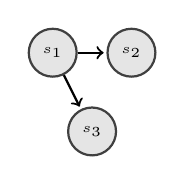
\begin{tikzpicture}[shorten >=1pt,->,scale=0.5]  
        \tikzstyle{sentence}=[circle,thick,draw=black!75,fill=black!10,minimum size=2mm]
        \tikzstyle{edge}=[draw, thick]
       \begin{scope}
         \node [sentence] (s1) at (0,2) {\tiny{$s_1$}};
         \node [sentence] (s2) at (2,2) {\tiny{$s_2$}};
         \node [sentence] (s3) at (1,0) {\tiny{$s_3$}}; 
         \path[edge] (s1) edge [above] node[font=\tiny] {} (s2);
         \path[edge] (s1) edge [above] node[font=\tiny] {} (s3);
        \end{scope}        
      \end{tikzpicture}
&
%%%%%%%%%%%%%%%%%%%%%%%%%%%%%% subgraph 2 %%%%%%%%%%%%%%%%%%%%%%%%%%%%%%
 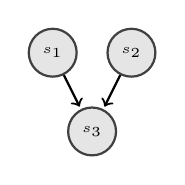
\begin{tikzpicture}[shorten >=1pt,->,scale=0.5]  
        \tikzstyle{sentence}=[circle,thick,draw=black!75,fill=black!10,minimum size=2mm]
        \tikzstyle{edge}=[draw, thick]
       \begin{scope}
         \node [sentence] (s1) at (0,2) {\tiny{$s_1$}};
         \node [sentence] (s2) at (2,2) {\tiny{$s_2$}};
         \node [sentence] (s3) at (1,0) {\tiny{$s_3$}}; 
         \path[edge] (s1) edge [above] node[font=\tiny] {} (s3);
         \path[edge] (s2) edge [above] node[font=\tiny] {} (s3);
        \end{scope}        
      \end{tikzpicture}

&
 %%%%%%%%%%%%%%%%%%%%%%%%%%%%%% subgraph 3 %%%%%%%%%%%%%%%%%%%%%%%%%%%%%%
 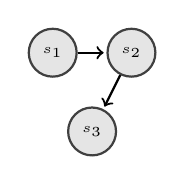
\begin{tikzpicture}[shorten >=1pt,->,scale=0.5]  
        \tikzstyle{sentence}=[circle,thick,draw=black!75,fill=black!10,minimum size=2mm]
        \tikzstyle{edge}=[draw, thick]
       \begin{scope}
         \node [sentence] (s1) at (0,2) {\tiny{$s_1$}};
         \node [sentence] (s2) at (2,2) {\tiny{$s_2$}};
         \node [sentence] (s3) at (1,0) {\tiny{$s_3$}}; 
         \path[edge] (s1) edge [above] node[font=\tiny] {} (s2);
         \path[edge] (s2) edge [above] node[font=\tiny] {} (s3);
        \end{scope}        
      \end{tikzpicture}
      
      
 &
 %%%%%%%%%%%%%%%%%%%%%%%%%%%%%% subgraph 7 %%%%%%%%%%%%%%%%%%%%%%%%%%%%%%
 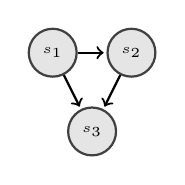
\begin{tikzpicture}[shorten >=1pt,->,scale=0.5]  
        \tikzstyle{sentence}=[circle,thick,draw=black!75,fill=black!10,minimum size=2mm]
        \tikzstyle{edge}=[draw, thick]
       \begin{scope}
        \node [sentence] (s1) at (0,2) {\tiny{$s_1$}};
         \node [sentence] (s2) at (2,2) {\tiny{$s_2$}};
         \node [sentence] (s3) at (1,0) {\tiny{$s_3$}}; 

         
         \path[edge] (s1) edge [above] node[font=\tiny] {} (s2);
         \path[edge] (s1) edge [above] node[font=\tiny] {} (s3);
         \path[edge] (s2) edge [above] node[font=\tiny] {} (s3);
         
        \end{scope}        
      \end{tikzpicture} 
\\

\scriptsize{$sg_1$} & \scriptsize{$sg_2$} & \scriptsize{$sg_3$}& \scriptsize{$sg_4$}
                 

\end{tabular}
}
\caption{Feasible 3\--node subgraph coherence features.}
\label{f:feasible_3node_subgraphs}
\end{figure}

We interpret these subgraphs as follows:

\begin{itemize}
\item \boldmath{$sg_1$}: The connection between a sentence and subsequent ones. In other words, at least two entities are mentioned in one sentence and the subsequent ones are about these entities.

\item \boldmath{$sg_2$}: Indicates that entities in $s_t$ and $s_u$ get connected to each other in $s_v$.

\item \boldmath{$sg_3$}: Each sentence tends to refer to the most prominent entity (focus of attention) in preceding sentences \cite{sidner83,grosz95}. 
The absence of a connection between $s_t$ and $s_v$ indicates that the entity connecting $s_t$ and $s_u$ is different from the entity connecting $s_u$ and $s_v$. 
Therefore this subgraph approximately corresponds to the shift of the focus of attention.

\item \boldmath{$sg_4$}: Merges $sg_1$ and $sg_3$ and represents all connections of these two subgraphs.
\end{itemize}

We use these feasible 3-node subgraphs and compute the graph signature, $\Phi$, of each $G\in\zeta$. 
We propose each $\varphi\in\Phi$ (i.e. relative frequency of each subgraph in $G$) as a connectivity feature of graph $G$ to measure text coherence. 

%\begin{figure}[!ht]
\centering
\small
\resizebox{1.0\columnwidth}{!}{
\begin{tabular}{cccccccc}
 %%%%%%%%%%%%%%%%%%%%%%%%%%%%%% subgraph 1 %%%%%%%%%%%%%%%%%%%%%%%%%%%%%%
\begin{tikzpicture}[shorten >=1pt,->,scale=0.62]  
        \tikzstyle{sentence}=[circle,thick,draw=black!75,fill=black!10,minimum size=2mm]
        \tikzstyle{edge}=[draw, thick]
       \begin{scope}
         \node [sentence] (s1) at (1,2) {\tiny{}};
         \node [sentence] (s2) at (0,0) {\tiny{}};
         \node [sentence] (s3) at (2,0) {\tiny{}}; 
         \path[edge] (s1) edge [above] node[font=\tiny] {} (s2);
         \path[edge] (s1) edge [above] node[font=\tiny] {} (s3);
        \end{scope}        
      \end{tikzpicture}
&
 %%%%%%%%%%%%%%%%%%%%%%%%%%%%%% subgraph 2 %%%%%%%%%%%%%%%%%%%%%%%%%%%%%%
 \begin{tikzpicture}[shorten >=1pt,->,scale=0.62]  
        \tikzstyle{sentence}=[circle,thick,draw=black!75,fill=black!10,minimum size=2mm]
        \tikzstyle{edge}=[draw, thick]
       \begin{scope}
         \node [sentence] (s1) at (0,2) {\tiny{}};
         \node [sentence] (s2) at (2,2) {\tiny{}};
         \node [sentence] (s3) at (1,0) {\tiny{}}; 
         \path[edge] (s1) edge [above] node[font=\tiny] {} (s3);
         \path[edge] (s2) edge [above] node[font=\tiny] {} (s3);
        \end{scope}        
      \end{tikzpicture}

&
 %%%%%%%%%%%%%%%%%%%%%%%%%%%%%% subgraph 3 %%%%%%%%%%%%%%%%%%%%%%%%%%%%%%
 \begin{tikzpicture}[shorten >=1pt,->,scale=0.62]  
        \tikzstyle{sentence}=[circle,thick,draw=black!75,fill=black!10,minimum size=2mm]
        \tikzstyle{edge}=[draw, thick]
       \begin{scope}
         \node [sentence] (s1) at (0,2) {\tiny{}};
         \node [sentence] (s2) at (2,2) {\tiny{}};
         \node [sentence] (s3) at (1,0) {\tiny{}}; 
         \path[edge] (s1) edge [above] node[font=\tiny] {} (s2);
         \path[edge] (s2) edge [above] node[font=\tiny] {} (s3);
        \end{scope}        
      \end{tikzpicture}
      
&
 %%%%%%%%%%%%%%%%%%%%%%%%%%%%%% subgraph 4 %%%%%%%%%%%%%%%%%%%%%%%%%%%%%%
 \begin{tikzpicture}[shorten >=1pt,->,scale=0.62]  
        \tikzstyle{sentence}=[circle,thick,draw=black!75,fill=black!10,minimum size=2mm]
        \tikzstyle{edge}=[draw, thick]
       \begin{scope}
         \node [sentence] (s1) at (0,2) {\tiny{}};
         \node [sentence] (s2) at (2,2) {\tiny{}};
         \node [sentence] (s3) at (1,0) {\tiny{}}; 
         \path[edge] (s1) edge [above] node[font=\tiny] {} (s3);
         \path[edge] (s2) edge [above] node[font=\tiny] {} (s3);
         \path[edge] (s3) edge [above] node[font=\tiny] {} (s2);
         
        \end{scope}        
      \end{tikzpicture}      
      
&
 %%%%%%%%%%%%%%%%%%%%%%%%%%%%%% subgraph 5 %%%%%%%%%%%%%%%%%%%%%%%%%%%%%%
 \begin{tikzpicture}[shorten >=1pt,->,scale=0.62]  
        \tikzstyle{sentence}=[circle,thick,draw=black!75,fill=black!10,minimum size=2mm]
        \tikzstyle{edge}=[draw, thick]
       \begin{scope}
         \node [sentence] (s1) at (1,2) {\tiny{}};
         \node [sentence] (s2) at (0,0) {\tiny{}};
         \node [sentence] (s3) at (2,0) {\tiny{}}; 
         \path[edge] (s2) edge [above] node[font=\tiny] {} (s1);
         \path[edge] (s1) edge [above] node[font=\tiny] {} (s2);
         \path[edge] (s1) edge [above] node[font=\tiny] {} (s3);
         
        \end{scope}        
      \end{tikzpicture}            
      
 &
 %%%%%%%%%%%%%%%%%%%%%%%%%%%%%% subgraph 6 %%%%%%%%%%%%%%%%%%%%%%%%%%%%%%
 \begin{tikzpicture}[shorten >=1pt,->,scale=0.62]  
        \tikzstyle{sentence}=[circle,thick,draw=black!75,fill=black!10,minimum size=2mm]
        \tikzstyle{edge}=[draw, thick]
       \begin{scope}
         \node [sentence] (s1) at (1,2) {\tiny{}};
         \node [sentence] (s2) at (0,0) {\tiny{}};
         \node [sentence] (s3) at (2,0) {\tiny{}}; 
         \path[edge] (s2) edge [above] node[font=\tiny] {} (s1);
         \path[edge] (s1) edge [above] node[font=\tiny] {} (s2);
         \path[edge] (s1) edge [above] node[font=\tiny] {} (s3);
         \path[edge] (s3) edge [above] node[font=\tiny] {} (s1);
         
        \end{scope}        
      \end{tikzpicture}            
      
 &
 %%%%%%%%%%%%%%%%%%%%%%%%%%%%%% subgraph 7 %%%%%%%%%%%%%%%%%%%%%%%%%%%%%%
 \begin{tikzpicture}[shorten >=1pt,->,scale=0.62]  
        \tikzstyle{sentence}=[circle,thick,draw=black!75,fill=black!10,minimum size=2mm]
        \tikzstyle{edge}=[draw, thick]
       \begin{scope}
         \node [sentence] (s1) at (1,2) {\tiny{}};
         \node [sentence] (s2) at (0,0) {\tiny{}};
         \node [sentence] (s3) at (2,0) {\tiny{}}; 
         
         \path[edge] (s1) edge [above] node[font=\tiny] {} (s2);
         \path[edge] (s1) edge [above] node[font=\tiny] {} (s3);
         \path[edge] (s2) edge [above] node[font=\tiny] {} (s3);
         
        \end{scope}        
      \end{tikzpicture}            
      
 &
 %%%%%%%%%%%%%%%%%%%%%%%%%%%%%% subgraph 8 %%%%%%%%%%%%%%%%%%%%%%%%%%%%%%
 \begin{tikzpicture}[shorten >=1pt,->,scale=0.62]  
        \tikzstyle{sentence}=[circle,thick,draw=black!75,fill=black!10,minimum size=2mm]
        \tikzstyle{edge}=[draw, thick]
       \begin{scope}
         \node [sentence] (s1) at (0,2) {\tiny{}};
         \node [sentence] (s2) at (2,2) {\tiny{}};
         \node [sentence] (s3) at (1,0) {\tiny{}}; 
         
         \path[edge] (s2) edge [above] node[font=\tiny] {} (s1);
         \path[edge] (s1) edge [above] node[font=\tiny] {} (s3);
         \path[edge] (s3) edge [above] node[font=\tiny] {} (s2);
         
        \end{scope}        
      \end{tikzpicture}  
\\

&
 %%%%%%%%%%%%%%%%%%%%%%%%%%%%%% subgraph 9 %%%%%%%%%%%%%%%%%%%%%%%%%%%%%%
 \begin{tikzpicture}[shorten >=1pt,->,scale=0.62]  
        \tikzstyle{sentence}=[circle,thick,draw=black!75,fill=black!10,minimum size=2mm]
        \tikzstyle{edge}=[draw, thick]
       \begin{scope}
         \node [sentence] (s1) at (1,2) {\tiny{}};
         \node [sentence] (s2) at (0,0) {\tiny{}};
         \node [sentence] (s3) at (2,0) {\tiny{}}; 
         
         \path[edge] (s1) edge [above] node[font=\tiny] {} (s2);
         \path[edge] (s1) edge [above] node[font=\tiny] {} (s3);
         \path[edge] (s3) edge [above] node[font=\tiny] {} (s2);
         \path[edge] (s2) edge [above] node[font=\tiny] {} (s3);
         
        \end{scope}        
      \end{tikzpicture}             
&
%%%%%%%%%%%%%%%%%%%%%%%%%%%%%% subgraph 10 %%%%%%%%%%%%%%%%%%%%%%%%%%%%%%
 \begin{tikzpicture}[shorten >=1pt,->,scale=0.62]  
        \tikzstyle{sentence}=[circle,thick,draw=black!75,fill=black!10,minimum size=2mm]
        \tikzstyle{edge}=[draw, thick]
       \begin{scope}
         \node [sentence] (s1) at (0,2) {\tiny{}};
         \node [sentence] (s2) at (2,2) {\tiny{}};
         \node [sentence] (s3) at (1,0) {\tiny{}}; 
         
         \path[edge] (s1) edge [above] node[font=\tiny] {} (s2);
         \path[edge] (s2) edge [above] node[font=\tiny] {} (s1);
         \path[edge] (s1) edge [above] node[font=\tiny] {} (s3);
         \path[edge] (s2) edge [above] node[font=\tiny] {} (s3);
         
        \end{scope}        
      \end{tikzpicture}  

 &
 %%%%%%%%%%%%%%%%%%%%%%%%%%%%%% subgraph 11 %%%%%%%%%%%%%%%%%%%%%%%%%%%%%%
 \begin{tikzpicture}[shorten >=1pt,->,scale=0.62]  
        \tikzstyle{sentence}=[circle,thick,draw=black!75,fill=black!10,minimum size=2mm]
        \tikzstyle{edge}=[draw, thick]
       \begin{scope}
         \node [sentence] (s1) at (1,2) {\tiny{}};
         \node [sentence] (s2) at (0,0) {\tiny{}};
         \node [sentence] (s3) at (2,0) {\tiny{}}; 
         
         \path[edge] (s1) edge [above] node[font=\tiny] {} (s2);
         \path[edge] (s1) edge [above] node[font=\tiny] {} (s3);
         \path[edge] (s3) edge [above] node[font=\tiny] {} (s1);
         \path[edge] (s2) edge [above] node[font=\tiny] {} (s3);
         
        \end{scope}        
      \end{tikzpicture}             

&
%%%%%%%%%%%%%%%%%%%%%%%%%%%%%% subgraph 12 %%%%%%%%%%%%%%%%%%%%%%%%%%%%%%
 \begin{tikzpicture}[shorten >=1pt,->,scale=0.62]  
        \tikzstyle{sentence}=[circle,thick,draw=black!75,fill=black!10,minimum size=2mm]
        \tikzstyle{edge}=[draw, thick]
       \begin{scope}
         \node [sentence] (s1) at (0,2) {\tiny{}};
         \node [sentence] (s2) at (2,2) {\tiny{}};
         \node [sentence] (s3) at (1,0) {\tiny{}}; 
         
         \path[edge] (s1) edge [above] node[font=\tiny] {} (s2);
         \path[edge] (s2) edge [above] node[font=\tiny] {} (s1);
         \path[edge] (s1) edge [above] node[font=\tiny] {} (s3);
         \path[edge] (s2) edge [above] node[font=\tiny] {} (s3);
         \path[edge] (s3) edge [above] node[font=\tiny] {} (s2);
         
        \end{scope}        
      \end{tikzpicture}  
&
%%%%%%%%%%%%%%%%%%%%%%%%%%%%%% subgraph 13 %%%%%%%%%%%%%%%%%%%%%%%%%%%%%%
 \begin{tikzpicture}[shorten >=1pt,->,scale=0.62]  
        \tikzstyle{sentence}=[circle,thick,draw=black!75,fill=black!10,minimum size=2mm]
        \tikzstyle{edge}=[draw, thick]
       \begin{scope}
         \node [sentence] (s1) at (1,2) {\tiny{}};
         \node [sentence] (s2) at (0,0) {\tiny{}};
         \node [sentence] (s3) at (2,0) {\tiny{}}; 
         
         \path[edge] (s1) edge [above] node[font=\tiny] {} (s2);
         \path[edge] (s2) edge [above] node[font=\tiny] {} (s1);

         \path[edge] (s2) edge [above] node[font=\tiny] {} (s3);
         \path[edge] (s3) edge [above] node[font=\tiny] {} (s2);
         
         \path[edge] (s1) edge [above] node[font=\tiny] {} (s3);
         \path[edge] (s3) edge [above] node[font=\tiny] {} (s1);
         
        \end{scope}        
      \end{tikzpicture} 
      &
      
\end{tabular}
}
\caption{All possible directed 3\-- node subgraphs.}
\label{f:all_3node_subgraphs}
\end{figure}

\textbf{Frequent large subgraphs.} Since we observe a strong correlation between basic subgraphs and human readability ratings
(Table \ref{t:comp_3node_pearson}), we mine frequent large subgraphs of projection graphs. 
Our intuition is that larger subgraphs are more informative coherence patterns. 
Hence, we extend the coherence features from all feasible 3-node subgraphs to frequent k-node subgraphs. 
We first use an efficient subgraph mining algorithm to extract all subgraphs with size $k$ and then compute the count of each subgraph as an induced subgraph in each graph $G\in\zeta$. 
We retain a subgraph $sg$, if it is frequent (i.e.\ $support(sg)>\lambda$). 
The result of these steps is a two-dimensional matrix whose rows represent graphs in $\zeta$ and columns represent frequent subgraphs with size $k$. 
The cell $\langle G_i,sg_j\rangle$ shows the count of $sg_j$ in graph $G_i$. Given this matrix, we compute the graph signature of each $G\in\zeta$ and take
each element of the graph signature as a coherence feature.




\section{Coherence Modeling}
\label{sec:automatic_extraction}



\section{Experiments}
\label{sec:experiments}

    \subsection{Readability Assessment}
    \label{subsec:readability_assessment}


        Readability depends on many factors which enable readers to process a text. 
        These factors can be used by readability assessment methods to quantify the difficulty of text understanding. 
        Possible applications of readability assessment are automatic text summarization and simplification systems. Measuring readability can also be used in
        question answering and knowledge extraction systems to prune texts with low readability \cite{kate10}.
        
        Many different text features have been used to assess readability. 
        They include shallow features \cite{flesch48,kincaid75}, language modeling features \cite{siluo01,collins-thompson04}, syntactic features \cite{schwarm05} and text flow or coherence \cite{barzilay08,pitler08}. 
        In a coherent text each sentence has some connections with other sentences. 
        Although these local connections make the text more readable, the corresponding coherence features used
        in \newcite{pitler08} (Section \ref{sec:readability_assessment}) are not strongly correlated with human judgments.


            \subsubsection{Data}
            %
            We use the dataset created by \newcite{pitler08} which consists of randomly selected articles from the Wall Street Journal corpus. 
            The articles were rated by three humans on a scale from $1$ to $5$ for readability based on quality measures that are designed to estimate the coherence of articles. The final readability score of each article is the average of these three ratings.
            
            We exclude three files from this dataset: \texttt{wsj\--0382} does not exist in the Penn Treebank \cite{marcus94}\footnote{\newcite{pitler08} also remove one file from their experiments. 
            We assume that it is  \texttt{wsj\--0382}.}. \texttt{wsj\--2090} does not exist in the Penn Discource Treebank \cite{prasad08a}. \texttt{wsj\--1398} is a poem.




% These patterns are encoded as subgraphs in graphs. 
% An advantage is that coherence can be measured beyond simple sentence or node connectivity.  

\subsubsection{Settings}
%



\textbf{Frequent subgraphs.} Since subgraph mining is an NP-complete problem, different algorithms have been introduced to
improve the performance of subgraph mining. 
We use the gSpan\footnote{We use the Java package: \url{http://www.cs.ucsb.edu/~xyan/software/gSpan.htm}} algorithm \cite{yanxifeng02} to mine subgraphs of a graph dataset which contains $P_u^{ER}$ projections. 
An advantage of using efficient subgraph mining algorithms is that we can exhaustively search very large subgraph spaces. 
A graph with $\Vert E \Vert$ edges, however, potentially has $\mathcal{O}(2^{\Vert E \Vert})$ subgraphs. 
Having sparse graphs and using efficient subgraph mining algorithm lets us to search trough this space. 
We mine subgraphs with $k=4$. (Figure \ref{4node_subgraphs}).




%\begin{figure}[!t]
%\centering
\small
\resizebox{1.0\columnwidth}{!}{
%\begin{tabular}{@{\hskip -1ex}c@{\hskip 1ex}c@{\hskip 1ex}c@{\hskip 1ex}c@{}}
\begin{tabular}{cccc}
\scriptsize{$sg_1$} & \scriptsize{$sg_2$} & \scriptsize{$sg_3$} & \scriptsize{$sg_4$}
\\
 %%%%%%%%%%%%%%%%%%%%%%%%%%%%%% sg 1 = 73 %%%%%%%%%%%%%%%%%%%%%%%%%%%%%%
\begin{tikzpicture}[shorten >=1pt,->,scale=0.5]  
        \tikzstyle{sentence}=[circle,thick,draw=black!75,fill=black!10,minimum size=1mm]
        \tikzstyle{edge}=[draw, thick]
       \begin{scope}
         \node [sentence] (s1) at (0,2) {\tiny{$s_1$}};
         \node [sentence] (s2) at (2,2) {\tiny{$s_2$}};
         \node [sentence] (s3) at (2,0) {\tiny{$s_3$}};
         \node [sentence] (s4) at (0,0) {\tiny{$s_4$}};  
         \path[edge] (s1) edge [above] node[font=\tiny] {} (s2);
         \path[edge] (s1) edge [above] node[font=\tiny] {} (s3);
         \path[edge] (s1) edge [above] node[font=\tiny] {} (s4);
         \path[edge] (s2) edge [above] node[font=\tiny] {} (s4);
         \path[edge] (s2) edge [above] node[font=\tiny] {} (s3);
         \path[edge] (s3) edge [above] node[font=\tiny] {} (s4);
        \end{scope}        
      \end{tikzpicture}
&
%%%%%%%%%%%%%%%%%%%%%%%%%%%%%% sg 2 = 74 %%%%%%%%%%%%%%%%%%%%%%%%%%%%%%
\begin{tikzpicture}[shorten >=1pt,->,scale=0.5]  
        \tikzstyle{sentence}=[circle,thick,draw=black!75,fill=black!10,minimum size=2mm]
        \tikzstyle{edge}=[draw, thick]
       \begin{scope}
         \node [sentence] (s1) at (0,2) {\tiny{$s_1$}};
         \node [sentence] (s2) at (2,2) {\tiny{$s_2$}};
         \node [sentence] (s3) at (2,0) {\tiny{$s_3$}};
         \node [sentence] (s4) at (0,0) {\tiny{$s_4$}};  
         \path[edge] (s1) edge [above] node[font=\tiny] {} (s2);
         \path[edge] (s1) edge [above] node[font=\tiny] {} (s3);
         \path[edge] (s1) edge [above] node[font=\tiny] {} (s4);
         \path[edge] (s2) edge [above] node[font=\tiny] {} (s3);
         \path[edge] (s3) edge [above] node[font=\tiny] {} (s4);
        \end{scope}        
      \end{tikzpicture}
&
%%%%%%%%%%%%%%%%%%%%%%%%%%%%%% sg 3 = 83 %%%%%%%%%%%%%%%%%%%%%%%%%%%%%%
\begin{tikzpicture}[shorten >=1pt,->,scale=0.5]  
        \tikzstyle{sentence}=[circle,thick,draw=black!75,fill=black!10,minimum size=2mm]
        \tikzstyle{edge}=[draw, thick]
       \begin{scope}
         \node [sentence] (s1) at (0,2) {\tiny{$s_1$}};
         \node [sentence] (s2) at (2,2) {\tiny{$s_2$}};
         \node [sentence] (s3) at (2,0) {\tiny{$s_3$}};
         \node [sentence] (s4) at (0,0) {\tiny{$s_4$}};  
         \path[edge] (s1) edge [above] node[font=\tiny] {} (s2);
         \path[edge] (s1) edge [above] node[font=\tiny] {} (s3);
         \path[edge] (s2) edge [above] node[font=\tiny] {} (s3);
         \path[edge] (s2) edge [above] node[font=\tiny] {} (s4);
         \path[edge] (s3) edge [above] node[font=\tiny] {} (s4);
        \end{scope}        
      \end{tikzpicture}
&
%%%%%%%%%%%%%%%%%%%%%%%%%%%%%% sg 4 =84 %%%%%%%%%%%%%%%%%%%%%%%%%%%%%%
\begin{tikzpicture}[shorten >=1pt,->,scale=0.5]  
        \tikzstyle{sentence}=[circle,thick,draw=black!75,fill=black!10,minimum size=2mm]
        \tikzstyle{edge}=[draw, thick]
       \begin{scope}
         \node [sentence] (s1) at (0,2) {\tiny{$s_1$}};
         \node [sentence] (s2) at (2,2) {\tiny{$s_2$}};
         \node [sentence] (s3) at (2,0) {\tiny{$s_3$}};
         \node [sentence] (s4) at (0,0) {\tiny{$s_4$}};  
         \path[edge] (s1) edge [above] node[font=\tiny] {} (s2);
         \path[edge] (s1) edge [above] node[font=\tiny] {} (s3);
         \path[edge] (s2) edge [above] node[font=\tiny] {} (s3);
         \path[edge] (s3) edge [above] node[font=\tiny] {} (s4);
        \end{scope}        
      \end{tikzpicture}
\\
\scriptsize{$sg_5$} & \scriptsize{$sg_6$} & \scriptsize{$sg_7$} & \scriptsize{$sg_8$}
\\
%%%%%%%%%%%%%%%%%%%%%%%%%%%%%% sg 5 = 106 %%%%%%%%%%%%%%%%%%%%%%%%%%%%%%
\begin{tikzpicture}[shorten >=1pt,->,scale=0.5]  
        \tikzstyle{sentence}=[circle,thick,draw=black!75,fill=black!10,minimum size=2mm]
        \tikzstyle{edge}=[draw, thick]
       \begin{scope}
         \node [sentence] (s1) at (0,2) {\tiny{$s_1$}};
         \node [sentence] (s2) at (2,2) {\tiny{$s_2$}};
         \node [sentence] (s3) at (2,0) {\tiny{$s_3$}};
         \node [sentence] (s4) at (0,0) {\tiny{$s_4$}};  
         \path[edge] (s1) edge [above] node[font=\tiny] {} (s2);
         \path[edge] (s1) edge [above] node[font=\tiny] {} (s4);
         \path[edge] (s2) edge [above] node[font=\tiny] {} (s3);
         \path[edge] (s2) edge [above] node[font=\tiny] {} (s4);
         \path[edge] (s3) edge [above] node[font=\tiny] {} (s4);
        \end{scope}        
      \end{tikzpicture}
&
%%%%%%%%%%%%%%%%%%%%%%%%%%%%%% sg 6 = 117 %%%%%%%%%%%%%%%%%%%%%%%%%%%%%%
\begin{tikzpicture}[shorten >=1pt,->,scale=0.5]  
        \tikzstyle{sentence}=[circle,thick,draw=black!75,fill=black!10,minimum size=2mm]
        \tikzstyle{edge}=[draw, thick]
       \begin{scope}
         \node [sentence] (s1) at (0,2) {\tiny{$s_1$}};
         \node [sentence] (s2) at (2,2) {\tiny{$s_2$}};
         \node [sentence] (s3) at (2,0) {\tiny{$s_3$}};
         \node [sentence] (s4) at (0,0) {\tiny{$s_4$}};  
         \path[edge] (s1) edge [above] node[font=\tiny] {} (s2);
         \path[edge] (s1) edge [above] node[font=\tiny] {} (s3);
         \path[edge] (s1) edge [above] node[font=\tiny] {} (s4);
         \path[edge] (s2) edge [above] node[font=\tiny] {} (s4);
         \path[edge] (s3) edge [above] node[font=\tiny] {} (s4);

        \end{scope}        
      \end{tikzpicture}
&
%%%%%%%%%%%%%%%%%%%%%%%%%%%%%% sg 7 =126 %%%%%%%%%%%%%%%%%%%%%%%%%%%%%%
\begin{tikzpicture}[shorten >=1pt,->,scale=0.5]  
        \tikzstyle{sentence}=[circle,thick,draw=black!75,fill=black!10,minimum size=2mm]
        \tikzstyle{edge}=[draw, thick]
       \begin{scope}
         \node [sentence] (s1) at (0,2) {\tiny{$s_1$}};
         \node [sentence] (s2) at (2,2) {\tiny{$s_2$}};
         \node [sentence] (s3) at (2,0) {\tiny{$s_3$}};
         \node [sentence] (s4) at (0,0) {\tiny{$s_4$}};  
         \path[edge] (s1) edge [above] node[font=\tiny] {} (s3);
         \path[edge] (s1) edge [above] node[font=\tiny] {} (s4);
         \path[edge] (s2) edge [above] node[font=\tiny] {} (s3);
         \path[edge] (s2) edge [above] node[font=\tiny] {} (s4);
         \path[edge] (s3) edge [above] node[font=\tiny] {} (s4);
        \end{scope}        
      \end{tikzpicture}
&
%%%%%%%%%%%%%%%%%%%%%%%%%%%%%% sg 8 = 127 %%%%%%%%%%%%%%%%%%%%%%%%%%%%%%
\begin{tikzpicture}[shorten >=1pt,->,scale=0.5]  
        \tikzstyle{sentence}=[circle,thick,draw=black!75,fill=black!10,minimum size=2mm]
        \tikzstyle{edge}=[draw, thick]
       \begin{scope}
         \node [sentence] (s1) at (0,2) {\tiny{$s_1$}};
         \node [sentence] (s2) at (2,2) {\tiny{$s_2$}};
         \node [sentence] (s3) at (2,0) {\tiny{$s_3$}};
         \node [sentence] (s4) at (0,0) {\tiny{$s_4$}};  
         \path[edge] (s1) edge [above] node[font=\tiny] {} (s3);
         \path[edge] (s1) edge [above] node[font=\tiny] {} (s4);
         \path[edge] (s2) edge [above] node[font=\tiny] {} (s4);
         \path[edge] (s3) edge [above] node[font=\tiny] {} (s4);
        \end{scope}        
      \end{tikzpicture}
\\
\scriptsize{$sg_9$} & \scriptsize{$sg_{10}$} & \scriptsize{$sg_{11}$} & \scriptsize{$sg_{12}$}
\\


%%%%%%%%%%%%%%%%%%%%%%%%%%%%%% sg 9 =145 %%%%%%%%%%%%%%%%%%%%%%%%%%%%%%
\begin{tikzpicture}[shorten >=1pt,->,scale=0.5]  
        \tikzstyle{sentence}=[circle,thick,draw=black!75,fill=black!10,minimum size=2mm]
        \tikzstyle{edge}=[draw, thick]
       \begin{scope}
         \node [sentence] (s1) at (0,2) {\tiny{$s_1$}};
         \node [sentence] (s2) at (2,2) {\tiny{$s_2$}};
         \node [sentence] (s3) at (2,0) {\tiny{$s_3$}};
         \node [sentence] (s4) at (0,0) {\tiny{$s_4$}};  
         \path[edge] (s1) edge [above] node[font=\tiny] {} (s2);
         \path[edge] (s1) edge [above] node[font=\tiny] {} (s3);
         \path[edge] (s1) edge [above] node[font=\tiny] {} (s4);
         \path[edge] (s2) edge [above] node[font=\tiny] {} (s3);
         \path[edge] (s2) edge [above] node[font=\tiny] {} (s4);
        \end{scope}        
      \end{tikzpicture}
&
%%%%%%%%%%%%%%%%%%%%%%%%%%%%%% sg 10  = 146 %%%%%%%%%%%%%%%%%%%%%%%%%%%%%%
\begin{tikzpicture}[shorten >=1pt,->,scale=0.5]  
        \tikzstyle{sentence}=[circle,thick,draw=black!75,fill=black!10,minimum size=2mm]
        \tikzstyle{edge}=[draw, thick]
       \begin{scope}
         \node [sentence] (s1) at (0,2) {\tiny{$s_1$}};
         \node [sentence] (s2) at (2,2) {\tiny{$s_2$}};
         \node [sentence] (s3) at (2,0) {\tiny{$s_3$}};
         \node [sentence] (s4) at (0,0) {\tiny{$s_4$}};  
         \path[edge] (s1) edge [above] node[font=\tiny] {} (s2);
         \path[edge] (s1) edge [above] node[font=\tiny] {} (s4);
         \path[edge] (s2) edge [above] node[font=\tiny] {} (s3);
         \path[edge] (s2) edge [above] node[font=\tiny] {} (s4);
        \end{scope}        
      \end{tikzpicture}
&
%%%%%%%%%%%%%%%%%%%%%%%%%%%%%% sg 11  = 156 %%%%%%%%%%%%%%%%%%%%%%%%%%%%%%
\begin{tikzpicture}[shorten >=1pt,->,scale=0.5]  
        \tikzstyle{sentence}=[circle,thick,draw=black!75,fill=black!10,minimum size=2mm]
        \tikzstyle{edge}=[draw, thick]
       \begin{scope}
         \node [sentence] (s1) at (0,2) {\tiny{$s_1$}};
         \node [sentence] (s2) at (2,2) {\tiny{$s_2$}};
         \node [sentence] (s3) at (2,0) {\tiny{$s_3$}};
         \node [sentence] (s4) at (0,0) {\tiny{$s_4$}};  
         \path[edge] (s1) edge [above] node[font=\tiny] {} (s4);
         \path[edge] (s2) edge [above] node[font=\tiny] {} (s3);
         \path[edge] (s2) edge [above] node[font=\tiny] {} (s4);
         \path[edge] (s3) edge [above] node[font=\tiny] {} (s4);
        \end{scope}        
      \end{tikzpicture}
&
%%%%%%%%%%%%%%%%%%%%%%%%%%%%%% sg 12 = 165 %%%%%%%%%%%%%%%%%%%%%%%%%%%%%%
\begin{tikzpicture}[shorten >=1pt,->,scale=0.5]  
        \tikzstyle{sentence}=[circle,thick,draw=black!75,fill=black!10,minimum size=2mm]
        \tikzstyle{edge}=[draw, thick]
       \begin{scope}
         \node [sentence] (s1) at (0,2) {\tiny{$s_1$}};
         \node [sentence] (s2) at (2,2) {\tiny{$s_2$}};
         \node [sentence] (s3) at (2,0) {\tiny{$s_3$}};
         \node [sentence] (s4) at (0,0) {\tiny{$s_4$}};  
         \path[edge] (s1) edge [above] node[font=\tiny] {} (s2);
         \path[edge] (s1) edge [above] node[font=\tiny] {} (s3);
         \path[edge] (s1) edge [above] node[font=\tiny] {} (s4);
         \path[edge] (s2) edge [above] node[font=\tiny] {} (s3);
        \end{scope}        
      \end{tikzpicture}
\\
\scriptsize{$sg_{13}$} & \scriptsize{$sg_{14}$} & \scriptsize{$sg_{15}$} & \scriptsize{$sg_{16}$}
\\

%%%%%%%%%%%%%%%%%%%%%%%%%%%%%% sg 13 = 172 %%%%%%%%%%%%%%%%%%%%%%%%%%%%%%
\begin{tikzpicture}[shorten >=1pt,->,scale=0.5]  
        \tikzstyle{sentence}=[circle,thick,draw=black!75,fill=black!10,minimum size=2mm]
        \tikzstyle{edge}=[draw, thick]
       \begin{scope}
         \node [sentence] (s1) at (0,2) {\tiny{$s_1$}};
         \node [sentence] (s2) at (2,2) {\tiny{$s_2$}};
         \node [sentence] (s3) at (2,0) {\tiny{$s_3$}};
         \node [sentence] (s4) at (0,0) {\tiny{$s_4$}};  
         \path[edge] (s1) edge [above] node[font=\tiny] {} (s2);
         \path[edge] (s2) edge [above] node[font=\tiny] {} (s3);
         \path[edge] (s2) edge [above] node[font=\tiny] {} (s4);
         \path[edge] (s3) edge [above] node[font=\tiny] {} (s4);
        \end{scope}        
      \end{tikzpicture}
&
%%%%%%%%%%%%%%%%%%%%%%%%%%%%%% sg 14 =192 %%%%%%%%%%%%%%%%%%%%%%%%%%%%%%
\begin{tikzpicture}[shorten >=1pt,->,scale=0.5]  
        \tikzstyle{sentence}=[circle,thick,draw=black!75,fill=black!10,minimum size=2mm]
        \tikzstyle{edge}=[draw, thick]
       \begin{scope}
         \node [sentence] (s1) at (0,2) {\tiny{$s_1$}};
         \node [sentence] (s2) at (2,2) {\tiny{$s_2$}};
         \node [sentence] (s3) at (2,0) {\tiny{$s_3$}};
         \node [sentence] (s4) at (0,0) {\tiny{$s_4$}};  
         \path[edge] (s1) edge [above] node[font=\tiny] {} (s2);
         \path[edge] (s1) edge [above] node[font=\tiny] {} (s4);
         \path[edge] (s2) edge [above] node[font=\tiny] {} (s3);
         \path[edge] (s3) edge [above] node[font=\tiny] {} (s4);
        \end{scope}        
      \end{tikzpicture}
&
%%%%%%%%%%%%%%%%%%%%%%%%%%%%%% sg 15 =193 %%%%%%%%%%%%%%%%%%%%%%%%%%%%%%
\begin{tikzpicture}[shorten >=1pt,->,scale=0.5]  
        \tikzstyle{sentence}=[circle,thick,draw=black!75,fill=black!10,minimum size=2mm]
        \tikzstyle{edge}=[draw, thick]
       \begin{scope}
         \node [sentence] (s1) at (0,2) {\tiny{$s_1$}};
         \node [sentence] (s2) at (2,2) {\tiny{$s_2$}};
         \node [sentence] (s3) at (2,0) {\tiny{$s_3$}};
         \node [sentence] (s4) at (0,0) {\tiny{$s_4$}};  
         \path[edge] (s1) edge [above] node[font=\tiny] {} (s2);
         \path[edge] (s2) edge [above] node[font=\tiny] {} (s3);
         \path[edge] (s3) edge [above] node[font=\tiny] {} (s4);
        \end{scope}        
      \end{tikzpicture}
&
%%%%%%%%%%%%%%%%%%%%%%%%%%%%%% sg 16 = 216 %%%%%%%%%%%%%%%%%%%%%%%%%%%%%%
\begin{tikzpicture}[shorten >=1pt,->,scale=0.5]  
        \tikzstyle{sentence}=[circle,thick,draw=black!75,fill=black!10,minimum size=2mm]
        \tikzstyle{edge}=[draw, thick]
       \begin{scope}
         \node [sentence] (s1) at (0,2) {\tiny{$s_1$}};
         \node [sentence] (s2) at (2,2) {\tiny{$s_2$}};
         \node [sentence] (s3) at (2,0) {\tiny{$s_3$}};
         \node [sentence] (s4) at (0,0) {\tiny{$s_4$}};  
         \path[edge] (s1) edge [above] node[font=\tiny] {} (s2);
         \path[edge] (s1) edge [above] node[font=\tiny] {} (s3);
         \path[edge] (s2) edge [above] node[font=\tiny] {} (s4);
         \path[edge] (s3) edge [above] node[font=\tiny] {} (s4);
        \end{scope}        
      \end{tikzpicture}
\\
\scriptsize{$sg_{17}$} & \scriptsize{$sg_{18}$} & \scriptsize{$sg_{19}$} & \scriptsize{$sg_{20}$}
\\

%%%%%%%%%%%%%%%%%%%%%%%%%%%%%% sg 17 = 217 %%%%%%%%%%%%%%%%%%%%%%%%%%%%%%
\begin{tikzpicture}[shorten >=1pt,->,scale=0.5]  
        \tikzstyle{sentence}=[circle,thick,draw=black!75,fill=black!10,minimum size=2mm]
        \tikzstyle{edge}=[draw, thick]
       \begin{scope}
         \node [sentence] (s1) at (0,2) {\tiny{$s_1$}};
         \node [sentence] (s2) at (2,2) {\tiny{$s_2$}};
         \node [sentence] (s3) at (2,0) {\tiny{$s_3$}};
         \node [sentence] (s4) at (0,0) {\tiny{$s_4$}};  
         \path[edge] (s1) edge [above] node[font=\tiny] {} (s4);
         \path[edge] (s2) edge [above] node[font=\tiny] {} (s3);
         \path[edge] (s3) edge [above] node[font=\tiny] {} (s4);
        \end{scope}        
      \end{tikzpicture}

&
%%%%%%%%%%%%%%%%%%%%%%%%%%%%%% sg 18 = 227 %%%%%%%%%%%%%%%%%%%%%%%%%%%%%%
\begin{tikzpicture}[shorten >=1pt,->,scale=0.5]  
        \tikzstyle{sentence}=[circle,thick,draw=black!75,fill=black!10,minimum size=2mm]
        \tikzstyle{edge}=[draw, thick]
       \begin{scope}
         \node [sentence] (s1) at (0,2) {\tiny{$s_1$}};
         \node [sentence] (s2) at (2,2) {\tiny{$s_2$}};
         \node [sentence] (s3) at (2,0) {\tiny{$s_3$}};
         \node [sentence] (s4) at (0,0) {\tiny{$s_4$}};  
         \path[edge] (s1) edge [above] node[font=\tiny] {} (s2);
         \path[edge] (s2) edge [above] node[font=\tiny] {} (s3);
         \path[edge] (s2) edge [above] node[font=\tiny] {} (s4);
        \end{scope}        
      \end{tikzpicture}

&
%%%%%%%%%%%%%%%%%%%%%%%%%%%%%% sg 19 =237 %%%%%%%%%%%%%%%%%%%%%%%%%%%%%%
\begin{tikzpicture}[shorten >=1pt,->,scale=0.5]  
        \tikzstyle{sentence}=[circle,thick,draw=black!75,fill=black!10,minimum size=2mm]
        \tikzstyle{edge}=[draw, thick]
       \begin{scope}
         \node [sentence] (s1) at (0,2) {\tiny{$s_1$}};
         \node [sentence] (s2) at (2,2) {\tiny{$s_2$}};
         \node [sentence] (s3) at (2,0) {\tiny{$s_3$}};
         \node [sentence] (s4) at (0,0) {\tiny{$s_4$}};  
         \path[edge] (s1) edge [above] node[font=\tiny] {} (s3);
         \path[edge] (s2) edge [above] node[font=\tiny] {} (s3);
         \path[edge] (s3) edge [above] node[font=\tiny] {} (s4);
        \end{scope}        
      \end{tikzpicture}
&
%%%%%%%%%%%%%%%%%%%%%%%%%%%%%% sg 20 =246 %%%%%%%%%%%%%%%%%%%%%%%%%%%%%%
\begin{tikzpicture}[shorten >=1pt,->,scale=0.5]  
        \tikzstyle{sentence}=[circle,thick,draw=black!75,fill=black!10,minimum size=2mm]
        \tikzstyle{edge}=[draw, thick]
       \begin{scope}
         \node [sentence] (s1) at (0,2) {\tiny{$s_1$}};
         \node [sentence] (s2) at (2,2) {\tiny{$s_2$}};
         \node [sentence] (s3) at (2,0) {\tiny{$s_3$}};
         \node [sentence] (s4) at (0,0) {\tiny{$s_4$}};  
         \path[edge] (s1) edge [above] node[font=\tiny] {} (s3);
         \path[edge] (s1) edge [above] node[font=\tiny] {} (s2);
         \path[edge] (s3) edge [above] node[font=\tiny] {} (s4);
        \end{scope}        
      \end{tikzpicture}
\\
\scriptsize{$sg_{21}$} & \scriptsize{$sg_{22}$} & \scriptsize{$sg_{23}$} & \scriptsize{$sg_{24}$}
\\

%%%%%%%%%%%%%%%%%%%%%%%%%%%%%% sg 21 =277 %%%%%%%%%%%%%%%%%%%%%%%%%%%%%%
\begin{tikzpicture}[shorten >=1pt,->,scale=0.5]  
        \tikzstyle{sentence}=[circle,thick,draw=black!75,fill=black!10,minimum size=2mm]
        \tikzstyle{edge}=[draw, thick]
       \begin{scope}
         \node [sentence] (s1) at (0,2) {\tiny{$s_1$}};
         \node [sentence] (s2) at (2,2) {\tiny{$s_2$}};
         \node [sentence] (s3) at (2,0) {\tiny{$s_3$}};
         \node [sentence] (s4) at (0,0) {\tiny{$s_4$}};  
         \path[edge] (s1) edge [above] node[font=\tiny] {} (s3);
         \path[edge] (s1) edge [above] node[font=\tiny] {} (s4);
         \path[edge] (s2) edge [above] node[font=\tiny] {} (s3);
         \path[edge] (s2) edge [above] node[font=\tiny] {} (s4);
        \end{scope}        
      \end{tikzpicture}
&
%%%%%%%%%%%%%%%%%%%%%%%%%%%%%% sg 22 =278 %%%%%%%%%%%%%%%%%%%%%%%%%%%%%%
\begin{tikzpicture}[shorten >=1pt,->,scale=0.5]  
        \tikzstyle{sentence}=[circle,thick,draw=black!75,fill=black!10,minimum size=2mm]
        \tikzstyle{edge}=[draw, thick]
       \begin{scope}
         \node [sentence] (s1) at (0,2) {\tiny{$s_1$}};
         \node [sentence] (s2) at (2,2) {\tiny{$s_2$}};
         \node [sentence] (s3) at (2,0) {\tiny{$s_3$}};
         \node [sentence] (s4) at (0,0) {\tiny{$s_4$}};  
         \path[edge] (s1) edge [above] node[font=\tiny] {} (s3);
         \path[edge] (s1) edge [above] node[font=\tiny] {} (s4);
         \path[edge] (s2) edge [above] node[font=\tiny] {} (s4);
        \end{scope}        
      \end{tikzpicture}

&
%%%%%%%%%%%%%%%%%%%%%%%%%%%%%% sg 23 = 289  %%%%%%%%%%%%%%%%%%%%%%%%%%%%%%
\begin{tikzpicture}[shorten >=1pt,->,scale=0.5]  
        \tikzstyle{sentence}=[circle,thick,draw=black!75,fill=black!10,minimum size=2mm]
        \tikzstyle{edge}=[draw, thick]
       \begin{scope}
         \node [sentence] (s1) at (0,2) {\tiny{$s_1$}};
         \node [sentence] (s2) at (2,2) {\tiny{$s_2$}};
         \node [sentence] (s3) at (2,0) {\tiny{$s_3$}};
         \node [sentence] (s4) at (0,0) {\tiny{$s_4$}};  
         \path[edge] (s1) edge [above] node[font=\tiny] {} (s4);
         \path[edge] (s2) edge [above] node[font=\tiny] {} (s4);
         \path[edge] (s3) edge [above] node[font=\tiny] {} (s4);
        \end{scope}        
      \end{tikzpicture}

&
%%%%%%%%%%%%%%%%%%%%%%%%%%%%%% sg 24 = 304 %%%%%%%%%%%%%%%%%%%%%%%%%%%%%%
\begin{tikzpicture}[shorten >=1pt,->,scale=0.5]  
        \tikzstyle{sentence}=[circle,thick,draw=black!75,fill=black!10,minimum size=2mm]
        \tikzstyle{edge}=[draw, thick]
       \begin{scope}
         \node [sentence] (s1) at (0,2) {\tiny{$s_1$}};
         \node [sentence] (s2) at (2,2) {\tiny{$s_2$}};
         \node [sentence] (s3) at (2,0) {\tiny{$s_3$}};
         \node [sentence] (s4) at (0,0) {\tiny{$s_4$}};  
         \path[edge] (s1) edge [above] node[font=\tiny] {} (s2);
         \path[edge] (s1) edge [above] node[font=\tiny] {} (s3);
         \path[edge] (s1) edge [above] node[font=\tiny] {} (s4);
        \end{scope}        
      \end{tikzpicture}



\end{tabular}
}

%\caption{Frequent subgraphs with four nodes where $t<u<v<w$.}\label{4node_subgraphs}
%\end{figure}


%



\subsubsection{Results}\label{subsec:results}
%
\textbf{Readability assessment.}  
\noindent
\textbf{Readability assessment.} We use the Pearson correlation coefficient to find features correlated with readability scores. 
It takes feature values and readability scores of all articles and returns $-1\leq\rho\leq+1$. 
A high value of $|\rho|$ shows a strong correlation. 
We report statistical significance on the $0.05$-level. 
We report the correlation of our coherence models encoded in graph features and compare them with \newcite{guinaudeau13} entity graph as the state-of-the-art coherence model. 
\newcite{pitler08} show that the entity transition features extracted from the entity grid model \cite{barzilay08} on its own do not significantly predict human
readability ratings. 
So we do not describe their results here.

\begin{table}[!t]
\centering
\begin{small}
\begin{tabular}{lrc}
\hline
                        & $\rho$                & p\_value\\\hline
        \multicolumn{3}{l}{\textbf{Entity Graph}}\\
 $P_u^{ER}$             & $-0.013$ & 0.949 \\
 $P_w^{ER}$             & 0.151  & 0.452\\
 $P_{acc}^{ER}$ & 0.150         & 0.455\\
\hline
\multicolumn{3}{l}{\textbf{Discourse Relation Graph}}\\
 $P_u^{DR}$ &  0.150 & 0.455\\
 $P_w^{DR}$ &  0.155  & 0.440\\\hline
 \multicolumn{3}{l}{\textbf{Combination of Entity and Discourse Relation}}\\
 $P_u^{ER} \lor P_u^{DR}$  &  0.083 & 0.681\\
 $P_w^{ER} + P_u^{DR}$ & 0.185  & 0.356\\
 $P_w^{ER} + P_w^{DR}$ & 0.187  & 0.350\\\hline
\end{tabular}
\end{small}
\caption{The correlation of the average outdegree of different graphs with human readability ratings.}
  \label{t:OD_pearson}
\end{table}

The results for the outdegree feature is shown in Table \ref{t:OD_pearson}.
% The first section of the table shows the correlation of outdegree feature of three kinds of projections of the entity graph model. 
The average outdegree of $P_w^{ER}$ is highly correlated with human readability ratings. This confirms the readability results of
\newcite{guinaudeau13} on the Encyclopedia Britannica dataset. 
% The second section shows the correlation of the outdegree of unweighted $P_u^{DR}$ and weighted $P_w^{DR}$ discourse relation graphs. 
The outdegrees of discourse relation graphs are more strongly correlated with human readability ratings than the outdegree of the projections in the entity graph, suggesting that efficient graph-based encoding of discourse relations can measure readability well.
% The last section shows the result of the correlation of different combined graphs' outdegree. 
The outdegree of the combined graph $P_w^{ER}+P_w^{DR}$ is highly correlated, showing that the interaction of entity connections and discourse relations is important for text coherence.
% Moreover, getting higher correlation coefficient with combined graphs than the projections of entity graph and discourse relations graphs, saying that the entity graph model needs to enrich with semantical continuity relations and our combined models merge the entity graph with discourse relations as logical connections in a text. On the other hand
However, none of the outdegree measures in this table are significantly correlated with human readability ratings, confirming the intuition that outdegree only measures node connectivity in graphs and it is not enough to measure readability.

\begin{table}[!h]
\centering
\begin{small}
\begin{tabular}{lrc}
\hline
   & $\rho$ & p\_value\\\hline
\textbf{Number of Components}   &       $\mathbf{-0.391}$       &       \textbf{0.044}  \\\hline

\multicolumn{3}{l}{\textbf{Relative frequency of 3-node Subgraphs}} \\
 $sg_1$ &  0.310 & 0.116\\
 $sg_2$ & $-0.325$ & 0.098\\
$\mathbf{sg_3}$ & $\mathbf{-0.384}$ & \textbf{0.048}\\
 $sg_4$ &  0.108 & 0.592\\\hline
\end{tabular}
\end{small}
\caption{Number of components and subgraph $sg_3$ are significantly correlated to readability.}
  \label{t:comp_3node_pearson}
\end{table}

Table \ref{t:comp_3node_pearson} shows the correlation of two features of projections\footnote{Although, the proposed features can be applied on all kind of presented graphs, we evaluate them (except outdegree) only on projections of the entity graph model. 
We leave the application to the other graph representations for future work.}:
The number of components has a strong and significant negative correlation with human readability ratings\footnote{This supports
  \newcite{karamanis09} who report that NOCB transitions in the centering model can be used for the sentence ordering task.},
suggesting that simple properties of graphs measure text
coherence. 
The lower part of Table \ref{t:comp_3node_pearson} shows the correlation of the relative frequency of 3-node subgraphs (see Figure \ref{f:feasible_3node_subgraphs}).  
More readable articles have many $sg_1$ and few number of $sg_2$ patterns. 
Pattern $sg_3$ is significantly and negatively correlated with human readability judgments, confirming the intuition that many shifts in focus
of attention make texts difficult to read. 



\begin{table}[!t]
\centering
\begin{small}
\begin{tabular}{lcrc}
\hline
   & number of edges & $\rho$ & p\_value\\\hline
$sg_1$ & 6 & 0.103 & 0.609   \\
$sg_2$ & 5 & $-0.212$ & 0.288    \\
$sg_3$  & 5 &   $-0.176$ & 0.380      \\
$sg_4$  & 4 &$-0.257$ & 0.196    \\
$sg_5$ & 5 &$-0.140$ & 0. 486   \\
$sg_6$  & 5 &   0.200 &  0.317  \\
$\mathbf{sg_7}$ & \textbf{5} & $\mathbf{-0.402}$ & \textbf{0.038}  \\
$sg_8$  & 4 &$-0.317$ & 0.107 \\
$sg_9$ & 5 & 0.153 & 0.446   \\
$sg_{10}$ & 4 & $-0.238$ & 0.232    \\
$\mathbf{sg_{11}}$ & \textbf{4} & $\mathbf{-0.509}$     & \textbf{0.007}\\
$\mathbf{sg_{12}}$  & \textbf{4} &\textbf{0.449} & \textbf{0.019}    \\
$sg_{13}$  & 4 & $-0.045$ & 0.824    \\
$sg_{14}$ & 4 & $-0.033$ & 0.870\\
$sg_{15}$ & 3 &$-0.358$ & 0.067    \\
$sg_{16}$ &     4 &$-0.068$ & 0.736    \\
$sg_{17}$  & 3 & $-0.308$ & 0.118    \\
$\mathbf{sg_{18}}$ & \textbf{3} & $\mathbf{-0.546}$      & \textbf{0.003}   \\
$\mathbf{sg_{19}}$ & \textbf{3} & $\mathbf{-0.601}$ & \textbf{0.001}   \\
$sg_{20}$ & 3 & 0.094   & 0.641 \\
$sg_{21}$  & 4 & 0.068 & 0.736   \\
$sg_{22}$ &  3& $-0.374$ &  0.055  \\
$sg_{23}$ &     3&$-0.314$ & 0.111 \\
$sg_{24}$ &     3& 0.100 & 0.620  \\
\hline
\end{tabular}
\end{small}
\caption{The correlation between the relative frequency of 4-node subgraphs and readability ratings.}\label{t:correlation_4node_subgraph}
\end{table}


Table \ref{t:correlation_4node_subgraph} shows the correlation between the relative frequency of 4-node subgraphs and readability ratings. 
First, most subgraphs with less than four edges are negatively correlated with readability, except $sg_{20}$ and $sg_{24}$ which are weakly correlated with readability. Few connections between sentences make the text difficult to read.

Second, the highest positive and significant correlation of $sg_{12}$ and the most negatively correlated subgraph $sg_{11}$ show that different patterns of edges in subgraphs capture readability judgments. 
\newcite[p.29]{stoddard91} explains this by the \emph{ambiguity node}\ phenomenon: ``[...] in some cases, there may be more
than one logical, possible node for a given cohesive element in a text, in which case, a reader may see the resulting ambiguity but not be able to decide between the choices''. 
E.g., in $sg_{11}$ a reader may make a decision about the focus of attention in $s_w$, while in $sg_{12}$ the focus of attention of $s_w$ is the same as the
focus of attention of $s_t$. This phenomenon can also be observed in all positively correlated subgraphs. If readers have to return to one point in the text, they prefer to return to a sentence which is the core of the preceding sentences.
% Of course, it is difficult to interpret these patterns one by one, since in a graph they can occur  in different situations. But these analysis show that humans easily understand texts which contain many number of pattern $sg_{12}$.
However, we should refrain of interpreting too much into these patterns.

Finally, we conclude that in all strongly negative correlated subgraphs, a subgraph suffers either from edge shortage or the \textit{ambiguity node}\ phenomenon like $sg_7$.

Considering the correlation of 3-node subgraphs in Table \ref{t:comp_3node_pearson} and 4-node subgraphs in Table \ref{t:correlation_4node_subgraph}, two results are noticeable.
First, in large subgraphs there are more strongly correlated subgraphs than 3-node subgraphs, confirming our hypothesis that larger subgraphs convey coherence patterns with higher quality. Second, $sg_{12}$ in 4-node subgraphs is more strongly and positively correlated than $sg_4$ in 3-node subgraphs, because $sg_{12}$ captures more circumstances about $s_t$. 
The relative frequency of $sg_{12}$ is more informative than $sg_4$'s relative frequency.

\noindent
\textbf{Readability as ranking.} 

\textbf{Readability as ranking.} We rank texts pairwise with respect to their readability. 
We define a classification problem with a set of text pairs and a label, which indicates whether the first text in a pair is more readable. 
We use every two texts whose human readability scores differ by at least $0.5$. 
Each text is represented with its graph-based coherence features. 
We employ WEKA's linear support vector implementation (SMO)  to classify the pairs. 
Performance is evaluated using 10-fold cross-validation.

Results of the readability ranking problem are shown in Table \ref{t:classification_task}. 
Baseline features are entity transition features which are used as coherence features by \newcite{pitler08}\footnote{The accuracy reported in their paper is $79.42\%$. Our reimplementation achieves higher accuracy, because our dataset has three articles less.}.

\begin{table}[!h]
\centering
\begin{small}
\begin{tabular}{@{}lc@{}}
\hline
\textbf{Features} & \textbf{Accuracy} \\\hline
\multicolumn{2}{l}{\textbf{Baselines}} \\
None (Majority class) & 47.85\% \\
Baseline features \cite{pitler08} & 83.25\% \\\hline
\multicolumn{2}{l}{\textbf{Graph-based Features}} \\
Number of components & 61.72\%\\
Basic subgraphs (3-node) & 79.43\% \\
Frequent large subgraphs (4-node) & 89.00\%  \\
Frequent basic + large subgraphs & 88.52\% \\
Baseline features + frequent large subgraphs & 93.30\% \\
\hline
\end{tabular}
\end{small}
\caption{SVM prediction accuracy.}\label{t:classification_task}
\end{table}

When classifying with graph signatures based on basic subgraphs, accuracy is lower than with the baseline coherence features. 
This is probably related to the entity grid features which represent grammatical role transitions of entities, while the basic subgraphs only models the occurrence of entities across sentences. 
Graph signatures based on large subgraphs improve the performance of basic subgraphs by around 10\%. 
This high accuracy verifies that larger subgraphs capture coherence patterns with high quality. 
Combining basic (3-node) and large subgraphs (4-node) cannot improve the performance of the large subgraphs features. 
This probably is because basic subgraphs are implicitly included in larger subgraphs. 
The combination of coherence baseline features and frequent large subgraphs improves the accuracy.



%This idea that each word in a text will be considered a cohesive ties is introduced in \newcite{stoddard91}. 
% \newcite{stoddard91} in her analysis expresses that designing a research package for analyzing of  cohesion patterns is complicated because of different number of cohesive ties, the number of evaluated written texts by human readers. 
% The narrowing can be done in any one or several ways. 
% One is the selection of the type of cohesion ties to be analyzed. 
% The second is the selection of the corpus. 
% Following our entity-based setting in previous chapters, we limit our cohesive ties are restricted version of references in \newcite{halliday76}, the string match between nouns. 
% If, however, a writer chooses to simply repeat nodes without using many cohesive elements, we might expect that readers would find  the content equally cohesive (but probably boring for its repetitiveness).
% There would be a relationship between the phenomenon of node repetition and memory retention \cite{stoddard91}. 
%Certainly, cohesive ties that span sentence and paragraph boundaries have greater potential for unifying a text and making it more cohesive. 

\subsection{Automatic Summarization}
\label{subsec:automatic_summarization}

The growth in the scientific output of many different fields makes the task of automatic summarization imperative. 
Automatic summarizers assist researchers to have an informative and coherent gist of long scientific articles. 
An automatic summarizer produces summaries considering three properties: Importance: The summary should contain the important information of the input document. 
Non-redundancy: The summary should contain non-redundant information. 
The information should be diverse in the summary.
Coherence: Though the summary should comprise diverse and important information of the input document, its sentences should be connected to one another such that it becomes coherent and easy to read. 

If we do not ensure that a summary is coherent, its sentences may not be properly connected. 
This results in an obscure summary. 
In previous work coherence has not been thoroughly considered. 
Parveen and Strube (2015) use single sentence connectivity in the input document as a coherence measure. 
They measure coherence by calculating the outdegree of a sentence in a graph representation of an input document. 
This has two disadvantages: first, since it is computed only based on one sentence, it is not sufficient to generate coherent summaries; second, it is obtained based on sentence connectivity in the input document rather than in the summary. 


In this section, we focus on the coherence aspect of summarization. 
We use discourse entities as the unit of information that relate sentences. 
Here, discourse entities are referred to as head nouns of noun phrases (see Section 2). 
The main goal is to extract sentences which refer to those entities which are important and unique, and also to entities which connect the extracted sentences in a coherent manner. 
Entities in connected sentences can be used to create linguistically motivated coherence patterns (Danes?, 1974). 
Recently, Mesgar and Strube (2015) modeled these coherence patterns by subgraphs of the graph representation (nodes represent sentences and edges rep- resent entity connections among sentences) of documents. 
They show that the frequency of coherence patterns can be used as features for coherence.


The key idea of this paper is to apply coherence patterns to long scientific articles to extract (possibly) non-adjacent sentences which, however, are already coherent. 
Based on the assumption that abstracts of scientific articles are similar in style to coherent summaries, we obtain coherence patterns by analyzing a corpus of abstracts of articles from bio- medicine (PubMed corpus). 
Then we apply the most frequent coherence patterns to input documents, i.e. long scientific articles from bio-medicine (PLOS Medicine dataset), extract corresponding sentences to generate coherent summaries, and evaluate them by comparing with summaries written by a PLOS Medicine editor. 
Figure 1 illustrates the extraction of sentences from an input document (Figure 1, (ii)) which constitute a coherence pattern (Figure 1, (i)).  
If we overlay the input document with coherence patterns and extract the sentences which constitute those patterns, then the extracted sentences are al- ready coherent. We also take into account importance and non-redundancy. We capture all three factors in an objective function maximized by Mixed Integer Programming (MIP).

\textbf{Mining Coherence Patterns}
We use one-mode projection graphs of abstracts in the PubMed corpus (see Section 3.1) to mine coherence patterns. 
The weight of a coherence pattern, weight(patu), is its frequency in the PubMed corpus normalized by the maximum number of its occurrence in abstracts in the PubMed corpus (Equation 1). 

\begin{equation}
weight(pat_u) = \frac{\sum_{k=1}^{q}{freq(pat_u,g_k)}}{max_{k=1}{q}{freq(pat_u,g_k)}}
\end{equation}

where $q$ is the number of graphs associated with abstracts in the corpus, and gk represents the graph of the $k^{th}$ abstract in the PubMed corpus.
The weights of the coherence patterns are not on the same scale. 
We normalize the weights using the standard score  $\frac{x-\mu}{\sigma}$, where ? is the mean and ? is the standard deviation. 
A sigmoid function scales weights to the interval [0, 1].


\textbf{Summary Generation}
We maximize importance, non-redundancy and pattern-based coherence with their respective weights $?$ to generate coherent summaries. 
The objective function is:
$\max(?_I f_I(S) + ?_Rf_R(E) + ?_C f_C(P ))$

where $S$ is a set of binary variables for sentences in an article, $E$ is a set of binary variables for entities and $P$ is a set of binary variables for coherence patterns.

Importance $(f_I(S))$: The importance function quantifies the overall importance of information in the summary, which is calculated by considering the ranks of selected sentences for the summary:

\begin{equation}
f_I(S) = \sum_{i=1}^{n}{Rank(sent_i) \dot s_i}
\end{equation}

In Equation 3, $Rank(sent)$ represents the rank of sentence $sent_i$ and $s_i$ is the binary variable of sentence $sent_i$. $n$ is the number of sentences. 
Kleinberg (1999) develops the Hubs and Authorities algorithm (HITS) to rank web pages. 
He divides web pages into two sets: Hubs, pages which contain links to informative web pages, and Authorities, informative web pages. Here, Hubs are entities and Authorities are sentences. 
We calculate the rank of sentences using the HITS algorithm (Parveen and Strube, 2015). 
Initial ranks for sentences and entities are computed by Equations 4 and 5 in an entity graph:

\begin{equation}
Rank_{init}(sent_i)= 1+ sim{sent_i,title}
\end{equation}
\begin{equation}
Rank_{init}(ent_j)= 1
\end{equation}

In Equation 4, $sim(sent_i,title)$ is the cosine similarity between the scientific article?s title and sentence $sent_i$. 
In Equation 5, $ent_j$ refers to the $j_th$ entity in the entity graph. 
After applying the HITS algorithm on the entity graph using the above initialization, the final rank of a sentence is its importance.

\textbf{Non-redundancy ($f_R(E)$):} In the objective function, $f_R(E)$ represents the non-redundancy of information in the summary. Intuitively, if the summary has unique information in every sentence then the summary is non-redundant. 
We measure non- redundancy as follows:

\begin{equation}
f_R(E) = \sum_{j=1}^{m}{e_j}
\end{equation}

where $m$ is the number of entities and $e_j$ is a binary variable for each entity. 
The summary becomes non-redundant if we include only unique entities. 
On the basis of $f_I(S)$ and $f_R(E)$ we define the following optimization constraints:
\begin{equation}
\sum_{i=1}^{n} |sent_i|.s_i \le l_{max}
\end{equation}

\begin{equation}
\sum_{j\in E_i} {e_j  \ge |E_i|.s_i} for i = 1,...,n
\end{equation}

\begin{equation}
\sum_{s_i \in S_j}{s_i \ge e_j} for j = 1,...,m
\end{equation}

The constraint in Equation 7 limits the length of the summary. 
$l_max$ is the maximal length of the summary and $|sent_i|$ is the length of sentence $sent_i$.

In Equation 8, the constraint ensures that if sentence $sent_i$ is selected $(si = 1)$, then all entities $E_i$ present in sentence $sent_i$ must also be selected. 
In Equation 9, $S_j$ represents the set of binary variables of sentences which contain entity $ent_j$. 
This constraint prescribes that if entity $ent_j$ is selected $(ej = 1)$, then at least one of the sentences in $S_j$ must be selected, too.

Coherence $(f_C(P))$: We use the mined patterns to extract sentences from the input document of PLOS Medicine to create a coherent summary. 
We extract sentences, if the connectivity among nodes in their projection graph matches the connectivity among nodes in a coherence pattern. 
In Figure 3 we overlay the projection graph from Figure 2, ii with the coherence pattern from Figure 1, i. 
This results in three instances of this coherence pattern. 
However, we select only one since we simultaneously optimize for importance and non-redundancy. 

In the objective function, $f_C(P )$ measures the coherence of the summary based on the weights of the coherence patterns occurring in it (Section 2.2):

\begin{equation}
f_C(P) = \sum_{u=1}^{U}{weight(pat_u) \dot p_u}
\end{equation}
where $p_u$ is a boolean variable associated with coherence pattern $pat_u$ .

% Let $P$ be the set of boolean variables of the coherence patterns. 
The optimization considers pattern $pat_{u}$ for summarizing the input article, if $pat_{u}$ is a subgraph of the projection graph of the article. To find the coherence pattern in a projection graph we apply a graph matching algorithm \cite{lerouge15}.
% This algorithm uses Integer Linear Programming (ILP) to ensure whether the given graph matches a subgraph of another graph \cite{lerouge15}.

%\begin{figure}[!ht]
%\begin{center}
%     \includegraphics[scale=0.15]{figures/drawing1.pdf}
%
%    \caption{An illustration of mapping variables to overlay graph $g$ with coherence pattern $pat_u$.}
%     % \ref{fig:entity_grid}}  
%    \label{fig:Map_Var}
%
%\end{center}
%  %\end{justifying}
%\end{figure}

% We want to incorporate coherence patterns as a coherence measure, and build a model which tightly connects coherence, non-redundancy and importance.
% To achieve this, we deal with the graph matching problem.
To model the graph matching problem between projection graph $g=(V_{g},E_{g})$ and patterns $pat_{u}=(V_{pat_{u}},E_{pat_{u}})$, two kinds of mapping binary variables are used: $x_{i,k}$ for the node map, and $y_{ij,kl}$ for the edge map. $x_{i,k,}=1$, if vertices $i\in V_{pat_{u}}$ and $k\in V_g$ match. $y_{ij,kl}=1$, if for each pair of edges $ij \in E_{pat_{u}}$ and $kl \in E_g$ match (Figure \ref{fig:Map_Var}).
% illustrates these matching variables. 
Constraints for graph matching are as follows:

\begin{itemize}
%
\item Every node of the pattern matches at most one unique node of the graph:
\begin{equation}
\sum_{k\in V_g}x_{i,k} \leq 1 \quad \forall i\in V_{pat_{u}}
\end{equation}
%
\item Every edge of the pattern matches at most one unique edge of the graph:
\begin{equation}
\sum_{kl\in E_g}y_{ij,kl} \leq 1 \quad \forall ij\in E_{pat_{u}}
\end{equation}
%
\item Every node of the graph matches at most one node of the pattern:
\begin{equation}
\sum_{i\in V_{pat_{u}}}x_{i,k} \leq 1 \quad \forall k\in V_g
\end{equation}
%
\item A node of pattern $pat_u$ matches a node of graph $g$ if an edge originating from the node of $pat_u$ matches an edge originating from the node of $g$:
\begin{multline}
\hspace{-2em}
\sum_{kl\in E_g}y_{ij,kl} =  x_{i,k} \; \forall k\in V_g, \forall ij\in E_{pat_{u}}
\end{multline}
%
\item A node of pattern $pat_u$ matches a node of graph $g$ if an edge targeting the node of $pat_u$ matches an edge targeting the node of $g$:
%
\begin{multline}
\hspace{-2em}
\sum_{kl\in E_g}y_{ij,kl} =  x_{j,l} \; \forall l\in V_g, \forall ij\in E_{pat_{u}}
\end{multline}
%
\item We need a constraint to extract \emph{induced} patterns\footnote{Pattern $pat_{u}$ is an induced subgraph of graph $g$ if $pat_{u}$ contains all possible edges which appear in $g$.}:
\begin{multline}
\sum_{i\in V_{pat_{u}}}x_{i,k} + \sum_{j \in V_{pat_{u}}}x_{j,l} \\- \sum_{ij\in E_{pat_{u}}}y_{ij,kl} \leq 1
 \quad \forall kl\in E_g
\end{multline}
\end{itemize}

Constraints in Equations $11-16$ are defined to find pattern $pat_u$ in projection graph $g$ of the input article. However these constraints do not ensure that the pattern is in the summary.
% In other words, the nodes corresponding to the sentences selected for the summary constitute the pattern or not. 
For this, we define constraints in Equations $17-19$ to assure that an existing pattern in an article is selected if there are some sentences in the summary which constitute the pattern.

\begin{itemize}

\item Constraint in Equation $17$ ensures that if sentences $s_{k}$ and $s_{l}$ are selected for the summary then the edge between them is selected $(z_{kl}=1)$, too.
\begin{equation}
 s_{k} \cdot s_{l}=z_{kl} \quad \forall k,l \in V_{g}
\end{equation}
%
%\item The pattern $p_{u}$ is selected if it contains the sentences which are selected for a summary i.e. if $s_{k}=1$ and node $k$ is mapped with a pattern node $i$ and $z_{k,l}=1$ and edge $k,l$ is mapped with $i,j$ then $p_{u}=1$. 
%The constraint is shown below:
%\begin{itemize}
\item Pattern $pat_u$ is present in the summary ($p_u=1$) if and only if
% meets two conditions. First, $pat_u$ has to be a subgraph of the projection graph of the input document, i.e., $x_{i,k,pat_{u}}=1$, and $y_{ij,kl,pat_{u}}=1$. Second, 
% the connectivity structure among 
% some of the selected sentence nodes match $pat_u$, i.e., $s_{k}=1$, and $z_{kl}=1$. 
one of its instances in the projection graph is included in the summary, i.e., some of the selected sentence nodes must be present in an instance of pattern $pat_{u}$.
$|V_{pat_{u}}|$ is the number of nodes in pattern $pat_{u}$, and $|E_{pat_{u}}|$ is the number of edges in pattern $pat_{u}$.
This constraint is shown below:
%\begin{equation}
\begin{multline}
\hspace{-2.5em}
\underset{i\in v_{pat_{u}}}{\sum}\underset{k\in v_{g}}{\sum}s_{k}\cdot x_{i,k}+\underset{ij\in e_{pat_{u}}}{\sum}\underset{kl\in e_{g}}{\sum}z_{kl} \cdot y_{ij,kl}
  \\= p_{u}(|V_{pat_{u}}|+|E_{pat_{u}}|)
%   \end{equation}
%
\end{multline}

\item If a sentence is selected then it has to match a node of at least one of the patterns:
\begin{equation}
\sum_{pat_{u}\in P}\sum_{i\in V_{pat_{u}}}x_{i,k}\geq s_{k} \quad \forall k\in V_{g}
 \end{equation}
\end{itemize}

% It is possible that patterns with a large number of nodes are not at all present in the projection graph. Hence, we consider only basic patterns, i.e.\ 3-node and 4-node patterns, in our approach. 
% Also, the projection graphs of scientific articles are
% well connected, so it is least possible to not have any instance of the basic coherence patterns. 
                                                                                             

 \subsubsection{Data}
 \label{subsec:datasets}
% %
 \textbf{PLOS Medicine}: This dataset contains 50 scientific articles.
In this dataset every scientific article is accompanied by a summary written by an editor of the month. This editor's summary has a broader perspective than the authors' abstract. We use the editor's summary as a gold summary for calculating the ROUGE scores. We use $700$ different \emph{PLOS Medicine}\ articles from the PubMed\footnote{\url{http://www.ncbi.nlm.nih.gov/pmc/tools/ftp/}} corpus to mine coherence patterns from their abstracts and to calculate patterns' weights.

\noindent
\textbf{DUC}: The DUC 2002 dataset has been annotated for the Document Understanding Conference 2002. It contains $567$ news articles  for summarization. Every article is accompanied by at least two gold summaries.
DUC 2002 articles are shorter than \emph{PLOS Medicine}\ articles (25 vs.\ 154 sentences average\ length). We use all ($300$) DUC 2005 human summaries to mine coherence patterns and to calculate their weights.

 \subsubsection{Settings}
%
First, we extract the text of an article.
We remove figures, tables, references and non-alphabetical characters.
Then we use the Stanford parser \cite{klein03b} to determine sentence boundaries.
 %We use the pronoun resolution system by \newcite{martschat13} to have resolved pronouns in the final summary so that
 %it does not suffer from any dangling pronoun.
 We apply the Brown coherence toolkit \cite{elsner11b} to convert the articles into entity grids \cite{barzilay08} which then are transformed into entity graphs. We use gSpan \cite{yanxifeng02} to extract all subgraphs from the projection graphs of the abstracts of the \emph{PubMed} corpus.
%  We count the induced subgraphs.% By applying a post-processing.

%  We apply the HITS algorithm to obtain the importance of sentences. 
 It is possible that patterns with a large number of nodes are not at all present in the projection graph. Hence, we use coherence patterns with $3$ and $4$ nodes, referred to as $CP_3$ and $CP_4$, respectively.
%  We compute the weight of each pattern by considering the frequency of coherence patterns of the same size. Then, the importance values of sentences and the coherence patterns with their weights are used in the optimization phase. 
We use Gurobi \cite{gurobi14} to solve the MIP problem.
 %  The optimization is done by using Mixed Integer Programming, which can deal with quadratic constraints \cite{gurobi14}. The optimization phase assigns values to binary variables associated with each sentence. A sentence is included in the summary, if its binary value is $1$. 
 We use a pronoun resolution system \cite{martschat13} to replace all pronouns in the summary with their antecedents.

 We determine the best values for $\lambda_{I}$, $\lambda_R$, and $\lambda_{c}$ on the development sets. $\lambda_{I}=0.4$, $\lambda_R=0.3$, and $\lambda_{c}=0.3$ are the best weights for the \emph{PLOS Medicine}\ development set. Weights for the DUC 2002 development set are $\lambda_{I}=0.5$, $\lambda_R=0.2$ and $\lambda_{c}=0.3$.
% are the best weights for the DUC 2002 development set. 

\subsubsection{Results}
We evaluate our model in two ways. First, we use ROUGE scores to compare our model with other models. Second, we explicitly evaluate the coherence of the summaries by human judgements.

\textbf{ROUGE Assessment}
\noindent
The ROUGE score \cite{linchinyew04} is a standard evaluation score in automatic text summarization. It calculates the overlap between gold summary and system summary. In automatic text summarization ROUGE 1, ROUGE 2 and ROUGE SU4 are usually reported (see \newcite{grahamyvette15} for an assessment of evaluation metrics for summarization).

% We determine the best values for $\lambda_{I}$, $\lambda_R$, and $\lambda_{c}$ on the development sets. $\lambda_{I}=0.4$, $\lambda_R=0.3$, and $\lambda_{c}=0.3$ are the best weights for the \emph{PLOS Medicine}\ development set. Similarly, for DUC 2002 $\lambda_{I}=0.5$, $\lambda_
% R=0.2$ and $\lambda_{c}=0.3$ are the best weights for the DUC 2002 development set. 

We compare our system (\emph{$CP_3$} and \emph{$CP_4$}) with four baselines: \emph{Lead, Random, Maximal Marginal Relevance (MMR)} and \emph{Text\-Rank}. \emph{Lead} selects adjacent sentences from the beginning of an input article. \emph{Random} selects sentences randomly. \emph{MMR}\ \cite{carbonell98} uses a trade-off between relevance and redundancy. \emph{Text\-Rank} is a graph-based system using sentences as nodes and edges weighted by cosine similarity between sentences \cite{mihalcea04b}.

We compare our system with three state-of-the-art systems: \emph{$E_{Coh}$}\ \cite{parveen15a}, \emph{$T_{Coh}$}\ \cite{parveen15b}, and \emph{Mead}\ \cite{radev04b}. \emph{$E_{Coh}$} uses entity graphs which consists of entities and sentences, and \emph{$T_{Coh}$} uses topical graphs where entities are replaced by the topics. They both use the outdegree of sentence nodes in the unweighted and the weighted projection graph, respectively, as the coherence measure of each sentence.  \emph{Mead} employs a linear combination of three features: centroid score, position score and overlap score. The linear combination is used to add sentences to the summary up to the required length. The centroid score gives the highest score to the most central sentence in the cluster of sentences, the position score gives a higher score to the sentences which are in the beginning of the document, and the overlap score computes the similarity between the sentences of a document. All three features do not take care of the coherence
of a summary as they do not have any notion of
the order and the structure of a summary.
                                                                                               

To compare with the state-of-the-art systems on PLOS Medicine, \emph{$E_{Coh}$}\ \cite{parveen15a} and \emph{$T_{Coh}$} \cite{parveen15b},
we limit the length of summaries to $5$ sentences. Table \ref{tab:plos_5len_editor} reports ROUGE scores of different systems.
Our system outperforms baselines and state-of-the-art systems.

\begin{table}[!ht]
\centering
\small
\begin{tabular}{@{}l|c|c@{}}
Systems & R-SU4 & R-2\\\hline
\textbf{Baselines}&  & \\
Lead & 0.067 &  0.055  \\
Random &  0.048  & 0.031  \\
MMR & 0.069 &  0.048  \\
TextRank & 0.068  & 0.048  \\\hline
\textbf{State-of-the-art}&  & \\
$E_{Coh}$ & 0.131& 0.098 \\
$T_{Coh}$\ & 0.129 & 0.095  \\
Mead & 0.084 & 0.068 \\\hline
\textbf{Our Model} & & \\
$\mathbf{CP_3}$ & \textbf{0.135} & \textbf{0.103} \\
\hline
\end{tabular}
\caption{\emph{PLOS Medicine}, editor's summaries with \textbf{5 sentences}.}
\label{tab:plos_5len_editor}
\end{table}

% \begin{table}[!h]
% \centering
% \small
% \begin{tabular}{@{}l|c|c@{}}
% Systems & R-SU4 & R-2\\
% \hline
% \textbf{Baselines}&  & \\
% Lead & 0.105 & 0.077\\
% Random &  0.093 & 0.589\\
% MMR & 0.118 & 0.098\\
% TextRank & 0.134 & 0.101\\\hline
% \textbf{State-of-the-art}&  & \\
% $E_{Coh}$ & 0.224 & 0.189\\
% $T_{Coh}$\ & 0.221 & 0.179\\
% Mead & 0.144 & 0.113 \\\hline
% \textbf{Our Model} & & \\
% $CP_3$ & 0.229 &0.191\\
% \hline
% \end{tabular}
% \caption{\emph{PLOS Medicine}, authors' abstracts with \textbf{5 sentences}.}
% \label{tab:plos_5len_abstract}
% \end{table}

Since the word length limit of a summary is more meaningful than the sentence length limit of a summary, we limit the length of a summary to the average length of editor's summaries in the dataset
($750$ words). Table \ref{tab:plos_rougesu4} shows the performance of different systems with $750$ words limit for a summary. %using editor's summaries as gold standard. 
%The scores are calculated on the length of $750$ words (average length of editor's summary in the dataset) in the final summary.  
In Table \ref{tab:plos_rougesu4},
we use different versions of ROUGE-SU4 and ROUGE-2 where \emph{W/WO}\ stands for \emph{With/Without}.
% Without Stopwords With stem (WO Stopwords W Stem), With Stopwords With Stem (W Stopwords W Stem), 
% With Stopwords Without Stem (W Stopwords W Stem) and Without Stopwords Without Stem (WO Stopwords WO Stem). 
Here, \emph{$WO_{Stop}$}\ means without considering stopwords while calculating ROUGE scores, and \emph{$WO_{Stem}$}\ means without applying the Porter Stemmer on summaries while calculating ROUGE scores.
%
%We also compare our results with four baseline systems: Lead, Random, Maximal Marginal Relevance (MMR) and TextRank. Lead selects the top sentences from the original article. 
%Random selects sentences randomly from the article. MMR is introduced by \newcite{carbonell98} which has a fine trade off between relevance and redundancy. 
 
 %\emph{TextRank} is a graph-based system using sentences as nodes and edges are made using cosine similarity between sentences \cite{mihalcea04b}. 
%\emph{Egraph + Coh.\ Pat. (3 nodes)} and \emph{Egraph + Coh.\ Pat. (4 Nodes)} are our systems.
Our models outperform baseline and state-of-the-art systems
(Table  \ref{tab:plos_rougesu4}). We compute statistical significance between \emph{$E_{Coh}$}\ and \emph{$CP_3$}\ on both scores, ROUGE SU4 is significantly different by 95\%. ROUGE 2 is significantly different by 99\%.

\begin{table*}[!ht]
\centering
\small
\begin{tabular}{@{}l|r@{}l|r|r|r||r@{}l|r|r|r@{}}
\emph{PLOS Medicine}& $WO_{Stop}$& & $WO_{Stop}$ & $W_{Stop}$ & $W_{Stop}$ & $WO_{Stop}$& & $WO_{Stop}$ & $W_{Stop}$ & $W_{Stop}$ \\
Editor's summaries  & $W_{Stem}$ & & $WO_{Stem}$ &$W _{Stem}$ & $WO_{Stem}$ & $W_{Stem}$ & & $WO_{Stem}$ &$W _{Stem}$ & $WO_{Stem}$ \\\hline
&& \multicolumn{4}{c||}{ROUGE SU4 (*$p_{value}<0.05$)} & \multicolumn{4}{c}{ROUGE 2 (*$p_{value}<0.01$)}\\\hline
\textbf{Upper Bound} & 0.423 & & 0.354 &0.519 &0.470  & 0.344 & & 0.304 & 0.430 & 0.399  \\\hline
% \multicolumn{9}{r}{\textbf{Baselines}}\\\hline
 \textbf{Baselines} & & & & & & & & & &\\
Lead & 0.191 & & 0.158 & 0.246 & 0.222  & 0.158 & & 0.140 &0.185 &0.171   \\
Random &  0.140& & 0.113 & 0.169  & 0.153 &  0.102 & & 0.088 & 0.125 & 0.116 \\
MMR & 0.183& & 0.149 & 0.240 & 0.215 & 0.141 & & 0.125 & 0.171 &0.157 \\
TextRank & 0.148& & 0.104 & 0.161 & 0.159 & 0.115 & & 0.084 &0.126 & 0.118\\\hline
\textbf{State-of-the-art} & & & & & & & & & & \\
$E_{Coh}$ & 0.204&* & 0.167 & 0.254& 0.228 &0.160 &* & 0.145 &0.187 & 0.173\\
$T_{Coh}$\ & 0.195 & &0.161 & 0.231 &0.206 & 0.157 &  & 0.140 &0.169 & 0.165 \\
Mead & 0.197 & & 0.165 & 0.246 & 0.222& 0.156 & &0.139 & 0.186 & 0.172 \\\hline
\textbf{Our Model} & & & & & & & & & &\\
$CP_3$ &0.215& * &0.178& 0.268& 0.241& 0.172 & * & 0.153 & 0.200 &0.184 \\
$CP_4$ & 0.218& & 0.179 & 0.270 & 0.245  & 0.175 & & 0.156&0.201 & 0.187 \\
\hline
\end{tabular}
\caption{ROUGE scores on \emph{PLOS Medicine} with \textbf{750 words}.}
\label{tab:plos_rougesu4}
\end{table*}


\emph{Upper Bound} in Table \ref{tab:plos_rougesu4} represents maximum ROUGE scores
that can be achieved in extractive summarization on the \emph{PLOS Medicine} dataset.
It is calculated by considering the whole scientific article as a summary and the corresponding editor's summary as the gold standard.
The \emph{Upper Bound} scores are not very high showing that a significant improvement in ROUGE scores on  the \emph{PLOS Medicine} dataset is difficult.
Thus, the performance achieved by our systems, \emph{$CP_3$} and \emph{$CP_4$}, is a considerable improvement
on the \emph{PLOS Medicine} dataset.
%
%
%
% \begin{table*}[!ht]
% \centering
% \small
% \begin{tabular}{l|r@{}l|r|r|r}
% \emph{PLOS Medicine}& $WO_{Stop}$& & $WO_{Stop}$ & $W_{Stop}$ & $W_{Stop}$ \\  
% Editor's summaries  & $W_{Stem}$ & & $WO_{Stem}$ &$W _{Stem}$ & $WO_{Stem}$ \\\hline
% \textbf{Upper Bound} & 0.344 & & 0.304 & 0.430 & 0.399  \\\hline
% \textbf{Baselines} & & & & &\\
% Lead & 0.148 & & 0.135 &0.173 &0.160   \\
% Random &  0.102 & & 0.088 & 0.125 & 0.116 \\
% MMR & 0.143 & & 0.130 & 0.168 &0.151 \\
% TextRank & 0.115 & & 0.084 &0.126 & 0.118\\\hline
% \textbf{State-of-the-art} & & & & & \\
% $E_{Coh}$ &0.160 &* & 0.145 &0.187 & 0.173\\
% $T_{Coh}$\ & 0.157 &  & 0.140 &0.169 & 0.165 \\
% Mead & 0.156 & &0.139 & 0.186 & 0.172 \\\hline
% \textbf{Our Model} & & & & &\\
% $CP_3$ & 0.171 & * & 0.153 & 0.199 &0.182 \\
% $CP_4$ & 0.175 & & 0.156&0.201 & 0.184 \\
% \hline
% \end{tabular}
% \caption{ROUGE 2 on \emph{PLOS Medicine} with \textbf{750 words} (* $p_{value} < 0.01$)}
% \label{tab:plos_rouge2}
% \end{table*}

We further calculate the average number of sentences per summary obtained by \emph{Mead} and \emph{$CP_3$}. On average \emph{Mead} produces $17.5$ sentences per summary whereas \emph{$CP_3$} produces $27.2$ sentences per summary%, which shows that \emph{Mead} selects longer sentences in comparison to \emph{$CP_3$}. Long sentences are more complex and less readable. Moreover, t
. The possibility of longer sentences containing more topic irrelevant entities is higher than shorter sentences \cite{jinfeng10}.
% \newcite{jin10} shows that summaries generated using MIP contain more information as MIP is a global optimization algorithm. 

We calculate the average percentage of sentences selected from the sections Introduction, Method, Results and Discussion by different systems.  \emph{$CP_3$} extracts sentences mainly from Introduction ($32.5$\%) and Method ($38.5$\%), but also a considerable number of sentences from Results ($17.67$\%) and Discussion ($11.33$\%). The distribution is quite similar to \emph{TextRank} and \emph{MMR}. \emph{Lead}, obviously, extracts only from Introduction ($80.59$\%) and Method ($19.41$\%). \emph{Mead} extracts maximum sentences from the beginning of the document due to its position feature. The sentences in a summary extracted by \emph{$CP_3$} are almost evenly distributed indicating that it is not biased to any sections. This is the advantage of coherence patterns which not only seek for nearby sentences of one section but also for distant sentences of other sections.


%\begin{table}[!h]
%\centering
%\small
%\begin{tabular}{@{}l@{}|c|c|c|c@{}}
%Systems & Intro. & Meth. & Res. & Disc.\\\hline
%%\textbf{Baselines}  & & &\\
%Lead & 80.59 & 19.41 & 0 & 0\\
%%DUC 2002 Best & 0.480 & 0.228 & \\
%TextRank & 25.67 & 48.21 & 16.10 & 10.02\\
%%UniformLink (k = 10) & 0.471 & 0.201 & \\\hline
%%\textbf{State-of-the-art}  & & &\\
%Mead & 43 & 20.7& 21&15.3 \\
%MMR & 29.65 & 35.41 & 15.49 & 19.45\\
%$E_{Coh}$ & 31.49 & 40.30 & 15.00 & 13.21 \\
%%Tgraph (n=2000) + Coh.\ & 0.481 & 0.243 & 0.242 \\\hline
%%\textbf{Our Model} & & & \\
%$CP_3$ & 32.50 & 38.5 & 17.67 & 11.33\\
%\hline
%\end{tabular}
%\caption{Sectional distribution of summaries.}
%\label{tab:section_dist}
%\end{table}
%
% We further analyze from which sections in the scientific articles \emph{$CP_3$} and the comparison systems select sentences. 
%Table \ref{tab:section_dist} shows the average percentage of the sentences selected from the sections Introduction, Method, Results and Discussion by different systems. 
%As can be seen, the number of sentences in 
%\emph{$CP_3$} extracts sentences mainly from \emph{Introduction}\ and \emph{Method}, but also a considerable number of sentences from \emph{Results}\ and \emph{Discussion}. The distribution is quite similar to \emph{Text\-Rank}\ and \emph{MMR}. \emph{Lead}, obviously, extracts only from \emph{Introduction}\ and \emph{Method}. \emph{Mead} extracts maximum 
%sentences from the beginning of the document due to the position feature in it.
% We have examined from which section of the scientific article our system extracts most of the sentences for the summary. 
%Table \ref{tab:section_dist} shows that the sentences in a summary extracted by $CP_3$ are almost evenly distributed, i.e., it is not biased to one section only. This is because our method uses coherence patterns which not only seek for near-by sentences of one section but also for sentences of other sections in the scientific article.
% The reason is that Mixed integer programming is a global optimization algorithm
% Hence, \emph{Coh. \ Pat. (3-nodes)} provide comprehensive and readable summary in comparison to \emph{Mead}.

\begin{table}[!ht]
\centering
\small
\begin{tabular}{@{}l|c|c|c@{}}
Systems & R-1 & R-2 & R-SU4\\\hline
\textbf{Baselines}  & & &\\
Lead & 0.459 & 0.180 & 0.201\\
DUC 2002 Best & 0.480 & 0.228 & \\
TextRank & 0.470 & 0.195 & 0.217\\
LREG & 0.438 & 0.207 & \\\hline
\textbf{State-of-the-art}  & & &\\
Mead & 0.445 & 0.200 & 0.210\\
$ILP_{phrase}$ & 0.454 & 0.213 & \\
URANK & 0.485 & 0.215 & \\
UniformLink (k = 10) & 0.471 & 0.201 & \\
$E_{Coh}$ & 0.485 & 0.230 & 0.253 \\
$T_{Coh}$\ & 0.481 & 0.243 & 0.242 \\
NN-SE & 0.474 & 0.23 & \\\hline
\textbf{Our Model} & & & \\
$\mathbf{CP_3}$ & \textbf{0.490} & \textbf{0.247} & \textbf{0.258}\\
\hline
\end{tabular}
\caption{ROUGE scores on DUC 2002.}
\label{tab:duc2002_res}
\end{table}


Table \ref{tab:duc2002_res} shows the results on DUC 2002 to compare the results with state-of-the-art systems. There is no significant difference between the ROUGE scores of using $CP_3$ and $CP_4$ on DUC 2002. Thus, we only report the results of using $CP_3$ on DUC 2002.

In Table \ref{tab:duc2002_res}, \emph{LREG} is a baseline system using logistic regression and hand-made features \cite{jianpeng15}.
We compare our model to previously published state-of-the-art systems. These systems
show reasonable performance on the DUC 2002 summarization task.
\emph{$ILP_{phrase}$} is a phrase-based extraction model, which selects important phrases and combines them via integer linear programming \cite{woodsend10}.
\emph{URANK} utilizes a unified ranking process for single-document and multi-document summarization tasks \cite{wanxiaojun10b}.
\emph{UniformLink (k=10)}, considers similar documents for document expansion in the single-document summarization task \cite{wanxiaojun10a}.
The more recent system, \emph{NN-SE}, utilizes a neural network hierarchical document encoder and an attention-based extractor to extract sentences from a document for a summary \cite{jianpeng15}.
ROUGE scores of our approach on this dataset are better than baselines %i.e., Lead, DUC 2002 Best, and TextRank,
and state-of-the-art systems. % i.e. UniformLink (k=10), \emph{Egraph+Coh.+Pos.} and \emph{Tgraph (n=2000) + Coh.} 
This shows that our system performs well even in a different domain (robust) and with considerably shorter input documents (scalable).
%
%It is evenly distributed if we compare with \emph{TextRank} and \emph{Lead}.
\textbf{Coherence Assessment}
%
\noindent
ROUGE scores do not evaluate summary coherence, since ROUGE only calculates overlapping recall scores and does not consider the structure of the summary.
%Due to which we have done summary coherence assessment.
\newcite{haghighi09a}, \newcite{celikyilmaz10} and \newcite{christensen13} evaluate the overall summary quality by asking human subjects to rank system generated summaries.
% They only consider two systems for this experiment. 
\newcite{parveen15a} and \newcite{parveen15b} assess the coherence by asking human assessors to rank system generated summaries and compare their system with baseline systems.

We perform summary coherence assessment by asking one PostDoc, two PhD students and one Masters student from the field of natural language processing. We provide them with the output summaries of four different systems for ten articles. We ask them to rank the summaries, i.e., the best summary gets rank $1$, the second best gets rank $2$, the third best gets rank $3$, and the worst gets rank $4$.

The four systems assessed are
\emph{$CP_3$}, \emph{$E_{Coh}$}, \emph{Text\-Rank}, and \emph{Lead}.
We apply the Kendall concordance coefficient (W) \cite{siegel88} to measure whether the human assessors agree in ranking the four systems. With W $= 0.6725$ the correlation between the human assessors is high. Applying the $\chi^2$ test shows that W is significant at least at the 95\% level indicating that the ranks provided by the human assessors are reliable and informative.
%\emph{Egraph + Coh.\ Pat. (3-nodes)} is our current system,  \emph{Egraph + Coh.\ + Pos.} is the state-of-the-art system introduced by \newcite{parveen15a} which uses outdegree as a measure of coherence, TextRank is a graph based summarization system \cite{mihalcea04b} and 
%Lead is a system which picks first few sentences from the original article.  
Table \ref{tab:3} shows the overall average rank of a system given by the four human assessors. The lower the value of average human scores the more coherent the summary.
\begin{table}[!ht]
\centering
\small
\begin{tabular}{@{}l|c}
\emph{PLOS Medicine}\\
System &  Average Human Score\\
\hline
TextRank & 3.950\\
$E_{Coh}$ & 2.325\\
$\mathbf{CP_3}$ & \textbf{1.875} \\
Lead & 1.625\\
\hline
\end{tabular}
\caption{The average human scores.}
\label{tab:3}
\end{table}
%
Unsurprisingly \emph{Lead} gets the best overall average rank. \emph{Lead} extracts adjacent sentences from the beginning of the document. Hence, these summaries are as coherent as the author intends them to be, but they are not informative.
%Since the \emph{Lead} is coherent because it is written by author. 
However, \emph{$CP_3$} is very close in coherence to \emph{Lead} indicating that our strategy is successful. It also performs substantially better than \emph{Text\-Rank} and \emph{$E_{Coh}$}.
%The ranks of \emph{Egraph + Coh.\ Pat. (3-nodes)} and \emph{Lead} are approximately close to each other. 
This confirms that using coherence patterns for sentence extraction yields more coherent summaries.
 
 % The system \emph{$E_{Coh}$} uses information on the position of sentences which is implicitly taken into account by coherence patterns. 
% Coherence patterns have more information about coherent sentences in the summary. 

% We calculate Kendall's coefficient of concordance (Kendall's W) which is a measure of agreement among human subjects. We calculate Kendall's W for every scientific article which is given to the human subjects. Then, we calculate the average of Kendall's W of scientific articles given to the human subjects. The average Kendall's W is $0.6725$,  which indicates a high level of agreement between human subjects.

\section{Related Work}
\label{sec:related_work}

There is a research tradition developing metrics for readability and using these metrics to quantify how difficult it is to understand a
document. 
Shallow features such as word, sentence and text length, which only capture superficial properties of a text, have been used traditionally \cite{flesch48,kincaid75}. \newcite{declercq14} use traditional shallow features and apply these to a new corpus annotated with two different methodologies. 
However, some studies indicate that shallow features do not precisely predict the readability of a text \cite{fenglijun09,petersen09}. Later studies introduce deeper (more
semantic) features such as those obtained by language models \cite{siluo01,collins-thompson04} and syntactic features like the number of NPs in sentences or the height of the sentence's parse tree \cite{schwarm05,heilman07}. 
 \newcite{barzilay08} propose an entity-based coherence model which operationalizes some of the intuitions behind the centering model \cite{grosz95}.  
 Although this model works well on the sentence ordering and summary coherence rating tasks, it does not work well for readability assessment. 
 Only when combining the entity grid with features taken from \newcite{schwarm05} the entity grid performs competitively.

While most of these studies predict the readability level of documents, \newcite{pitler08} present a new readability dataset with \textit{Wall Street Journal} articles, where each article is assigned human readability ratings. 
They analyze the correlation between different readability features and human readability scores. 
They show no correlation between entity-transition features and readability scores. 
In contrast to them we are able to report a statistically significant correlation between some entity-based features and human readability ratings.

They use coherence features based on entity transitions in the entity grid \cite{barzilay08}. 
None of these features are strongly correlated with the readability ratings. While these features are intended to capture entity-based coherence, entity transitions in isolation seem to be too weak to actually do so. 
\newcite{miltsakaki00} show that for having a well-written text, the author should avoid to concatenate sentences without sharing any entity.

Summarizing scientific articles is as difficult as multi-document summarization because scientific articles are tend to be long and the important information is spread all over the article unlike information in news articles \cite{teufel02}.

There are various approaches for summarizing scientific articles. Citations have been used by many researchers for summarization in this domain \cite{elkiss08,mohammad09,qazvinian08,abu-jbara11}. \newcite{nanba00} develop rules for categorizing citations by analyzing the citation sentences. \newcite{newmanmark01} analyzes the structure using a citation network. Similarly, \newcite{siddharthan07} discover scientific attributions using citations. Discourse structure (but not necessarily coherence) has been used by \newcite{teufel02}, \newcite{liakata13} and others for summarizing scientific articles.

Several state-of-the-art extractive summarization systems implement summarization as maximizing an objective function using constraints.
\newcite{mcdonald07} interprets text summarization as a global inference problem, where he is maximizing the importance score of a summary by considering the length constraint. Similarly, various approaches for summarization are based on optimization using ILP  \cite{gillick09,nishikawa10,galanis12,parveen15a}.

Until now, only few works have considered coherence while summarizing scientific articles. \newcite{abu-jbara11} work on citation based summarization. They preprocess the citation sentences to filter out irrelevant sentences or sentence fragments, then extract sentences for the summary. Eventually, they refine the summary sentences to improve readability.
% They filter out unsuitable sentences using classification and extract
% the scope of the reference from the citation sentences, then extract important sentences using LexRank \cite{erkan04}. 
\newcite{jha15} consider Minimum Independent Discourse Contexts (MIDC) to solve the problem of non-coherence in extractive summarization.
However, none of them deals with the problem of coherence within the task of sentence selection. Sentence selection and ensuring the coherence of summaries
are not tightly integrated in their techniques. They model coherence in summarization by only considering adjacent sentences.

There are few methods \cite{hirao13,parveen15a,gorinski15} which integrate coherence in optimization.
These methods do not take into account the overall structure of the summary. Unlike earlier methods, we incorporate coherence patterns in optimization.


\section{Conclusions}
\label{sec:conclusions}

% % for sublime text 3
%!TEX root = diss.tex

\chapter{Lexical Cohesion Graph}
\label{ch:lex-graph}

An important type of relations across sentences in a text is the semantic relation among words of sentences. 
This type of connectivity in text processing is known as lexical cohesion. 
In this chapter, we devise a method for identifying and representing lexical cohesion in texts. 
We first motivate the usage of lexical relations in a text for coherence modeling (Section \ref{sec:lex-graph-motivation}). 
We then explain a graph-based approach for modeling lexical relations among sentences in a text (Section \ref{sec:lex-graph-representation}). 
We employ a sampling method for extracting subgraphs from graph representations of texts (Section \ref{sec:lex-graph-pattern-mining}). 
We explain the sparsity problem related to the frequencies of subgraphs and then adapt a solution from statistical language modeling methods for this problem for graphs (Section \ref{sec:lex-graph-smoothing}). 
We assess the lexical cohesion graph representations of texts  and the effect of the smoothing method on two datasets for the readability assessment task (Section \ref{sec:lex-graph-results}). 
Finally, we provide a summary of the research in this chapter (Section \ref{sec:lex-graph-summary}).

\section{Lexical Cohesion}
\label{sec:lex-graph-motivation}

Coherent texts are beyond arbitrary choices of words and sentences.  
In such texts, sentences are related to each other to smooth the flow of information in texts. 
This is achieved by means of cohesive semantic relations that are expressed through the grammar and the vocabulary of a language \cite{halliday76}. 
The former is referred to as grammatical local coherence, and the latter as lexical cohesion.  
Grammatical coherence encompasses relations such as coreference, substitution, ellipsis, etc. 
Lexical cohesion comprises one of the semantic connections among words in a text \cite{hoey91}. 

The basis of lexical cohesion is, in fact, extended to any pair of lexical items that stand next to each other in some lexicosemantic relations. 
Some examples of such relations are as follows: 

\begin{itemize}

\item Repetition, which happens when a word in a sentence is repeated in another sentence; 


\item Synonymy, which happens when a word in a sentence means exactly or nearly the same as a word in another sentence. 
For example, verbs ``buy'' and ``purchase'' have a synonymy relationship with each other;  

\item Hyperonymy, which shows the relationship between a generic word (hypernym) in a sentence and a specific instance of it (hyponym) in another sentence. 
For example, there exist a hyperonymy relationship between words ``red'', ``blue'' and ``color'';

\item Meronymy, which happens when a word in a sentence is a constituent part of, or a member of the concept that is mentioned by a word in another sentence. 
For example, ``finger'' and ``hand'' are in the meronymy relationship because a finger is part of a hand;

\item Antonymy, which occurs when two words are semantically opposite to each other, e.g.,\ words ``willing'' and  ``reluctant'' are antonym of each other. 

\item Collocation, which happens when two words frequently occur in the same context together. As an example, words ``doctor'' and ``patient'' are semantically related just because they are frequently used together.

\end{itemize}

An important property of lexical relations is that lexical items should not necessarily have the same reference in order to relate two sentences \cite{halliday76}.
Consider the sample text\footnote{Taken from the \emph{Cohesion in English} book written by \newcite{halliday76}.} that is presented in Example \ref{ex:lex-graph-boy-girl-text}.

\begin{examples}
  \label{ex:lex-graph-boy-girl-text}
  Why does the little \textbf{boy} wriggle all the time? \\
  \textbf{Girls} don't.
\end{examples}

The lexical items ``boy'' and ``girls'' do not refer to the same entity but they make these two sentences related because they are semantically related.  

In order to recognize lexical semantic relations between words, a lexical knowledge resource is needed.   
One option is to use a lexical resource such as WordNet \cite{fellbaum98} or Freebase \cite{bollacker08}.  
This option is expensive in terms of determining the best resource.  
WordNet lacks a broad coverage in particular with proper names and Freebase is restricted to nominal concepts and entities. 
In addition, this type of resources are rarely available for other languages than English.
If they are available, their coverage is not as broad as their versions for English. 
Almost none of the available non-English WordNet resources comes close to WordNet's size and coverage on English. 
The other alternative for identifying lexical relations is to employ a set of pre-trained word embeddings. 
Word embeddings which are trained on large corpora of texts can capture word relationships in a language. 
Embedding representations of words give the model the capability to efficiently encode semantic relations among lexical items in a vector space. 
Words that are semantically related in the text space, their embeddings are similar to each other in the vector space. 
Therefore, the semantic relations between words can simply be measured by the cosine function over the angle between the corresponding word vectors. 
It is worth to mention that such word vectors can be easily trained for any language if a large corpus of texts on the language is available.  

In the research presented in this thesis, we use word embeddings to check whether there exists a relationship between two words or not.  
There is no straight way to determine the type of a relation between two words by means of the cosine function. 
However, this is something that we do not need for the purpose of research in this thesis. 
\newcite{halliday76} argue that for the texture purposes, it is only necessary to recognize lexical items that are related. 
There is coherence between any pair of lexical items that stand to each other in some lexicosemantic relations, regardless of the relation type. 

\section{LexGraph}
\label{sec:lex-graph-representation}

Since graph representations of entity-based relations across sentences in a text have been shown useful for modeling coherence (see Chapter \ref{ch:coh-patterns}), we focus on providing a graph representation of lexical semantic relations across sentences in a text. 
This graph is built on the existence of lexical relations among words in sentences. 
In the research in this thesis, we refer to this graph representation of a text as lexical cohesion graph or \emph{LexGraph}. 

More formally, LexGraph $G=<V,E>$ comprises two sets: $V$ is a set of nodes representing sentences in a text, and $E$ is a set of directed edges. 
The direction of an edge between two nodes indicates the order of the sentences that are associated with the nodes. 
The edge itself represents the existence of of two word vectors with high cosine similarity, which is a proxy of lexical semantic relation between words and therefore their corresponding sentences. 

Inspired by the lexical cohesion theory \cite{halliday76}, two sentences are semantically connected if there exist at least one semantic relation between a pair of words in the sentences. 
Semantic relations between words are modeled by their corresponding pre-trained word embeddings.  
Given word vector $\vec{v}_i$ for word $w_i$ and word vector $\vec{v}_j$ for word $w_j$, the value of the cosine metric between these two word vectors, $\mathtt{cos}(\vec{v}_i,\vec{v}_j)$, measures the strength of the relation between word $w_i$ and word $w_j$. 
The range of the cosine metric is in the interval $\left[ -1, +1 \right]$.  
One interpretation of the cosine metric is the normalized correlation coefficient of its inputs.
This metric quantifies the relatedness between the words associated with two input word vectors \cite{manning99}. 
The absolute value of the cosine metric, $|\mathtt{cos}(\vec{v}_i,\vec{v}_j)|$, encodes how strongly two words are related.  

Figure \ref{fig:lex-graph-lexgraph} illustrates our approach to model the connection between two sentences as an edge in a LexGraph. 

\begin{figure}[!ht]
  \begin{center}
      \begin{tabular}{c}
          \begin{tikzpicture}
            \tikzstyle{word}=[circle,thick,draw=black!75,fill=black!10,minimum size=2mm]
            \tikzstyle{sent}=[ellipse, draw, minimum height=1.5cm]
            \tikzstyle{edge}=[draw, dashed,-]
            \begin{scope}  
              \node [word] (w1) at (0,0) {\tiny{$w_1$}};
              \node [word] (w2) at (2,0) {\tiny{$w_2$}};
              \node [word] (w3) at (4,0) {\tiny{$w_3$}}; 
              \node[sent, minimum width=6cm]  (A) at (2,0) {};
              \node  (A) at (2,-1.25) {$(A)$};

              \node [word] (w4) at (8,0) {\tiny{$w_4$}}; 
              \node [word] (w5) at (10,0) {\tiny{$w_5$}}; 
              \node[sent, minimum width=3cm ] (B) at (9,0) {};
              \node  (B) at (9.8,-1.25) {$(B)$};

            \end{scope}    
        \end{tikzpicture}
        \\
          (a)
        \\
        \begin{tikzpicture}
            \tikzstyle{word}=[circle,thick,draw=black!75,fill=black!10,minimum size=2mm]
            \tikzstyle{sent}=[ellipse, draw, minimum height=1.5cm]
            \tikzstyle{edge}=[draw, dashed,-]
            \begin{scope}  
              \node [word] (w1) at (0,0) {\tiny{$\vec{v}_1$}};
              \node [word] (w2) at (2,0) {\tiny{$\vec{v}_2$}};
              \node [word] (w3) at (4,0) {\tiny{$\vec{v}_3$}}; 
              \node[sent, minimum width=6cm]  (A) at (2,0) {};
              \node  (A) at (2,-1.25) {$(A)$};

              \node [word] (w4) at (8,0) {\tiny{$\vec{v}_4$}}; 
              \node [word] (w5) at (10,0) {\tiny{$\vec{v}_5$}}; 
              \node[sent, minimum width=3cm ] (B) at (9,0) {};
              \node  (B) at (9.8,-1.25) {$(B)$};

              \path[edge , bend right=60] (w4) edge [above] node[font=\tiny] {} (w1);
              \path[edge, bend right=60, solid] (w4) edge [above] node[font=\tiny] {} (w2);
              \path[edge, bend right=60] (w4) edge [above] node[font=\tiny] {} (w3);
            
              \path[edge ,bend left=60] (w5) edge [above] node[font=\tiny] {} (w1);
              \path[edge,bend left=60] (w5) edge [above] node[font=\tiny] {} (w2);
              \path[edge,bend left=60, solid] (w5) edge [above] node[font=\tiny] {} (w3);
            \end{scope}        
      \end{tikzpicture}
      \\
      (b)
    \end{tabular}
  \end{center}
  \caption{(a) Sentence $A$ with three words $\lbrace w_1,w_2,w_3 \rbrace$ precedes sentence $B$ with two words $\lbrace w_4,w_5 \rbrace$.  
  (b) Words of sentences are replaced by their associated \mbox{pre-trained} word embeddings. 
  Different type of connections represents various edge weights, i.e.,\ the cosine metric between vector pairs. 
  Solid edges have higher weights than dashed edges.  
  The cosing metric of $\vec{v}_4$ and $\vec{v}_2$ is the highest among all edges that are connected to $\vec{v}_4$. 
  The same interpretation holds for the connection between $\vec{v}_5$ and $\vec{v}_3$.
  } 
  \label{fig:lex-graph-lexgraph}
\end{figure}

The connection between two sentences is defined based on the lexical relations among words in the sentences. 
Assume sentence $A$ with three words $\lbrace w_1,w_2,w_3 \rbrace$ precedes sentence $B$ with two 
words $\lbrace w_4, w_5 \rbrace$ in a text.  
Words in the sentences are mapped to their associated pre-trained word embeddings. 
Vectors $\lbrace \vec{v}_1,\vec{v}_2,\vec{v}_3 \rbrace$ are word embeddings associated with words in sentence $A$ and vectors $\lbrace \vec{v}_4, \vec{v}_5 \rbrace$ represent words in sentence $B$. 
For each word in $B$, we compute its relatedness with any word in sentence $A$ by computing the absolute value of the cosine function between the embeddings of words.  
We consider $|\mathtt{cos}(\vec{v}_j,\vec{v}_i)|$ as the weight of the edge that connects vector $\vec{v}_j$ in $B$ to vector $\vec{v}_i$ in $A$.  
Finally, the edge with the maximum weight is selected to capture the lexical relation between word $w_j$ in sentence $B$ with the most semantically related word in sentence $A$. 
More concretely, word $w_j$ in sentence $B$ is connected with word $w_i^\ast$ in sentence $A$ such that 

\begin{equation}
  \vec{v}^\ast_i= \mathtt{\argmax}_{\vec{v}_i \in A}\mathtt{cos}(\vec{v}_j, \vec{v}_i),
\end{equation}
where $\vec{v}_i$ and $\vec{v}_j$ are vector representations of words $w_i$ and $w_j$. 

Then from all connections among the vector pairs in sentence $A$ and sentence $B$, the connection with the maximum weight is selected to connect the nodes associated with these two sentences in the LexGraph representation of the text (Figure \ref{fig:sent_rel}).  

\begin{figure}[!ht]
  \begin{center}
    \begin{tabular}{c}
      \begin{tikzpicture}
        \tikzstyle{word}=[circle,thick,draw=black!75,fill=black!10,minimum size=2mm]
        \tikzstyle{sent}=[ellipse, draw, minimum height=1.5cm]
        \tikzstyle{edge}=[draw, dashed,-]
        \begin{scope}  
          \node [word] (w1) at (0,0) {\tiny{$\vec{v}_1$}};
          \node [word] (w2) at (2,0) {\tiny{$\vec{v}_2$}};
          \node [word] (w3) at (4,0) {\tiny{$\vec{v}_3$}}; 
          \node[sent, minimum width=6cm]  (A) at (2,0) {};         
    
    
          \node [word] (w4) at (8,0) {\tiny{$\vec{v}_4$}}; 
          \node [word] (w5) at (10,0) {\tiny{$\vec{v}_5$}}; 
          \node[sent, minimum width=3cm ] (B) at (9,0) {};         

          
          \path[edge, bend right=60] (w4) edge  (w2);
          \path[edge, bend left=60, thick] (w5) edge (w3);
        \end{scope}        
      \end{tikzpicture}
      \\
      (a)
      \\
      \begin{tikzpicture}
        \tikzstyle{word}=[circle,thick,draw=black!75,fill=black!10,minimum size=2mm]
        \tikzstyle{sent}=[ellipse, draw, minimum height=1.5cm]
        \tikzstyle{edge}=[draw]
        \begin{scope}  
          \node [word] (w1) at (0,0) {\tiny{$\vec{v}_1$}};
          \node [word] (w2) at (2,0) {\tiny{$\vec{v}_2$}};
          \node [word] (w3) at (4,0) {\tiny{$\vec{v}_3$}}; 
          \node[sent, minimum width=6cm]  (A) at (2,0) {};         
    
          \node [word] (w4) at (8,0) {\tiny{$\vec{v}_4$}}; 
          \node [word] (w5) at (10,0) {\tiny{$\vec{v}_5$}}; 
          \node[sent, minimum width=3cm ] (B) at (9,0) {};       
          
          \path[->, edge,bend right=60, thick] (A) edge  (B);
        \end{scope}        
      \end{tikzpicture}
      \\
      (b)
    \end{tabular}
  \end{center}
  \caption{(a) The word relation with the maximum weight (b) represents the connections between sentences.}
  \label{fig:sent_rel}
\end{figure}

We follow the above procedure for all sentence pairs in a text. 
It results in a graph in which every two nodes are connected by weighted edges.    
We prune all edges whose weights are below a fixed threshold. 
This threshold is a parameter of the model.
From the texture perspective, it ensures that relations that are made based on strong lexical relations are taken into account and weak relations are filtered out. 
From the computational point of view, this parameter makes the graphs sparse so that the differences in the connectivity structures of graphs can be distinguished by the model. 

\section{Coherence Pattern Mining}
\label{sec:lex-graph-pattern-mining}

We employ an approach similar to the method presented in Chapter \ref{ch:coh-patterns} to capture the connectivity style of the LexGraph, i.e.\ lexical cohesion graph, representation of a text. 
A lexical cohesion graph encodes the lexical relations among sentences in a text. 
Given such graph representations of texts in a corpus, we apply a subgraph mining algorithm to these graphs in order to extract all patterns occurring in the graph representations of texts.  
For the sake of consistency, we use the notation k-node to refer to the size, the number of nodes, that is set for extracting subgraphs. 
We take subgraphs as patterns and use their frequencies in each LexGraph as features.  
The features capture the connectivity style of the graph and, consequently, the coherence of the corresponding text.   

In the subgraph mining method presented in Chapter \ref{ch:coh-patterns}, we employed gSpan as a basic subgraph mining algorithm to extract 3-node and 4-node subgraphs from all graphs. 
However, the gSpan method does not count the induced subgraphs by itself. 
We needed to develop a function to recount the extracted patterns as induced subgraphs in graphs.  
Here we introduce another approach for extracting and counting coherence patterns as induced subgraphs in the same phase.  

\subsection{Pattern Mining: Sampling}
In order to extract k-node subgraphs and compute their frequencies, we resort to a sampling approach. 
This approach is not new and the problem of sampling subgraphs from graphs has been widely studied \cite{weissman03,shervashidze09}. 
Assume that we construct all possible k-node subgraphs in advance and we save them in a lookup table, which is called \emph{pattern-list}.  
We need to define this pattern-list only once, so the processing time of this step does not have any negative impact on the overall efficiency of the mining method.  
The idea is to sample k-node subgraphs from graphs and if the sample hits with one of the patterns in the list then the count of the pattern in the graph increases by one. 
Ideally, if a sufficient number of sample subgraphs are drawn from a graph then the empirical distribution is close to actual distribution of patterns in the graph. 

We follow Algorithm \ref{alg:pattern-counting} to count subgraphs in lexical cohesion graphs.  
Function $\mathtt{Generate}$ performs the sampling task.  
It selects $k$ random nodes and any edge that connects a pair of these nodes from the input graph. 
Function $\mathtt{GetID}$ compares its input subgraph with each pattern in the pattern-list and returns the index of the pattern that is induced and isomorphic with the input subgraph.  

\begin{algorithm}
    \begin{algorithmic}[1]
        \Require{A list of graphs $L$, a list of k-node patterns $P$, a pattern size $k$, a sampling threshold $\mathtt{MAX}$, a function $\mathtt{Generate}$, a function $\mathtt{GetID}$}
        \Function{SubgraphSampling}{$L, P, k, \mathtt{MAX}, \mathtt{Generate},\mathtt{GetID}$}
            \State{Set $N_l$ to the number of graphs in $L$}
            \State{Set $N_p$ to the number of patterns in $P$}
            \State{Set $C[0..N_l][0..N_p] = 0$}
            \State{Set $t = 0$}
            \While{$ t <  N_l$} 
                \State{Set $ g = L[t]$}
                \State{Set $count = 0$}
                \While{$ count <  \mathtt{MAX}$} 
                  \State{Set $s = \mathtt{Generate}(g,k)$}
                  \State{Set $p = \mathtt{GetID}(P,s)$}
                  \State{Set $C[t][p] = C[t][p] + 1$}
                  \State{Set $count = count + 1$}
                \EndWhile
                \State{Set $t = t + 1$}
            \EndWhile
        \EndFunction
        \Ensure{$C$}
    \end{algorithmic}
    \caption{Pattern counting.}
    \label{alg:pattern-counting}
\end{algorithm}

The complexity of the method presented in Algorithm \ref{alg:pattern-counting} is $\mathcal{O}(N^ \ast M)$  where $N$ is the number of graphs (i.e.\ the number of texts in a corpus) and $M$ is the maximum number of samples that should be drawn from each graph, which is shown by $\mathtt{MAX}$.
% in Algorithm \ref{alg:pattern-counting}.
It is worth to note that because the counting procedure of patterns in a graph (i.e.\ the inner loop in the function) is independent of the counting procedure in other graphs, the Algorithm \ref{alg:pattern-counting}, in practice, is implemented in parallel over graphs. 
  
\section{Smoothing} 
\label{sec:lex-graph-smoothing}

Considering the results of experiments in Chapter \ref{ch:coh-patterns}, 
by increasing the size (i.e.\ parameter $k$) of subgraphs, patterns capture more
structural information about the connectivity of nodes. 
Specifically, 4-node subgraphs contain more nodes and edges, so they potentially capture more information about the connectivity of graphs than what 3-node subgraphs capture.  
In addition, by enlarging the subgraphs, the number of patterns and consequently the number of features increase as well.   
However, many of large subgraphs do not occur in a graph representation of a text. 
This can yield the sparsity problem in feature vectors. 
On the other hand, large subgraphs are unlikely to occur in all graphs. 
They have zero frequencies in most graphs and non-zero frequencies in a few graphs.  
On contrary, small subgraphs occur frequently in many graphs (so they have non-zero frequencies in most graphs) but
they are not as informative as large subgraphs about the
connectivity style of graphs. 
In order to use the predictive power of large subgraphs, we need to overcome the sparsity problem in graphs. 
  
The sparsity issue in subgraphs may lead to two problems. 
Machine learning methods may become biased to some features because they occur only in a few graphs. 
The other problem is that if a large pattern has not been seen in training data (i.e.\ it has zero frequency in all graphs during the training) then the pattern is not informative for graphs  that contain this pattern during the test time. 

These issues happen in statistical language models as well \cite{jurafsky08}. 
These models use \emph{N-gram} (which is a contiguous sequence of $n$ words from a text) features in probabilistic language models . 
Long \emph{N-gram} features have zero frequencies in many texts.  
The solution proposed in language modeling is smoothing, which deals with the problem of zero counts in feature vectors. 
It basically introduces pseudo frequency for \emph{N-gram} features that are not seen during training but are plausible for prediction at test phase. 
One of the \mbox{well-known} smoothing methods in language modeling is \mbox{Kneser-Ney} smoothing. 
In this technique, the probability of a long n-gram is computed based on its actual frequency and the frequencies of short n-grams that are part of the long n-gram. 

We show that the sparsity issue in graphs can also be solved by a smoothing technique.  
We adopt the \mbox{Kneser-Ney} smoothing method.   
This approach provides a trade-off between the predictive power of large subgraphs and frequently occurring small subgraphs. 
It estimates the frequency of a large subgraph based on the frequencies of subgraphs that are smaller than the large subgraph. 
This allows the model to estimate frequencies of patterns in a graph even where subgraphs are not present in the graph. 

In order to use the Kneser-Ney smoothing, we need to extract not only all possible k-node subgraphs but all subgraphs whose sizes are less than k. 
The introduced sampling approach for subgraph mining in Section \ref{sec:lex-graph-pattern-mining} efficiently supports this requirement. 

Inspired by \mbox{Kneser-Ney} smoothing in language models, a vector representation of a graph can be smoothed such that the model computes estimated frequency values for unseen subgraphs that may be seen in the testing phase. 
\mbox{Kneser-Ney} smoothing uses discount factor $\alpha$ to discount the raw count of pattern $p$ in  graph $g$, which is denoted by $count(p,g)$. 
It then distributes the total discount to all pattern probabilities by means of a base probability $P_b$.
The smoothed probability of pattern $p$ in graph $g$ is computed as follows:

\begin{equation}
  \label{eq:knser-ney}
  KN(p,g) = \frac{\mathtt{max} \lbrace  count(p,g)-\alpha, 0 \rbrace }{Z} + \frac{M \cdot \alpha}{Z}P_b(p),
\end{equation}
where $M$ is the number of times that the discount factor is applied. 
Variable $Z$ is a normalization factor to ensure that the probability distribution sums to one.  
For a set of k-node patterns, which is represented by $A$, the value of $Z$ is obtained as follows:

\begin{equation}
Z = \sum_{p \in A} count(p,g). 
\end{equation}

$P_b(p)$ in the \mbox{Kneser-Ney} formulation (Equation \ref{eq:knser-ney}) is the base probability of pattern $p$ among all k-node patterns. 
It is computed based on hierarchical relations among patterns. 
Figure \ref{fig:parent-child-rel} shows hierarchical 
relations between subgraphs with up to three nodes. 
Each level of this tree contains all patterns with certain number of nodes. 
A k-node pattern $p_i$ is connected to a (k+1)-node pattern $p_j$ if pattern $p_i$ is a subgraph of pattern $p_j$. 
We see pattern $p_i$ as one of the parents of $p_j$ that is captured by the direction of the edge. 

\begin{figure}[!t]
  \begin{center}
    \resizebox{\columnwidth}{!}{
      \begin{tikzpicture}
        \tikzstyle{node}=[circle,thick,draw=black!75,minimum size=1mm]
      
      \begin{scope} 
         \node[node] (p31) at (0,0) {}; 
         \node[node] (p32) at (1,0) {}; 
         \node[node] (p33) at (2,0) {}; 

         \node[node] (p41) at (4,0) {}; 
         \node[node] (p42) at (5,0) {}; 
         \node[node] (p43) at (6,0) {}; 
         \draw[->] (p41) to (p42) ;

         \node[node] (p51) at (8,0) {}; 
         \node[node] (p52) at (9,0) {}; 
         \node[node] (p53) at (10,0) {}; 
         \draw[->] (p52) to (p53) ;

         \node[node] (p61) at (12,0) {}; 
         \node[node] (p62) at (13,0) {}; 
         \node[node] (p63) at (14,0) {}; 
         \draw[->, bend right=60] (p61) to (p63) ;

         \node[node] (p71) at (16,0) {}; 
         \node[node] (p72) at (17,0) {}; 
         \node[node] (p73) at (18,0) {}; 
         \draw[->] (p71) to (p72);
         \draw[->, bend right=60] (p71) to (p73);

         \node[node] (p81) at (20,0) {}; 
         \node[node] (p82) at (21,0) {}; 
         \node[node] (p83) at (22,0) {}; 
         \draw[->] (p82) to (p83);
         \draw[->, bend right=60] (p81) to (p83);

         \node[node] (p91) at (24,0) {}; 
         \node[node] (p92) at (25,0) {}; 
         \node[node] (p93) at (26,0) {}; 
         \draw[->] (p91) to (p92);
         \draw[->] (p92) to (p93);

         \node[node] (p101) at (28,0) {}; 
         \node[node] (p102) at (29,0) {}; 
         \node[node] (p103) at (30,0) {}; 
         \draw[->] (p101) to (p102);
         \draw[->] (p102) to (p103);
         \draw[->, bend right=60] (p101) to (p103);


         \node (p3)  at (1,1)  {$\small{p_3}$};
         \node (p4)  at (5,1)  {$\small{p_4}$};
         \node (p5)  at (9,1)  {$\small{p_5}$};
         \node (p6)  at (13,1) {$\small{p_6}$};
         \node (p7)  at (17,1) {$\small{p_7}$};
         \node (p8)  at (21,1) {$\small{p_8}$};
         \node (p9)  at (25,1) {$\small{p_9}$};
         \node (p10) at (29,1) {$\small{p_{10}}$};

         \node[node] (p11) at (7,4) {}; 
         \node[node] (p12) at (8,4) {}; 

         \node[node] (p21) at (21,4) {}; 
         \node[node] (p22) at (22,4) {}; 
         \draw[->]   (p21) to (p22);

         \node (p1) at (7.5,5)  {$\small{p_1}$};
         \node (p2) at (21.5,5) {$\small{p_2}$}; 

         \node[node] (p01) at (14.5,8) {};

         \node (p0) at (14.5,9) {$\small{p_0}$};

         \draw[->] (14.5,7.5) to (p1);
         \draw[->] (14.5,7.5) to (p2);
         \draw[->] (7.5,3.5)  to (p3);
         \draw[->] (7.5,3.5)  to (p4);
         \draw[->] (7.5,3.5)  to (p5);
         \draw[->] (7.5,3.5)  to (p6);
         \draw[->] (7.5,3.5)  to (p7);
         \draw[->] (7.5,3.5)  to (p8);
         \draw[->] (7.5,3.5)  to (p9);

         
         \draw[->] (21.5,3.5) to (p4);
         \draw[->] (21.5,3.5) to (p5);
         \draw[->] (21.5,3.5) to (p6);
         \draw[->] (21.5,3.5) to (p7);
         \draw[->] (21.5,3.5) to (p8);
         \draw[->] (21.5,3.5) to (p9);
         \draw[->] (21.5,3.5) to (p10);

      \end{scope}        
    \end{tikzpicture}
  }
  \end{center}
  \caption{Hierarchical relations among patterns up to three nodes. A connection from a pattern to another pattern shows that the former pattern is a subgraph of the latter one. 
  The former pattern is taken as the parent and the latter one as the child in this relationship.} 
  \label{fig:parent-child-rel}
\end{figure}
%
As an example, consider pattern $p_1$, pattern $p_2$, and pattern $p_5$ in Figure \ref{fig:parent-child-rel}. 
Pattern $p_1$ and pattern $p_2$ are parents of pattern $p_5$ because they both are subgraphs of pattern $p_5$. 

The weight of a connection from pattern $p_i$ to pattern $p_j$ is the frequency of pattern $p_i$ as a subgraph in pattern $p_j$:

\begin{equation}
\label{eq:weights}
w_{ij} = \frac{count(p_i, p_j)}{\sum_{p_l \in A}count(p_i,p_l)},
\end{equation}
%
where $A$ is all patterns with k-node and $k$ equals the number of nodes in pattern $p_j$. 
In other words, weight $w_{ij}$ is the normalized count of pattern $p_i$ in pattern $p_j$ with respect to the counts of  other children of pattern  $p_i$, i.e.\ all patterns which are connected to pattern $p_i$ by outgoing edges from $p_i$.  
We use such weighted hierarchical relationships between patterns to compute base probabilities of patterns. 
The base probability of pattern $p_j$ is the inner product
of the \mbox{Kneser-Ney} probabilities of its parents considering the weights of their relations with $p_j$:

\begin{equation}
P_b(p_j)  = P \cdot W,
\end{equation}
%
where $P$ is a vector of \mbox{Kneser-Ney} probabilities of all patterns that are parents of $p_j$ and $W$ is the weight vector of relations between them. 

This method of smoothing recursively traverse the tree from large subgraphs to small subgraphs. 
We assume that the probability of the parent of pattern $p_0$ is one because its parent is a graph with no nodes, i.e.\ a subgraph of any graph.
Because the weights of connections in the hierarchal relations among subgraphs are normalized in interval $[0,1]$, the
sum of the probabilities of all patterns with k-node is always
equal to one. 
This is a necessary condition, which must hold to have a probability distribution among patterns.  

\paragraph{Proof.} 
Assume $I$ and $J$ are the sets of all k-node and (k+1)-node
patterns, respectively; and set $I$ has $N$ patterns and set $J$ has $M$ patterns. 
Given this assumption that 
\begin{equation}
\sum_{i=1}^N p_b(p_i)=1,
\end{equation}
%
we prove that  

\begin{equation}
  \label{eq:prob-level-j}
  \sum_{j=1}^M p_b(p_j)=1. 
\end{equation}

We start to compute the sum of probabilities of all patterns in set $J$, which is $\sum_{j=1}^M p_b(p_j)$ in Equation \ref{eq:prob-level-j}.
Based on the definition of the base probability, the value of
$p_b(p_j)$ is computed with respect to the probabilities of its parents in $I$:

\begin{equation}
  p_b(p_j)=\sum_{i=1}^N w_{ij}p_b(p_i),
\end{equation}
where $w_{ij}$ is the weight of the \mbox{parent-child} relation between pattern $p_i$ and pattern $p_j$. 
Now we have:

\begin{equation}
\label{eq:two-sums}
\sum_{j=1}^M p_b(p_j) = \sum_{j=1}^M\sum_{i=1}^N w_{ij}p_b(p_i).
\end{equation}
%
If we exchange the place of the sums in Equation \ref{eq:two-sums} and rewrite the equation, we have: 

\begin{equation}
\label{eq:exchange}
\sum_{j=1}^M p_b(p_j) = \sum_{i=1}^N \sum_{j=1}^M w_{ij}p_b(p_i).
\end{equation}
%
In Equation \ref{eq:exchange}, $p_b(p_i)$ is independent of $j$ (i.e.\ the index of the inner sum), so it can be moved out of the inner sum:

\begin{equation}
\sum_{j=1}^M p_b(p_j) = \sum_{i=1}^N p_b(p_i) \sum_{j=1}^M w_{ij}.
\end{equation}
%
Finally, the sum over $w_{ij}$ is equal to $1$ because weights of relations among patterns are normalized (see Equation \ref{eq:weights}).   
If we replace this sum with $1$, the result is as follows:

\begin{equation}
\sum_{j=1}^M p_b(p_j) = \sum_{i=1}^N p_b(p_i).
\end{equation}
%
Based on our assumption that the sum of probabilities of patterns in set $I$ is equal to $1$, we have: 

\begin{equation}
\sum_{j=1}^M p_b(p_j) = 1.
\end{equation}
%
Therefore, the sum of the base probabilities of all (k+1)-node subgraphs is $1$. 
This proof can recursively be applied through the different levels of patterns in the hierarchical tree. 
The recursion stops at the root of the tree, which is a pattern with one node. 
This pattern occurs in any graph and its probability is always one. 
So the assumption that $\sum_{i=1}^N p_b(p_i) = 1$ is a valid assumption. 
\QEDB

\section{Experiments}
\label{sec:lex-graph-results}

We evaluate our LexGraph model by some experiments.  
In order to gain a better insight about the influence of the size of patterns on the predictive power of coherence patterns, we experiment with different sizes of patterns. 
We investigate the problem of sparsity in the frequencies of subgraphs and then show that the smoothing approach proposed in this chapter of the thesis can overcome the sparsity problem. 

We employ readability assessment as the running evaluation task in the research of this thesis.
We approach to readability assessment as the task of ranking texts with respect to their readability. 
The intuition is that more coherent texts are easier to
read or more readable. 
So a coherence model ideally ranks texts similar to the rankings provided by humans.  

\subsection{Data}
We run our experiments on two readability datasets. 
Texts in these datasets are annotated with readability information by human annotators.
The first one is the dataset that is used in experiments in Chapter \ref{ch:coh-patterns}. 
This dataset is provided by \newcite{pitler08} and we refer to this dataset as \emph{P\&N} in this chapter.  
It contains 27 news articles that are randomly selected from
the Wall Street Journal corpus. 
The average number of sentences per text is about 10.   
Every article is associated with a human score between $[0.0,5.0]$ indicating the readability ratings of that article. 
We create pairs of texts, if the difference between the readability ratings of texts is greater than $0.5$. 
If the first text in a pair has a higher score, we label
the pair with $+1$, otherwise with $-1$. 
The number of text pairs in this dataset is 209.

The second readability dataset that is used for evaluating our coherence model is provided by \newcite{declercq14}.  
We refer to this readability dataset as the \declercqds dataset in the experiments in this chapter.  
The \declercqds dataset consists of 105 articles from four different genres: administrative, journalistic, manuals, and miscellaneous. 
The average number of sentences of texts in this dataset is about $12$. 
\newcite{declercq14} annotated texts in this dataset by asking human judges to compare two texts with respect to their readability. 
They use five labels:

\begin{itemize}
  \item \textbf{LME:} left text is much easier,
  \item \textbf{LSE:} left text is somewhat easier, 
  \item \textbf{ED:} both texts are equally difficult,
  \item \textbf{RSE:} right text is somewhat easier,
  \item \textbf{RME:} right text is much easier.
\end{itemize}

We map these labels to three class labels $\lbrace -1, 0, +1 \rbrace$.  Label $+1$ is assigned to text pairs in which left texts are easier to read (LME or LSE); 
$0$ is employed for text pairs in which both texts are equally difficult to read (ED); and finally label $-1$ is associated with text pairs in which the right texts are easier to read (RSE or RME). 
Table \ref{tab:genre-prop} summarizes some properties of this dataset.

\begin{table}[!ht]
  \begin{center}
    \begin{tabular}{lcc}
      \toprule
      \textbf{Genre} & \textbf{Number of articles} & \textbf{Number of text pairs} \\
      \midrule
      Administrative  & 17                 & 272                  \\
      Journalistic    & 43                 & 1806                 \\
      Manuals         & 14                 & 182                  \\
      Miscellaneous   & 31                 & 931                  \\
      All             & 105                & 3191                 \\
      \bottomrule
    \end{tabular}
  \end{center}
  \caption{Some properties of the different genres in the \declercqds dataset.}
  \label{tab:genre-prop}
\end{table}

\subsection{Experimental Settings}
Here we explain the settings that are considered in the experiments presented in this chapter. 

\paragraph{Word embeddings.}
In order to reduce the effect of very frequent words, stop words are eliminated by using the SMART English stop word list \cite{salton71} in pre-processing.  
We use GloVe\footnote{GloVe is publicly available at \url{https://nlp.stanford.edu/projects/glove/}.} \cite{pennington14} as \mbox{pre-trained} word embeddings to measure semantic relatedness between words. 
Word embeddings in GloVe are trained on Common Crawl with 840B tokens and 2.2M vocabulary. 
The length of each word vector is 300. 
For handling \mbox{out-of-vocabulary} words, we assign a random vector to each word and memorize it for its next occurrence.  

\paragraph{Graph processing and smoothing.} 
In order to compare the text representation provided by LexGraph with the representations that are provided by the entity graph model, we first use the gSpan method \cite{yanxifeng02} to extract subgraphs that are occurring in graph representations of texts in a corpus. 
In this way, the only difference between models is the graph representations of texts. 
All other settings are identical. 

We extend the entity grid representations of texts by incorporating the connections between pronouns and their antecedents. 
To this end, we apply the Stanford coreference resolution system \cite{leeheeyoung13} to resolve all pronouns. 
Involving the full coreference relations, however, decreases performance, hence we only use resolved pronouns. 
In the LexGraph representations of texts, edges whose weights are less than threshold $0.9$ are filtered out. 
We selected this value to connect only sentences that are strongly related. 
In this way, we prevent noisy edges, which are not strong enough in terms of the cosine similarity, to be involved in graphs. 
Adding noisy edges to lexical cohesion graphs makes the discriminating between graphs difficult.
A similar issue happens where full coreference relations are incorporated in the entity graph representation of texts.   

We check the impact of the size of subgraphs on the performance of the model by evaluating patterns with different number of nodes $k \in \lbrace3,4,5,6\rbrace$. 
We need to count all possible k-node subgraphs because the probability should be distributed among all possible subgraphs.  
In the experiments in which we use smoothing, we compute the frequencies of coherence patterns by the sampling method that is explained in this chapter.  
For sampling, we draw $10,000$ samples from each graph. 
We compute the base probability for all subgraphs with $k \leq 6$.  
The best value for the discount factor, i.e.\ parameter $\alpha$ in Equation \ref{eq:knser-ney}, is obtained in a greedy fashion and iterative way.   
First, we initialize $\alpha$ with $0.001$. 
In each iteration we compute the performance. 
Then we multiply the discount factor by $10$. 
We iterate as long as the discount factor is less than $1000$. 
We report the best performance.
 
\paragraph{Machine learning model.}
The classification task is performed by the Support Vector Machine (SVM) implementation in WEKA (SMO) with the linear kernel function.  
All settings are set to the default values. 
The evaluation is computed by \mbox{10-fold} \mbox{cross-validation}. 

\paragraph{Compared models.}
We compare our LexGraph model with EGraph model.
In the LexGraph model, each text is represented by a graph which is build based on lexico-semantic relationships between words in sentences.  
We employ a subgraph mining method to extract all possible subgraphs from graphs as coherence patterns. 
The frequencies of patterns in a graph is taken as features, which encode the connectivity structure of the graph and ideally the local coherence of the corresponding text. 
We compare this model with the same method on the entity graph representation, which is referred to as EGraph, of texts. 
It is worth noting that in this chapter the EGraph model uses the projection graph representations of texts and employs our coherence pattern mining approach to extract coherence features, rather than the average outdegree metric. 
We keep all the experimental settings identical for these systems to only investigate the impact of  text representations on the performance of the coherence model. 
In addition, we compare these models with the EGrid model \cite{barzilay08} as a non-trivial baseline. 
We also use a majority baseline (\emph{ZeroR}) to put our results in context. 


\subsection{Results}
We categorize the results of experiments on LexGraph in three groups. 
We first evaluate how LexGraph representation of texts performs in comparison to the entity graph representations.  
We then assess the influence of the smoothing approach on the performance of the LexGraph model. 
We finally evaluate the quality of the several coherence patterns that are extracted from the LexGraph representations of texts and compare them with patterns that are extracted from the entity graph representations of texts. 

\paragraph{Evaluating LexGraph representations.} 
Here, we evaluate LexGraph representations of texts on the \pitlerds dataset. 
Figure \ref{fig:pitler-ds} reports the accuracies of different models on the \pitlerds dataset. 
We can observe from the results that both the entity graph model, i.e.\ EGraph and the LexGraph model rank texts with respect to their coherence superior than the EGrid model \cite{barzilay08}.  
This observation confirms our primary intuition in the research in this thesis that graph-based models have more capacity to encode relations among sentences in a text because graphs can capture long-distance relations, which is informative for coherence modeling.  

% \begin{table}[!ht]
%   \begin{center}
%     \begin{tabular}{lcc}
%       \hline
%       Model  & \multicolumn{2}{c}{Accuracy} \\
%       \hline
%       ZeroR   & \multicolumn{2}{c}{50.24\%} \\
%       EGrid   & \multicolumn{2}{c}{83.25\%} \\
%       \hline
%       \knode\ & EGraph       &  LCG         \\
%       \hline
%       3-node  &    $80.38$\%   &  $78.95$\% \\
%       4-node  &    $89.95$\%   &  $89.47$\% \\
%       5-node  &    $95.69$\%   &  $97.13$\% \\
%       \hline
%     \end{tabular}
%   \end{center}
%   \caption{The accuracies of different systems on the \pitlerds dataset.}
%   \label{tab:pitler-ds}
% \end{table}

\begin{figure}[!ht]
  \begin{center}
    \pgfplotstableread[row sep=\\, col sep=&]{
      model  & EGrid  & EGraph & LexGraph \\
      3-node &  83.25 & 80.38  & 78.95    \\
      4-node &  83.25 & 89.95  & 89.47    \\
      5-node &  83.25 & 95.69  & 97.13    \\
    }\mydata
    \begin{tikzpicture}
        \begin{axis}[
            width=0.75\textwidth,
            ybar,
            symbolic x coords={3-node,4-node,5-node},
            xtick=data,
            % ymin=0.5,
            %ymax=80,
            ylabel={Accuracy (\%)},
            ylabel near ticks,
            nodes near coords,
            legend style={at={(0.03,0.87)},anchor=west},
            enlarge x limits = 0.3,
            bar width=25pt,       
        ]
        \addplot table[x=model,y=EGrid]{\mydata};
        \addplot table[x=model,y=EGraph]{\mydata};
        \addplot table[x=model,y=LexGraph]{\mydata};
        \legend{EGrid, EGraph, LexGraph}
    \end{axis}
  \end{tikzpicture}
\end{center}
  \caption{The accuracies of different systems on the \pitlerds dataset.}
  \label{fig:pitler-ds}
\end{figure}

The other observation of the results presented in Figure \ref{fig:pitler-ds} is that the accuracies of both \mbox{LexGraph} and EGraph models increase by enlarging the size of patterns.  
This is compatible with the results reported in Chapter \ref{ch:coh-patterns}, and confirms the intuition that large subgraphs capture more information about the connectivity style of graph representations of texts.
Large patterns can lead to features that are highly predictive for discriminating coherent texts from incoherent ones. 

Given 3-node patterns the LexGraph model does not beat the EGraph model. 
Considering \mbox{4-node} patterns, the performance of LexGraph is close to the performance of the EGraph model. 
Finally, when 5-node patterns are used the LexGraph mode significantly outperforms the entity graph model. 
These results can be explained such that the lexical graph representation of texts have more edges than the entity graph representations. 
Since the LexGraph are denser, 3-node subgraphs cannot encode the difference between the structure of these graphs. 
But when sufficiently large patterns are employed we see that the LexGraph representation is more predictive than the entity graph.   

The best result on the \pitlerds dataset is about 97\%. 
This performance leads us to evaluate our model on the \declercqds dataset for further investigation. 
The \declercqds dataset contains more articles than the \pitlerds dataset. 
The other major difference between these two dataset is that the articles in the \declercqds dataset are from different genres but those in the \pitlerds dataset are only from newswire. 
Different genres may follow different styles of connectivity. 
Therefore, in order to have a better comparison between the LexGraph representations of texts and the entity graphs, we evaluate these two models on the \declercqds dataset as well. 

Figure \ref{fig:declercq-ds} shows the performance of different models on the \declercqds dataset.   
The accuracies of both EGraph and LexGraph models are on par with the baseline system for 3-node patterns. 
Since these patterns occur frequently in all graphs, they are not able to distinguish texts. 
4-node patterns lead both EGraph and LexGraph to work superior than the baseline. 
However, these patterns are not big enough to capture the connectivity style of dense graphs such as LexGraphs. 
Finally, 5-node patterns yield reasonable performance on the \declercqds dataset. 
In this case, the LexGraph model outperforms the EGraph model significantly. 
5-node patterns are sufficiently large to encode the connectivity structure of nodes in LexGraphs, and consequently the local coherence of texts. 

% \begin{table}[!ht]
%   \begin{center}
%     \begin{tabular}{lccc}
%     \hline
%     system  & \multicolumn{2}{c}{Accuracy}              \\
%     \hline  
%     ZeroR   & \multicolumn{2}{c}{$42.312$\%}            \\
%     \hline
%     k-node  & EGraph	  & LexGraph\textsuperscript{$\twowhitestars$}     \\\hline

%     3-node  & $42.31\%$ & $42.31\%^\twowhitestars$       \\
%     4-node  & $48.07\%$ & $49.12\%^\twostars$            \\
%     5-node  & $65.77\%$ & $76.27\%^\twostars$	           \\
%     \hline
%     \end{tabular}
%   \end{center}
%   \caption{The accuracy of different system on the \declercqds dataset.}
%   \label{tab:declercq-ds}
% \end{table}

\begin{figure}[!ht]
  \begin{center}
      \pgfplotstableread[row sep=\\, col sep=&]{
        model  & Majority & EGraph & LexGraph \\
        3-node &  42.31   & 42.31  & 42.31    \\
        4-node &  42.31   & 48.07  & 49.12    \\
        5-node &  42.31   & 65.77  & 76.27    \\
      }\mydata
      \begin{tikzpicture}
          \begin{axis}[
              width=0.75\textwidth,
              ybar,
              symbolic x coords={3-node,4-node,5-node},
              xtick=data,
              % ymin=0.5,
              ymax=80,
              ylabel={Accuracy (\%)},
              ylabel near ticks,
              nodes near coords,
              legend style={at={(0.03,0.87)},anchor=west},
              enlarge x limits = 0.3,
              bar width=25pt,       
          ]
          \addplot table[x=model,y=Majority]{\mydata};
          \addplot table[x=model,y=EGraph]{\mydata};
          \addplot table[x=model,y=LexGraph]{\mydata};
          \legend{Majority, EGraph, LexGraph}
      \end{axis}
    \end{tikzpicture}
  \end{center}
  \caption{The accuracies of different systems on the \declercqds dataset.}
  \label{fig:declercq-ds}
\end{figure}

When we compare the EGraph model and the LexGraph model on these two datasets, we observe that the general performance of these models on the \declercqds dataset is lower than the performance on the \pitlerds dataset. 
This can basically be because the texts in the \declercqds dataset are from four different genres. These genres may have various styles of connectivity.  
In order to gain a deeper insight to this, we compute the accuracies of these systems on texts exclusively from each genre in the \declercqds dataset. 
We use 5-node patterns because these patterns can distinguish between texts better than other pattern for any of two examined graph representations of texts, i.e.\ the entity graph and the \mbox{LexGraph} representations. 

% \begin{table}[!ht]
%   \begin{center}
%     \begin{tabular}{lccc}
%       \hline
%       \emph{5-node}\  & EGraph      & LCG       \\\hline
%       Administrative  & $69.49\%$   & $71.69\%$ \\
%         Journalistic    & $65.01\%$   & $82.12\%$ \\
%         Manuals         & $54.95\%$   & $61.54\%$ \\
%         Misc.           & $70.68\%$   & $76.69\%$ \\\hline
%         \end{tabular}
%         \caption{Accuracy of \emph{EGraph}\ and \emph{LCG}\ on different
%           genres in the \declercqds dataset.}
%         \label{table:declercq_genre}
%   \end{center}
% \end{table}


\begin{figure}[!ht]
  \begin{center}
      \pgfplotstableread[row sep=\\, col sep=&]{
        Genre          &  EGraph & LexGraph \\
        Administrative &  69.49  & 71.69    \\
        Journalistic   &  65.01  & 82.12    \\
        Manuals        &  54.95  & 61.54    \\
        Misc.          &  70.68  & 76.6     \\
      }\mydata
      \begin{tikzpicture}
          \begin{axis}[
              width=0.85\textwidth,
              ybar,
              symbolic x coords={Administrative,Journalistic,Manuals,Misc.},
              xtick=data,
              % ymin=0.5,
              %ymax=80,
              ylabel={Accuracy (\%)},
              ylabel near ticks,
              nodes near coords,
              legend style={at={(0.03,0.87)},anchor=west},
              enlarge x limits = 0.3,
              bar width=25pt,       
          ]
          \addplot table[x=Genre,y=EGraph]{\mydata};
          \addplot table[x=Genre,y=LexGraph]{\mydata};
          \legend{EGraph, LexGraph}
      \end{axis}
    \end{tikzpicture}
  \end{center}
  \caption{The accuracies of different systems on the various genres of articles collected in the \declercqds dataset.}
  \label{fig:declercq-genre}
\end{figure}

Figure \ref{fig:declercq-genre} shows the performance of the EGraph model and the LexGraph model using 5-node patterns on different genres in the \declercqds dataset. 
The performance of the LexGraph model is higher than the EGraph model on all genres. 
This is compatible with the results reported in Figure \ref{fig:declercq-ds}. 
On the Administrative articles the difference in accuracies of the models is not substantial.  
In these texts, the exact repetition of words among sentences is very frequent to ensure that texts are completely unambiguous. 
Unlike the EGraph model, the LexGraph model achieves the best performance on Journalistic articles. 
The Journalistic texts use more variations of words to relate sentences, so the LexGraph representation is more predictive than the EGraph. 
The lowest performance of both models is obtained on texts that are Manuals; however the LexGraph model with a large margin outperforms the EGraph model on this genre as well. 

\paragraph{Evaluating the smoothing approach.}
While large subgraphs are very informative for coherence modeling (especially for dense graphs such as LexGraphs), many large subgraphs have low or zero frequency in a graph.
This yields a sparsity problem in the feature vector representation of graphs. 
On the other hand, large subgraphs occur in few graphs in a dataset. 
So when large subgraphs are taken into account, each graph is represented by a large vector because there are many possible subgraphs, where most of elements in the vector are zero.   
The problem with such vectors is that each graph representation becomes unique in a dataset and a machine learning model cannot learn from similarities and dissimilarities between vectors. 
Here we evaluate our solution that is \mbox{Kneser-Ney} smoothing for solving this problem. 

Figure \ref{fig:pitler-smoothing} shows the performance of the LexGraph model on the \pitlerds dataset where the smoothing method is employed to overcome the sparsity problem in frequencies of patterns in graph representations of texts. 
The performance of the model increases by enlarging the size of patterns up to five nodes. 
When 6-node patterns are employed the performance of the model drops. 
This can be because of the sparsity problem. 
When we use smoothing the performance of the model for any pattern size improves in comparison to the settings without smoothing.  
We observe that the drop in performance from 5-node patterns to 6-node patterns when smoothing is applied is less than the drop in their performance without smoothing.
In other words, the performance of the system is more even with smoothing rather than when smoothing is not applied. 

\begin{figure}[!ht]
  \begin{center}
      \pgfplotstableread[row sep=\\, col sep=&]{
        model  & WOsmoothing & Wsmoothing \\
        3-node &  84.52       & 89.00       \\
        4-node &  95.69       & 96.17       \\
        5-node &  97.61       & 98.08       \\
        6-node &  93.26       & 95.69       \\
      }\mydata
      \begin{tikzpicture}
          \begin{axis}[
              width=0.85\textwidth,
              ybar,
              symbolic x coords={3-node,4-node,5-node,6-node},
              xtick=data,
              % ymin=0.5,
              %ymax=80,
              ylabel={Accuracy (\%)},
              ylabel near ticks,
              nodes near coords,
              legend style={at={(0.03,0.87)},anchor=west},
              enlarge x limits = 0.3,
              bar width=25pt,       
          ]
          \addplot table[x=model,y=WOsmoothing]{\mydata};
          \addplot table[x=model,y=Wsmoothing]{\mydata};
          \legend{-- Smoothing, + Smoothing}
      \end{axis}
    \end{tikzpicture}
  \end{center}
  \caption{The effect of applying smoothing on the performance of the LexGraph on the \pitlerds dataset.} 
  \label{fig:pitler-smoothing}
\end{figure}

  % \begin{table}[!ht]
  % \begin{center}
  % \begin{tabular}{ccccc}
  % \hline
  %  & \multicolumn{2}{@{}c}{\pitlerds}  & \multicolumn{2}{c@{}}{\declercqds} \\
  %  \hline
  % \knode\ & -- Smoothing & + Smoothing & -- Smoothing & + Smoothing \\\hline
  % 3-node &     $84.52\%$ & $89.00\%$   & $42.31\%$    &   $49.60\%$ \\
  % 4-node &     $95.69\%$ & $96.17\%$   & $65.10\%$    &   $66.23\%$ \\
  % 5-node &     $97.61\%$ & $98.08\%$   & $79.33\%$    &   $79.85\%$ \\
  % 6-node &     $93.26\%$ & $95.69\%$   & $76.67\%$    &   $78.03\%$\\
  % \hline
  % \end{tabular}
  % \end{center}
  % \caption{Applying smoothing method on the LCG model yields to higher accuracies for larger subgraphs.}
  % \label{table:smoothing}
  % \end{table}

\begin{figure}[!ht]
  \begin{center}
      \pgfplotstableread[row sep=\\, col sep=&]{
        model  & WOsmoothing  & Wsmoothing  \\
        3-node &  42.31       & 49.60       \\
        4-node &  65.10       & 66.23       \\
        5-node &  79.33       & 79.85       \\
        6-node &  76.67       & 78.03       \\
      }\mydata
      \begin{tikzpicture}
          \begin{axis}[
              width=0.85\textwidth,
              ybar,
              symbolic x coords={3-node,4-node,5-node,6-node},
              xtick=data,
              % ymin=0.5,
              %ymax=80,
              ylabel={Accuracy (\%)},
              ylabel near ticks,
              nodes near coords,
              legend style={at={(0.03,0.87)},anchor=west},
              enlarge x limits = 0.3,
              bar width=25pt,       
          ]
          \addplot table[x=model,y=WOsmoothing]{\mydata};
          \addplot table[x=model,y=Wsmoothing]{\mydata};
          \legend{-- Smoothing, + Smoothing}
      \end{axis}
    \end{tikzpicture}
  \end{center}
  \caption{The effect of applying smoothing on the performance of the LexGraph on the \declercqds dataset.} 
  \label{fig:declercq-smoothing}
\end{figure}


Figure \ref{fig:declercq-smoothing} depicts the results of this experiment on the \declercqds dataset. 
By applying Kneser-Ney smoothing, the results for all examined values of $k$ improve on this dataset.  
Interestingly, on both datasets applying Kneser-Ney smoothing enhances the performance of the model with a large margin where 3-node subgraphs are employed. 
Smoothing reduces the power of frequency and makes the frequency distribution of subgraphs more even. 
It decreases the effect of frequency through all subgraphs by considering parent-child relations between subgraphs to relate similar subgraphs. 
That is the advantage of the \mbox{Kneser-Ney} method in comparison to the other smoothing methods like Laplace smoothing \cite{jurafsky08}. 

In general, we observe the similar trend in results of the LexGraph model on the \declercqds dataset and on the \pitlerds dataset. 
This shows that our coherence patterns plus the LexGraph representation of a text constructs a model for local coherence modeling. 
It is also worth to mention that none of the parameters (such the maximum number samples drawn from a graph and the threshold for filtering edges of the LexGraph graph) in this work is tuned on the datasets. 
One may get better performance by tuning the parameters.

\paragraph{Mined coherence patterns.}
In this experiment, we compute the Pearson correlation coefficient between the frequencies of few patterns in the LexGraphs of texts in the \pitlerds dataset and the readability ratings that are assigned to texts by humans. 

Table~\ref{tab:correlated-graphs} (page \pageref{tab:correlated-graphs}) shows the patterns whose frequencies are significantly (p-value <0.05) correlated with readability ratings assigned by humans. 

\begin{table}[!ht]
  \begin{center}
      \begin{tabular}{lc|cc}
        \toprule
        & \textbf{Pattern} & $\rho$ & \textbf{p\_value} \\
        \midrule
        \rb{\emph{3-node}} &
        \begin{tikzpicture} 
            \tikzstyle{sentence}=[circle,thick,draw=black!75,fill=black!10,minimum size=2mm]
            \tikzstyle{edge}=[draw, thick,->]
            \begin{scope}
               \node [sentence] (s1) at (0,2) {\tiny{}};
               \node [sentence] (s2) at (2,2) {\tiny{}};
               \node [sentence] (s3) at (1,0) {\tiny{}}; 
               \path[edge] (s1) edge [above] node[font=\tiny] {} (s2);
               \path[edge] (s1) edge [above] node[font=\tiny] {} (s3);
            \end{scope}        
        \end{tikzpicture}
        & \rb{+0.43} & \rb{0.024}
        \\
        \midrule
        \rb{\emph{4-node}} &
        \begin{tikzpicture}
          \tikzstyle{sentence}=[circle,thick,draw=black!75,fill=black!10,minimum size=1mm]
          \tikzstyle{edge}=[draw, thick,->]
          \begin{scope}
              \node [sentence] (s1) at (0,2) {\tiny{}};
              \node [sentence] (s2) at (2,2) {\tiny{}};
              \node [sentence] (s3) at (2,0) {\tiny{}};
              \node [sentence] (s4) at (0,0) {\tiny{}};  
              \path[edge] (s1) edge [above] node[font=\tiny] {} (s3);
              \path[edge] (s1) edge [above] node[font=\tiny] {} (s4);
              \path[edge] (s2) edge [above] node[font=\tiny] {} (s3);
              \path[edge] (s3) edge [above] node[font=\tiny] {} (s4);
          \end{scope}        
        \end{tikzpicture}
        & \rb{-0.45} & \rb{0.018} \\
        &
        \begin{tikzpicture}
          \tikzstyle{sentence}=[circle,thick,draw=black!75,fill=black!10,minimum size=1mm]
          \tikzstyle{edge}=[draw, thick,->]
          \begin{scope}
             \node [sentence] (s1) at (0,2) {\tiny{}};
             \node [sentence] (s2) at (2,2) {\tiny{}};
             \node [sentence] (s3) at (2,0) {\tiny{}};
             \node [sentence] (s4) at (0,0) {\tiny{}};  
             \path[edge] (s1) edge [above] node[font=\tiny] {} (s2);
             \path[edge] (s1) edge [above] node[font=\tiny] {} (s3);
             \path[edge] (s1) edge [above] node[font=\tiny] {} (s4);
             \path[edge] (s2) edge [above] node[font=\tiny] {} (s3);
          \end{scope}        
        \end{tikzpicture}
      & \rb{+0.39} & \rb{0.047}\\
      &
      \begin{tikzpicture}
        \tikzstyle{sentence}=[circle,thick,draw=black!75,fill=black!10,minimum size=1mm]
        \tikzstyle{edge}=[draw, thick,->]
        \begin{scope}
           \node [sentence] (s1) at (0,2) {\tiny{}};
           \node [sentence] (s2) at (2,2) {\tiny{}};
           \node [sentence] (s3) at (2,0) {\tiny{}};
           \node [sentence] (s4) at (0,0) {\tiny{}};  
           \path[edge] (s1) edge [above] node[font=\tiny] {} (s4);
           \path[edge] (s2) edge [above] node[font=\tiny] {} (s3);
           \path[edge] (s3) edge [above] node[font=\tiny] {} (s4);
        \end{scope}        
      \end{tikzpicture}
      &  \rb{-0.43}  & \rb{0.024} \\ 
      &
      \begin{tikzpicture}
        \tikzstyle{sentence}=[circle,thick,draw=black!75,fill=black!10,minimum size=1mm]
        \tikzstyle{edge}=[draw, thick,->]
        \begin{scope}
           \node [sentence] (s1) at (0,2) {\tiny{}};
           \node [sentence] (s2) at (2,2) {\tiny{}};
           \node [sentence] (s3) at (2,0) {\tiny{}};
           \node [sentence] (s4) at (0,0) {\tiny{}};  
           \path[edge] (s1) edge [above] node[font=\tiny] {} (s3);
           \path[edge] (s2) edge [above] node[font=\tiny] {} (s3);
           \path[edge] (s3) edge [above] node[font=\tiny] {} (s4);
        \end{scope}        
      \end{tikzpicture}
      & \rb{-0.59} & \rb{0.001}\\
      &
      \begin{tikzpicture}
        \tikzstyle{sentence}=[circle,thick,draw=black!75,fill=black!10,minimum size=1mm]
        \tikzstyle{edge}=[draw, thick,->]
        \begin{scope}
           \node [sentence] (s1) at (0,2) {\tiny{}};
           \node [sentence] (s2) at (2,2) {\tiny{}};
           \node [sentence] (s3) at (2,0) {\tiny{}};
           \node [sentence] (s4) at (0,0) {\tiny{}};  
           \path[edge] (s1) edge [above] node[font=\tiny] {} (s2);
           \path[edge] (s2) edge [above] node[font=\tiny] {} (s4);
           \path[edge] (s3) edge [above] node[font=\tiny] {} (s4);
        \end{scope}        
      \end{tikzpicture}
      & \rb{-0.55} & \rb{0.003} \\
      &
      \begin{tikzpicture} 
        \tikzstyle{sentence}=[circle,thick,draw=black!75,fill=black!10,minimum size=1mm]
        \tikzstyle{edge}=[draw, thick,->]
        \begin{scope}
           \node [sentence] (s1) at (0,2) {\tiny{}};
           \node [sentence] (s2) at (2,2) {\tiny{}};
           \node [sentence] (s3) at (2,0) {\tiny{}};
           \node [sentence] (s4) at (0,0) {\tiny{}};  
           \path[edge] (s1) edge [above] node[font=\tiny] {} (s2);
           \path[edge] (s2) edge [above] node[font=\tiny] {} (s3);
           \path[edge] (s2) edge [above] node[font=\tiny] {} (s4);
        \end{scope}        
      \end{tikzpicture}
      & \rb{-0.55} & \rb{0.003}\\
      \bottomrule
    \end{tabular}
  \end{center}
  \caption{The Pearson correlation coefficient between frequencies of 3-node and \mbox{4-node}
  patterns that are significantly correlated with readability ratings that are assigned by human judges to texts in the \pitlerds dataset.}
  \label{tab:correlated-graphs}
\end{table}
%
Among all 3-node patterns only the frequency of one pattern in the LexGraph representations of texts in this dataset is positively correlated with readability ratings that are assigned by humans.  
Among the patterns with four nodes, frequencies of six patterns are significantly correlated with readability scores assigned by humans. 
The frequency of only one pattern is positively correlated, while other five patterns are negatively correlated. 
Interestingly, both positively correlated 3-node and 4-node patterns have been determined as positively and significantly correlated with human readability ratings in experiments that are performed in the research presented in Chapter \ref{ch:coh-patterns}.
It indicates that our coherence model is linguistically sound.  

\section{Summary}
\label{sec:lex-graph-summary}

In the research presented in this chapter, we introduced a graph-based approach for representing the relations among sentences in a text based on the lexical relations among the words of sentences, LexGraph. 
We employ pre-trained word embeddings to identify lexical relations between words in sentences. 
We believe that this approach provides more informative graph representations of texts for coherence modeling in comparison to the entity graph representations of texts because the relations between sentences in LexGraph are not limited to coreference relation among entities. 
Relations in the lexical cohesion graph can be built upon the semantic relation between any word pair in sentences. 
We extract large subgraphs to model coherence patterns. 
 which show similarity to patterns described in
text linguistics \cite{danes74a}.

While the entity grid works only on sequences of up to two adjacent sentences, we are able to model relationships of up to six non-adjacent sentences. 
We solve the sparsity problem of large subgraphs by adapting \mbox{Kneser-Ney} smoothing to graphs. 
Smoothing prevents LexGraph from losing performance with large subgraphs and leads to superior performance on the \newcite{pitler08} dataset and to a first reasonable \mbox{state-of-the-art} on the \newcite{declercq14} dataset.

On the \pitlerds dataset, we achieve the best results to date.  
\newcite{pitler08} reported 83.25\% accuracy. 
In Chapter \ref{ch:coh-patterns}, by applying the idea of using frequency of subgraph as coherence features on the entity graph representation of texts, the model obtains the 89.95\% accuracy. 
In the research of this chapter, by providing the lexical cohesion graph over sentences in texts and applying smoothing to frequencies of 5-node subgraphs we are able to report 98.08\% accuracy. 
This, however, indicates that this dataset may not be the best one to report performance on and evaluate our coherence model. 
Therefore, we investigate if smoothing also improves the performance on the other dataset, i.e.\ the \declercqds dataset.


To conclude this chapter, the results confirm the intuition that the lexical coherence graph \emph{LexGraph}\ captures coherence and models lexical cohesion appropriately.
Applying smoothing on graphs of EGraph model increases the performance of this model. 
But this improvement is not as high as the obtained improvement on LexGraph.
This shows that our smoothing method is useful for both graph-based models, and our new graph representation is more informative than the entity graph model for coherence modeling. 

We summarize the contributions of this chapter as follows:

\begin{itemize}

  \item proposing a new \mbox{graph-based} representation of lexical semantic relations across sentences,

  \item adapting \mbox{Kneser-Ney} smoothing approach in order to solve the sparsity problem in frequency of large coherence patterns,  

  \item evaluating the model on two readability datasets: \newcite{pitler08} and \newcite{declercq14}.

\end{itemize}

% % for sublime text 3
%!TEX root = diss.tex

\chapter{Related Work}
\label{ch:rel-work}

The task of coherence modeling has received a lot of attention due to its crucial impacts on other natural language processing systems. 
In this dissertation, we propose a novel approach to local coherence modeling based on graph representations of texts. 
We apply our approach to two types of graphs.  
The first type captures coreference relations among entity mentions in a text. 
The second one captures lexical relations among words in a text.  
We evaluate our coherence model by examining its impacts on readability assessment and text summarization. 

Accordingly, we first review entity-based approaches to local coherence (Section \ref{sec:rel-entity-models}). 
We then survey lexical approaches (Section \ref{sec:rel-ent-grid}). 
Finally, we review approaches that use a local coherence model for the readability assessment and summarization tasks (Section \ref{sec:rel-coh-applications}). 

\section{Entity-based Approaches to Local Coherence}
\label{sec:rel-entity-models}

The preliminary steps of the research presented in this dissertation are inspired by entity-based coherence models. 
In this section, we explain the details of two popular entity-based models: the entity grid model and the entity graph model. 
We also discuss their extensions.  

\paragraph{Historical Review.} 



Entity-based approaches to local coherence modeling have a long history within linguistic literature \cite{kuno72,halliday76,prince81a,joshi98}.
Most approaches share a common primary assumption: Coherence is perceived based on how entities are introduced and discussed within a text \cite{barzilay08}. 
Texts that keep referring to similar entities are supposed to be more coherent than those with random and unexpected switches from one entity to another. 
Different linguistic theories support this premise. 
One of them is the centering theory \cite{grosz95,joshi98}, which is discussed in Chapter \ref{ch:coherence}. 

A great deal of research has been devoted to implementing the centering theory \cite{miltsakaki00,karamanis04a} directly. 
However, it is a challenging task because computational models need to determine how to instantiate the parameters of the theory as they are often underspecified. 
Interestingly, \newcite{poesio04b} noticed that even for basic parameters of the centering theory such as ``utterance'', ``realization'', and ``ranking'', multiple interpretations have been developed.
It is because the original theory of centering does not explicitly specify its concepts. 
For example, in some studies entities are ranked with respect to the grammatical role of entity occurrences in a text \cite{brennan87,grosz95} whereas in some other studies entities are ranked with respect to the position of entity mentions in sentences \cite{prince81a} or the familiarity status (the thematic role) \cite{strube.cl99,moens08} of entities.  
Two instantiations of the same theory make different predictions for the same input. 

Another vein of research tries to avoid this by finding an instantiation of parameters so that the parameters are the most consistent with observable data \cite{strube.cl99,karamanis04a,poesio04b}. 
Some others adopt a specific instantiation in a way that the performance of the coherence model improves for a specific task. 
For example, \newcite{miltsakaki00} annotate a corpus of student essays with entity transition information and then show that the distribution of transitions correlates with human grades. 
Analogously, \newcite{hasler03} investigate whether the centering theory can be used in evaluating the readability of summaries, which can be produced by humans or machines, by annotating them with the entity transition information. 
\newcite{poesio04b} demonstrate that the predictive power of the models that directly implement centering theory is highly sensitive to their parameter instantiations, no matter for which task such instantiations are specified. 

\newcite{barzilay05a,barzilay08} propose a general framework for coherence modeling.  
The primary goal of this framework is to eliminate the need for human annotations for parameters in the centering theory, regardless of what the evaluation task is. 
Inspired by that theory, this model hypothesizes that the distribution of entities within coherent texts reveals certain regularities that make these texts recognizable from incoherent ones. 
Machine learning approaches can learn these regularities.  
Since the entity grid model has been the core of many research papers in the area of coherence modeling (including the research presented in this dissertation), we explain details of this model. 

\subsection{The Entity Grid Model}
\label{sec:rel-ent-grid} 

\newcite{barzilay05a,barzilay08} are the first researchers who proposed a general computational approach to local coherence modeling based on the entity relations across adjacent sentences.  
Supported by some linguistic work such as the centering theory \cite{grosz95} and other entity-based theories of text \cite{prince81a}, they assume that the distribution of entities within coherent texts exhibits certain regularities that can be reflected in a grid topology, which is named  ``entity grid''.  
In this dissertation, we refer to this model as the entity grid model because its main idea is to represent the distribution of entities (see Chapter \ref{ch:coherence} for the definition of entity) across sentences in a text via a grid.   
In practice, mentions of an entity are linked together in order to show that they are referring to the same entity. 
Connections between mentions not only show that those are referring to the same entity, but also indicate that sentences that contain those mentions are (almost) about the same topic or information \cite{barzilay08}. 
So entity coreference relations can be seen as signals for local coherence. 

\subsubsection{Text Representation: Entity Grids}

In the entity grid model, each text is represented by a grid, which is a two-dimensional array, whose rows correspond to entities and whose columns match sentences.
An entry $r_{i;j}$ in a grid describes the syntactic role of entity $i$ in sentence $j$ if the entity is mentioned in the sentence. 
The syntactic roles are categorized as subject (S), object (O), or all other syntactic roles (X). 
Besides, if an entity is not mentioned in a sentence, an especial marker (-) fills the corresponding entry $r_{i;j}$ in the grid. 
Finally, if a sentence contains several mentions of one entity, the corresponding entry describes the most important grammatical role of the mentions in the sentence: subject if possible, then object, or finally other. 

The discussion of entity grids develops around two essential questions: Which textual units should be considered mentions of an entity? How should different mentions be linked to represent an entity? 
A perfect solution in this regard would use a coreference resolution system to recognize mentions, to link arbitrary mentions to the same entities, and to discard noun phrases which do not correspond to an entity. 
Since coreference resolution systems are far from perfect\footnote{The highest reported precision of a coreference system on the ? dataset is ?.}, and tend to work even more poorly on incoherent texts, this approach is not generally one utilized.  
Moreover, a non-perfect coreference system introduces more noisy connections to a coherence model than what it fixes \cite{barzilay08}.  
As an alternative, implementations of the entity grid model tend to employ all noun phrases as mentions and apply a heuristic coreference resolution to them.  
This coreference model connects all mentions that have an identical head noun as one entity. 
However, such a coreference resolution system is quite strict and straightforward. 
Detailed discussions of this heuristic are given in \newcite{poesio04c} and \newcite{elsner10}. 

Example~\ref{ex:rel-text} shows a sample text\footnote{The text with ID D31010, taken from the Document Understanding Conference (DUC-2002) dataset, which we use in one of our summarization experiments. Numbers are not marked because they are filtered out in preprocessing.}.  
In this example, noun phrases are marked with brackets as an indication of mentions. 
Mentions in a sentence are associated with their syntactic roles in the sentence, annotated with a letter (S: subject, O: object, and X: others) next to the brackets. 
%/hits/fast/nlp/mesgarmn/Data/ACL13/SummaryCoherence/texts/
%D31010.M.100.T.E.txt. Nubembers (e.g. 29) are filtered out in preprocessing.}  

\begin{examples}
\label{ex:rel-text}
\begin{tabular}{l@{\space}p{12.5cm}}
 $s_0$: &[An arctic cold wave]\textbf{\textsubscript{S}}, [the worst]\textbf{\textsubscript{X}} in [10 years]\textbf{\textsubscript{X}}, hit [parts]\textbf{\textsubscript{O}} of [Europe]\textbf{\textsubscript{X}}, bringing [sub-zero temperatures]\textbf{\textsubscript{O}} and killing [scores]\textbf{\textsubscript{O}} of [people]\textbf{\textsubscript{X}}. \\

 $s_1$: & Hardest hit were [Poland]\textbf{\textsubscript{S}}, [Bulgaria]\textbf{\textsubscript{S}}, and [Romania]\textbf{\textsubscript{S}} as well as [parts]\textbf{\textsubscript{S}} of [central]\textbf{\textsubscript{X}} and [eastern France]\textbf{\textsubscript{X}}. \\

$s_2$: &In [Poland]\textbf{\textsubscript{X}}, [three weeks]\textbf{\textsubscript{X}} of [sub-zero temperatures]\textbf{\textsubscript{X}} killed [at least 85 people]\textbf{\textsubscript{O}} in [November]\textbf{\textsubscript{X}}, 29 more than in [all]\textbf{\textsubscript{X}} of [the previous winter]\textbf{\textsubscript{S}}. \\


$s_3$: &[Most]\textbf{\textsubscript{S}} of [the victims]\textbf{\textsubscript{X}} were homeless [whose deaths]\textbf{\textsubscript{X}} by [exposure]\textbf{\textsubscript{X}} were alcohol related. \\

$s_4$: &[Blizzards]\textbf{\textsubscript{X}} and [cold temperatures]\textbf{\textsubscript{S}} also hit [Bulgaria]\textbf{\textsubscript{X}} and [Romania]\textbf{\textsubscript{O}}, stranding [hundreds]\textbf{\textsubscript{O}} in [their cars]\textbf{\textsubscript{X}}. \\

$s_5$: &Elsewhere, [snow]\textbf{\textsubscript{S}} blanketed [the Italian island]\textbf{\textsubscript{O}} of [Capri]\textbf{\textsubscript{X}} for [the first time]\textbf{\textsubscript{X}} in [10 years]\textbf{\textsubscript{X}}. 
\end{tabular}
\end{examples}
%(ROOT (S (NP (NP (DT An) (JJ arctic) (JJ cold) (NN wave)) (, ,) (NP (NP (DT the) (JJS worst)) (PP (IN in) (NP (CD 10) (NNS years)))) (, ,)) (VP (VBD hit) (NP (NP (NNS parts)) (PP (IN of) (NP (NNP Europe)))) (, ,) (S (VP (VP (VBG bringing) (NP (JJ sub-zero) (NNS temperatures))) (CC and) (VP (VBG killing) (NP (NP (NNS scores)) (PP (IN of) (NP (NNS people)))))))) (. .)))

%(ROOT (S (S (VP (ADVP (RBS Hardest)) (VBN hit))) (VP (VBD were) (NP (NP (NP (NNP Poland)) (, ,) (NP (NNP Bulgaria)) (, ,) (CC and) (NP (NNP Romania))) (CONJP (RB as) (RB well) (IN as)) (NP (NP (NNS parts)) (PP (IN of) (NP (NP (JJ central)) (CC and) (NP (JJ eastern) (NNP France))))))) (. .)))

%(ROOT (S (PP (IN In) (NP (NNP Poland))) (, ,) (NP (NP (CD three) (NNS weeks)) (PP (IN of) (NP (JJ sub-zero) (NNS temperatures)))) (VP (VBD killed) (NP (QP (IN at) (JJS least) (CD 85)) (NNS people)) (PP (IN in) (NP (NNP November))) (, ,) (PP (ADVP (NP (CD 29)) (RBR more)) (IN than) (IN in) (NP (NP (DT all)) (PP (IN of) (NP (DT the) (JJ previous) (NN winter)))))) (. .)))

%(ROOT (S (NP (NP (JJS Most)) (PP (IN of) (NP (DT the) (NNS victims)))) (VP (VBD were) (ADJP (JJ homeless) (SBAR (WHNP (NP (WP$ whose) (NNS deaths)) (PP (IN by) (NP (NN exposure)))) (S (VP (VBD were) (ADJP (RB alcohol) (VBN related))))))) (. .)))

%(ROOT (S (NP (NP (NNS Blizzards)) (CC and) (NP (JJ cold) (NNS temperatures))) (ADVP (RB also)) (VP (VBD hit) (NP (NNP Bulgaria) (CC and) (NNP Romania)) (, ,) (S (VP (VBG stranding) (NP (NNS hundreds)) (PP (IN in) (NP (PRP$ their) (NNS cars)))))) (. .)))

%(ROOT (S (ADVP (RB Elsewhere)) (, ,) (NP (NN snow)) (VP (VBD blanketed) (NP (NP (DT the) (JJ Italian) (NN island)) (PP (IN of) (NP (NNP Capri)))) (PP (IN for) (NP (NP (DT the) (JJ first) (NN time)) (PP (IN in) (NP (CD 10) (NNS years)))))) (. .)))
%

The corresponding entity grid for the text that is shown in Example~\ref{ex:rel-text} is presented in Table~\ref{tab:rel-egrid}. 
For constructing this grid, we follow \newcite{barzilay05a, barzilay08} and consider head nouns of noun phrases to represent the entities.  
The coreferent mentions are detected by string matching over head-nouns. 

\begin{table}[!ht]	
	\begin{center}
		\begin{tabular}{lcccccc}
			\toprule
			Entity  		& $s_0$ & $s_1$ & $s_2$ & $s_3$ & $s_4$ & $s_5$ 
			\\
			\midrule
			WAVE 			& S & - & - & - & - & - \\
			WORST 			& X & - & - & - & - & - \\
			YEARS 			& X & - & - & - & - & X \\
			PARTS 			& O & O & - & - & - & - \\
			EUROPE  		& X & - & - & - & - & - \\
			TEMPERATURES  	& O & - & X & - & S & - \\
			SCORES  		& O & - & - & - & - & - \\
			PEOPLE  		& X & - & O & - & - & - \\
			POLAND 			& - & O & X & - & - & - \\
			BULGARIA  		& - & X & - & - & - & - \\
			ROMANIA  		& - & X & - & - & O & - \\
			CENTRAL  		& - & X & - & - & - & - \\
			FRANCE  		& - & X & - & - & - & - \\
			NOVEMBER  		& - & - & X & - & - & - \\
			WEEKS 			& - & - & S & - & - & - \\
			ALL 			& - & - & X & - & - & - \\
			WINTER  		& - & - & X & - & - & - \\
			MOST 			& - & - & - & S & - & - \\
			VICTIMS  		& - & - & - & X & - & - \\
			DEATHS 			& - & - & - & X & - & - \\
			EXPOSURE  		& - & - & - & X & - & - \\
			BLIZZARDS  		& - & - & - & - & S & - \\
			HUNDREDS  		& - & - & - & - & O & - \\
			CARS  			& - & - & - & - & X & - \\
			TIME  			& - & - & - & - & - & X \\
			SNOW  			& - & - & - & - & - & S \\
			ISLAND 			& - & - & - & - & - & O \\
			CAPRI 			& - & - & - & - & - & X \\
			\bottomrule
		\end{tabular}
		\caption{
		The entity grid representation of the text presented in Example \ref{ex:rel-text}. The rows represent entities and columns encode sentences. 
        If an entity is mentioned in a sentence, their corresponding entry in the grid indicates the grammatical role of the mention in the sentence; otherwise the entry is marked by ``--''.
		} 
		\label{tab:rel-egrid}
	\end{center}
\end{table}

It is worth noting that although entities in the original version of the entity grid are indicated by the head of a noun phrase 
%(such as ``flight'' in Example \ref{ex:rel-text}), 
\newcite{elsner11a} show that adding non-head nouns 
%(like ``the personal \textbf{country} flight'' in Example \ref{ex:rel-text}) 
to a grid is beneficial to improve the representation power of the entity grid model. 
This enables the model to involve both head nouns and pre-modifiers in noun phrases to link sentences. 
Therefore, \newcite{elsner11a} consider all nouns 
%(both ``country'' and ``flight'' in the text shown in Example \ref{ex:rel-text}) 
as entities in the entity grid representation.  
The non-head mentions are given the role X. 

\subsection{Pattern Definition: Grammatical Transitions}

The key hypothesis in the entity grid model is that the way that entities are distributed as well as the way that the grammatical roles of entity mentions change through a text reveal similar patterns in coherent texts.  
\newcite{barzilay05a,barzilay08} predefine all possible transitions that may occur for an entity in a text as patterns. 

More concretely, they define a transition pattern as a sequence of employed symbols with size $n$, i.e., $\{ S,O,X,\textit{--} \}^n$. 
Each pattern represents entity occurrences between sentences and the way that their syntactic roles in $n$ adjacent sentences change. 
For instance, for two adjacent sentences ($n=2$) there are $16$ possible patterns.
These patterns are shown in Table~\ref{table:rel-egrid-pattern}. 

\begin{table}[!ht]
	\begin{center}
		\resizebox{\columnwidth}{!}
		{%
			\begin{tabular}{@{}cccccccccccccccc@{}}
			\toprule
			S S & S O & S X & S -- & 
			O S & O O & O X & O -- & 
			X S & X O & X X & X -- & 
			-- S & -- O & -- X & -- -- 
			\\
			\bottomrule	
			\end{tabular}
		}%
	\end{center}
	\caption{
	Patterns that are defined in the entity grid model.  
	Patterns represent all possible entity occurrences in two adjacent sentences. 
	Symbols S (subject), O (object), and X (other) show the grammatical role of an entity in a sentence. Symbol ``--'' encodes that an entity is not mentioned in a sentence.
	}
	\label{table:rel-egrid-pattern}
\end{table}

Each pattern that is shown in Table \ref{table:rel-egrid-pattern} represents one possible way in which an entity may occur in two adjacent sentences. 
For example, pattern ``S O'' encodes that an entity appears in two adjacent sentences, and its syntactic role is changing from subject to object across sentences. 
As another example, consider pattern ``S --''. 
It indicates that an entity is referred to by a mention in the subject position of a sentence, and the entity has no mention in the immediately next sentence. 

\subsubsection{Coherence Representation: Probabilities of Transitions}
%
The entity grid model revolves around the assumption that coherent texts reveal certain regularities over the frequency of transitions or patterns \cite{barzilay05a,barzilay08}.    
The frequency of patterns can be used as an indicator of the preference of coherent texts in using or avoiding certain transitions. 
However, in order to prevent the model to be biased towards the text length, the probability of each pattern, rather than its raw frequency, is computed. 	 
More formally, given the entity grid representation of a text, the probability of a transition pattern occurring in the grid is computed as follows:

\begin{equation}
p(t) = \frac{n(t)}{n(t^*)},
\end{equation}
where $t$ is a transition, $n(t)$ indicates the number of times that transition $t$ occurs in the entity grid, and denominator $n(t^*)$ depicts the number of occurrences of all patterns whose length is as same as the length of $t$ in the grid. 
For instance, consider the grid in Table~\ref{tab:rel-egrid}; the probability of pattern ``O O'' is $.01$, which is computed as a ratio of its frequency, i.e. one, divided by the total number of patterns of length two, i.e.,\ $140$. 
% \textbf{CHECK IF THIS GRID MATCHES WITH WHAT CAMILE GAVE YOU. IF NOT, YOU SHOULD SAY THAT THIS GRID, INCLUDING SYNTACTIC ROLES AND HEAD NOUN FINDERS, IS GENERATED BY BROWNCOHERENCE TOOLKIT. 
% HOW IS IT POSSIBLE THAT A SENTENCE DOES NOT HAVE ANY SUBJECT, SEE S2}   
Therefore, the coherence of a text can be represented by the distribution of patterns in the text. 
The entity grid model captures frequencies of entity transitions in the entity grid representation of a text with a vector, which represents the coherence of the text. 
This vector can be interpreted as a feature vector for the coherence of a text, where each feature is the probability of a pattern in the grid representation of the text.  
Table~\ref{tab:rel-egrid-probs} shows the feature vector representation of the grid presented in Table~\ref{tab:rel-egrid} using all transitions of length two. 

\begin{table}
	\begin{center}
		\resizebox{\columnwidth}{!}
		{%
			\begin{tabular}{@{}cccccccccccccccc@{}}
				\toprule
				S S & S O & S X & S -- & O S & O O & O X & O -- & X S & X O & X X & X -- & -- S & -- O & -- X & -- -- \\
				\midrule
				$.00$ & $.00$ & $.00$ & $.04$ & $.00$ & $.01$ & $.01$ & $.04$ & $.00$ & $.00$ & $.00$ & $.12$ & $.04$ & $.04$ & $.11$ & $.60$ \\
				\bottomrule
			\end{tabular}
		}%
	\end{center}
	\caption{
	Probabilities of the entity transition patterns that are introduced in Table~\ref{table:rel-egrid-pattern} in the entity grid shown in Table~\ref{tab:rel-egrid}.
	}
	\label{tab:rel-egrid-probs}
\end{table}

The centering theory and its extensions try to linguistically define and rank patterns such that they will be useful for assessing coherence and also solving a downstream task.  
The key advantage of the entity grid model is that it does not define any preference over transitions. 
It just computes probabilities of patterns in entity grids and defines them as features. 
The ranking or any other interplay among these features are learned by a machine learning model such as support vector machines. 

More concretely, given a dataset consisting of texts with different degrees of coherence, the entity grid model captures the coherence of each text in the dataset with a vector of transition probabilities. 
These vectors are supplied to machine learning models to distinguish texts concerning their coherence.  
Machine learning models automatically learn how coherence patterns should interact with each other to accomplish the final evaluation task.  
%We discuss more about evaluation tasks for coherence in Section \ref{sec:rel-coh-applications}.

\subsubsection{Extensions of the Entity Grid Model}
%
There are several extensions to the entity grid model in literature.  
They mostly extend the entity grid model in two ways. 
Some employ different approaches for entity identification, and some others use various linguistic information about entities to fill entires of grids. 

\newcite{filippova.enlg07} extend the entity grid approach by grouping all entities that are semantically related.  
They demonstrate that by grouping related entities, the performance of the entity grid model improves, especially when syntactic information is not involved. 
They use WikiRelate \cite{strube.aaai06} to compute relatedness between entities, $SemRel(e_i,e_j) >t$, where $t$ is a threshold.
Different values of $t$ result in different grid densities. 
For small values, a grid is almost dense since many entities are grouped into one.  

\newcite{elsner08b} employ the information status, i.e.\ new or the first mention vs given or subsequent mentions, of entities, rather than syntactic roles. 
They run a maximum-entropy classifier to assign each noun phrase (i.e.\ mention) a label $L_{np} \in \lbrace new, old \rbrace$. 
The coherence score of a text is then estimated by the product of probabilities over the information status of each mention. 
They show that adding such a classifier, which distinguishes discourse-new entities from discourse-old ones, improves the performance of the entity grid model, which uses grammatical role information.  
Another finding of their work is that incorporating pronouns in the entity definition phase of the model enhances the entity grid representation, and consequently, the performance of the coherence model. 
Indeed, pronoun resolution systems, as they are highly precise but specific coreference systems, can be used to acquire more meaningful references to entities. 

\newcite{elsner11b} extend the entity grid representation by distinguishing between important and unimportant entities. 
The motivation of this work is that the standard entity grid model uses no information about the entity itself in transitions; the probability of a transition is the same regardless of the entity that is under discussion. 
In order to involve information about entities, they associate each entity with some features, e.g.,\ Is\_Named\_entity, Has\_Singular\_Mention, Has\_Proper\_Mention, and the like. 
They show that by distinguishing salient entities from other ones, the discriminative performance of the entity grid model improves. 

\newcite{linziheng11a} use the grid representation, i.e.\ a two-dimensional matrix, but instead of modeling entity transitions, they model discourse relation transitions between sentences. 
The grid is filled in by discourse relations, which connect a term in a sentence with other sentences. 
Then, similar to the entity grid model the probabilities of transitions are used to represent the coherence of a text. 
In a follow-up paper, \newcite{fengvanessawei14} train the same model but using features derived from deep discourse structures annotated with Rhetorical Structure Theory (RST) relations \cite{mann88,prasad08a}. 
Early RST-based models include \newcite{marcu97b} and \newcite{mellish98}, which focus on coherent text generation rather than coherence evaluation. 

\newcite{nguyen17} propose a deep learning model to learn patterns in the entity grid representation of text. 
Their model first transforms grammatical roles in an entity grid into vector representations and then supplies them to a convolution operation to model entity transitions in a distributed space. 
The max-pooled features from the convoluted features are used for coherence scoring. 
In a later work, \newcite{joty18} extend their neural entity grid model by lexicalizing its entity transitions such that each entry of the entity grid contains two vectors, one representing its corresponding lexicon and one representing the grammatical role of the entity in the corresponding sentence.  

% \newcite{louis12} introduce a coherence model based on syntactic patterns in text by assuming that sentences in a coherent text should share the same structural syntactic patterns.
To conclude this part, we point out the advantages and disadvantages of the entity grid model. 
The main benefit of the entity grid model is that it learns the properties of coherent texts, which are represented by patterns of entity distributions, from a corpus of texts without recourse to manual annotations or a predefined knowledge base. 
However, the main limitation of the entity grid model is that it only takes into account relations between adjacent sentences, while in many cases adjacent sentences do not have any entities in common. 
For example, in an investigation on texts in the CoNLL 2012 dataset \cite{pradhan12}, it is shown that 42.34\% of adjacent sentences do not share any common entities \cite{zhangmuyu15}. 
Moreover, non-adjacent sentences can be related to each other as well. 
The entity grid model does not model such relation mainly because its grid representation cannot capture long-distance relations.  
It is worth noting that increasing the sequence length of grammatical transitions does not lead to incorporating long-distance relations between sentences.  
In practice, the length of sequences has never been fixed to a value higher than two. 
The reason is that enlarging the length of sequences increases the number of transitions, many of which do not frequently occur in texts. 
As a result, many transitions have zero probability in feature vector representations of the coherence of texts. 
This problem is known as ``sparsity'' in statistical machine learning. 
We discuss more about this problem in Chapter \ref{ch:lex-graph}. 

\subsection{The Entity Graph Model}
\label{sec:ent_graph}

The entity graph model \cite{guinaudeau13} represents entity-based relations between sentences in a text by a graph\footnote{We formally define the concepts in graphs that are required for the research in this thesis in Chapter \ref{ch:coh-patterns}}. 
Graphs are capable of spanning the entire text and capture connections between any two sentences in a text. 
Moreover, an advantage of formulating a problem like coherence modelings by graphs is that standard algorithms in graph theory can be employed to solve the problem. 
Thus, it is sufficient to encode a problem by graphs and then choose a proper solution from graph theory to solve the problem. 
Here, we review how \newcite{guinaudeau13} use a graph to represent the distribution of entities through a text, and how they use such representations to formulate and solve the task of coherence modeling by connectivity measures in graphs. 

\subsubsection{Text Representation: Entity Graphs}

The entity grid representations of texts are mostly sparse, which means many entries in grids are ``--'', because each sentence contains few entities, and the rest of entities are absent in the sentence. 
Graphs can deal with this sparsity issue in grid representations. 
\newcite{guinaudeau13} propose to recast the entity grid representation of a text by a graph representation. 
We refer to this representation as the entity graph because it captures the distribution of entities through a text via a graph. 
Figure~\ref{fig:rel-egraph} depicts the entity graph representation of the text in Example~\ref{ex:rel-text}, where the graph is constructed based on the entity grid shown in Table~\ref{tab:rel-egrid}. 

The idea is that the entity grid representation can be taken as the incidence matrix\footnote{The incidence matrix, or the adjacency matrix, of a graph is a two dimensional matrix A with binary elements. An entry is 1 if there is an edge between the nodes corresponding to the row and the column of the entry; otherwise, the value of the entry is 0.} 
of a bipartite graph, which consists of two disjoint sets of nodes.  
Node sets in the entity graph representation correspond with rows and columns in the entity grid representation.  
One set includes nodes associated with entities, and the other set includes nodes associated with sentences.  
Edges in the entity graph encode entries in the entity grid such that if a sentence contains a mention of an entity, then an edge connects the associated node with the sentence and the associated node with the entity in the entity graph. 
Therefore edges in the entity graph are equivalent to entries in the entity grid that are not equal to ``--''. 
The value of other entries in the entity grid are encoded as edge weights in the entity graph. 
More concretely, the grammatical role of an entity in a sentence is encoded in the entity graph by the weight of the edge that connects the entity node to the sentence node. 
Given the linguistic intuition that entities with important syntactic roles are prominent entities in each sentence, three numbers $3>2>1$ are used to model subject (S), object (O), and any others syntactic roles (X), which are employed by the entity grid model. 
% Entity graph model is established on the entity grid representation of a text. 
% Therefore, the way of obtaining entities in the entity grid representation affects the performance of the entity grid model as well.  
% Similar to \newcite{elsner11b}, \newcite{guinaudeau13} take all nouns in a text as mentions of entities, even those that are not head of any noun phrase. 

\begin{figure}[!ht]
	\begin{center}
	\resizebox{\columnwidth}{!}
	{%
	\begin{tabular}{@{}c@{}}
		\begin{tikzpicture}[shorten >=1pt,-,scale=0.5]  
				
				\tikzstyle{sentence}=[circle,thick,draw=black!90,fill=black!10,minimum size=2mm]
				\tikzstyle{entity}=[circle,thick,draw=black!90,fill=black!10,minimum size=5mm]
				\tikzstyle{edge}=[draw=black!90, thick]
			   
			   \begin{scope}
			   
				 \node [sentence] (s0) at (-3,0) {\small{$s_0$}};
				 \node [sentence] (s1) at (2,0) {\small{$s_1$}};
				 \node [sentence] (s2) at (7,0) {\small{$s_2$}}; 
				 \node [sentence] (s3) at (12,0) {\small{$s_3$}}; 
				 \node [sentence] (s4) at (17,0) {\small{$s_4$}};
				 \node [sentence] (s5) at (22,0) {\small{$s_5$}}; 

				 \node [entity, label=below:\rotatebox{+90}{\tiny{WAVE}}] (e0)  at (-6.0,-7) {}; 
				 \node [entity, label=below:\rotatebox{+90}{\tiny{WORST}}] (e1)  at (-4.9,-7) {};
				 \node [entity, label=below:\rotatebox{+90}{\tiny{YEARS}}] (e2)  at (-3.8,-7) {}; 
				 \node [entity, label=below:\rotatebox{+90}{\tiny{PARTS}}] (e3)  at (-2.7,-7) {}; 
				 \node [entity, label=below:\rotatebox{+90}{\tiny{EUROPE}}] (e4)  at (-1.6,-7) {}; 
				 \node [entity, label=below:\rotatebox{+90}{\tiny{TEMPRATURES}}] (e5)  at (-0.5,-7) {}; 
				 \node [entity, label=below:\rotatebox{+90}{\tiny{SCORES}}] (e6)  at (0.6,-7) {}; 
				 \node [entity, label=below:\rotatebox{+90}{\tiny{PEOPLE}}] (e7)  at (1.7,-7) {}; 
				 \node [entity, label=below:\rotatebox{+90}{\tiny{POLAND}}] (e8)  at (2.8,-7) {}; 
				 \node [entity, label=below:\rotatebox{+90}{\tiny{BULGARIA}}] (e9)  at (3.9,-7) {}; 
				 \node [entity, label=below:\rotatebox{+90}{\tiny{ROMANIA}}] (e10)  at (5.0,-7) {}; 
				 \node [entity, label=below:\rotatebox{+90}{\tiny{CENTERAL}}] (e11)  at (6.1,-7) {}; 
				 \node [entity, label=below:\rotatebox{+90}{\tiny{FRANCE}}] (e12)  at (7.2,-7) {}; 
				 \node [entity, label=below:\rotatebox{+90}{\tiny{NOVEMBER}}] (e13)  at (8.3,-7) {}; 
				 \node [entity, label=below:\rotatebox{+90}{\tiny{WEEKS}}] (e14)  at (9.4,-7) {}; 
				 \node [entity, label=below:\rotatebox{+90}{\tiny{ALL}}] (e15)  at (10.5,-7) {}; 
				 \node [entity, label=below:\rotatebox{+90}{\tiny{WINTER}}] (e16)  at (11.6,-7) {}; 
				 \node [entity, label=below:\rotatebox{+90}{\tiny{MOST}}] (e17)  at (12.7,-7) {}; 
				 \node [entity, label=below:\rotatebox{+90}{\tiny{VICTIMS}}] (e18)  at (13.8,-7) {}; 
				 \node [entity, label=below:\rotatebox{+90}{\tiny{DEATHS}}] (e19)  at (14.9,-7) {}; 
				 \node [entity, label=below:\rotatebox{+90}{\tiny{EXPOSURE}}] (e20)  at (16.0,-7) {}; 
				 \node [entity, label=below:\rotatebox{+90}{\tiny{ALCOHOL}}] (e21)  at (17.1,-7) {}; 
				 \node [entity, label=below:\rotatebox{+90}{\tiny{BILIZZARDS}}] (e22)  at (18.2,-7) {}; 
				 \node [entity, label=below:\rotatebox{+90}{\tiny{HUNDREDS}}] (e23)  at (19.3,-7) {}; 
				 \node [entity, label=below:\rotatebox{+90}{\tiny{CARS}}] (e24)  at (20.4,-7) {}; 
				 \node [entity, label=below:\rotatebox{+90}{\tiny{TIME}}] (e25)  at (21.5,-7) {}; 
				 \node [entity, label=below:\rotatebox{+90}{\tiny{SNOW}}] (e26)  at (22.6,-7) {}; 
				 \node [entity, label=below:\rotatebox{+90}{\tiny{ISLAND}}] (e27)  at (23.7,-7) {}; 
				 \node [entity, label=below:\rotatebox{+90}{\tiny{CARPI}}] (e28)  at (24.8,-7) {}; 

				 
				 \path[edge] (s0) edge [above, very near end] node[font=\tiny] {$3$} (e0.north); %, line width=0.3ex
				 \path[edge] (s0) edge [above, very near end] node[font=\tiny] {$1$} (e1.north);
				 \path[edge] (s0) edge [above, very near end] node[font=\tiny, xshift=-1mm] {$1$} (e2.north);
				 \path[edge] (s0) edge [above, very near end] node[font=\tiny, xshift=-1mm] {$2$} (e3.north);
				 \path[edge] (s0) edge [above, very near end] node[font=\tiny, yshift=3mm, xshift=-1.5mm] {$1$} (e4.north);
				 \path[edge] (s0) edge [above, very near end] node[font=\tiny, xshift=-2mm] {$2$} (e5.north);
				 \path[edge] (s0) edge [above, very near end] node[font=\tiny, xshift=-2mm] {$2$} (e6.north);
				 \path[edge] (s0) edge [above, very near end] node[font=\tiny, yshift=2mm, xshift=-3.7mm] {$1$} (e7.north);

				 \path[edge] (s1) edge [above, near start] node[font=\tiny, near start] {$3$} (e3.north);
				 \path[edge] (s1) edge [above, near start] node[font=\tiny, xshift=-1.5mm] {$3$} (e8.north);
				 \path[edge] (s1) edge [above, near start] node[font=\tiny, xshift=-1mm] {$3$} (e9.north);
				 \path[edge] (s1) edge [above, very near end] node[font=\tiny, xshift=-2mm] {$3$} (e10.north);
				 \path[edge] (s1) edge [above, very near end] node[font=\tiny, xshift=-2mm] {$1$} (e11.north);
				 \path[edge] (s1) edge [above, very near start] node[font=\tiny] {$1$} (e12.north);

				 \path[edge] (s2) edge [above, very near end] node[font=\tiny, yshift=4.4mm, xshift=6.5mm] {$1$} (e5.north);
				 \path[edge] (s2) edge [above, near start] node[font=\tiny, xshift=1mm] {$2$} (e7.north);
				 \path[edge] (s2) edge [below, near start] node[font=\tiny] {$1$} (e8.north);
				 \path[edge] (s2) edge [below,  near end] node[font=\tiny] {$1$} (e13.north);
				 \path[edge] (s2) edge [above, very near end] node[font=\tiny] {$3$} (e14.north);
				 \path[edge] (s2) edge [above, very near end] node[font=\tiny] {$1$} (e15.north);
				 \path[edge] (s2) edge [above, very near end] node[font=\tiny] {$1$} (e16.north);

				 \path[edge] (s3) edge [below,  near end] node[font=\tiny,xshift=-1mm] {$3$} (e17.north);
				 \path[edge] (s3) edge [below,  near end] node[font=\tiny] {$1$} (e18.north);
				 \path[edge] (s3) edge [below,  near end] node[font=\tiny] {$1$} (e19.north);
				 \path[edge] (s3) edge [below,  near end] node[font=\tiny] {$1$} (e20.north);
				 \path[edge] (s3) edge [below,  near end] node[font=\tiny] {$1$} (e21.north);

				 \path[edge] (s4) edge [above, very near start] node[font=\tiny] {$3$} (e5.north);
				 \path[edge] (s4) edge [below, very near start] node[font=\tiny] {$1$} (e9.north);
				 \path[edge] (s4) edge [above, midway] node[font=\tiny] {$2$} (e10.north);
				 \path[edge] (s4) edge [above, very near end] node[font=\tiny] {$1$} (e22.north); 
				 \path[edge] (s4) edge [above, very near end] node[font=\tiny] {$2$} (e23.north); 
				 \path[edge] (s4) edge [above, very near end] node[font=\tiny] {$1$} (e24.north);     

				 \path[edge] (s5) edge [above, very near start] node[font=\tiny, xshift=4mm] {$1$} (e2.north);
				 \path[edge] (s5) edge [above, midway] node[font=\tiny,xshift=-1mm] {$1$} (e25.north);
				 \path[edge] (s5) edge [above, midway] node[font=\tiny,xshift=-1mm] {$3$} (e26.north);
				 \path[edge] (s5) edge [above, midway] node[font=\tiny] {$2$} (e27.north); 
				 \path[edge] (s5) edge [above, midway] node[font=\tiny] {$1$} (e28.north);   

				\end{scope}        
			  \end{tikzpicture}
		\end{tabular}
		}%
	\end{center}
	\caption{
	The entity graph representation of the text presented in Example \ref{ex:rel-text}. 
	The graph is obtained from the entity grid representation shown in Table \ref{tab:rel-egrid}. 
	The top nodes represent columns in the grid or sentences in the text. 
	The bottom nodes capture rows in the grid or entities in the text. 
	Edges encode the entries in the grid. 
	Weights of edges represent the value of each entry in the grid: 3:S, 2:O, 1:X, and 0:--. 
	The weight of 0 is equivalent to no edge in a graph, so they are not drawn in the graph.  
	}
	\label{fig:rel-egraph}
\end{figure}

\subsubsection{Coherence Measurement: The Average Outdegree of Projection Graphs}

\paragraph{Projection graphs.}
Local coherence is about the connectivity among sentences in a text. 
However, nodes in the entity graphs consist of two disjoint node sets, one of which represents sentences. The other set captures entities. 
\newcite{guinaudeau13} propose to transform an entity graph to a graph whose nodes capture only sentences and whose edges encode entity-based relations among sentences. 
Such a graph, which is obtained from the entity graph as a bipartite graph, is called a ``one-mode projection graph'' (or a projection graph for the sake of brevity) in graph theory \cite{newmanmark10}. 
Edges in projection graphs are weighted in different ways in order to retain specific information about relations between sentence nodes and entity nodes in entity graphs. 
Moreover, edges in projection graphs are directed to encode the order of sentences in a text. 

\newcite{guinaudeau13} apply three kinds of projections, namely $P_U$, $P_W$ and $P_{Acc}$. 
Figure \ref{fig:rel-proj} shows these graphs obtained from the entity graph presented in Figure \ref{fig:rel-egraph}. 
These projection graphs differ in the weighting scheme that they use: 

\begin{itemize}

	\item In $P_U$, weights are binary, i.e., 0 or 1. 
	The weight of an edge between two nodes in this type of the projection graph is equal to $1$ if the corresponding sentence nodes are connected to at least one entity node in the entity graph.  
	This projection graph merely captures which sentences are linked to each other in a text. 

	\item In $P_W$, an edge is weighted according to the number of the entity nodes that are connected with both sentence nodes in the entity graph. 
    In other words, the weight of an edge between two nodes in this type of the projection graph represents the number of shared entities by the corresponding sentences. 
    This projection graph not only models that which sentences in a text are connected,  but also captures how strongly they are connected. 
    It takes the number of common entities between a pair of sentences as the strength of the relation between sentences. 

	\item In $P_{Acc}$, syntactic information is accounted for by integrating the edge weights in the entity graph. 
	In this case, the weight of the edge between nodes $s_i$ and $s_k$ is equal to

	\begin{equation}
		W_{ik} = \sum_{e \in E_{ik}}{w(e,s_i) \cdot w(e,s_k)},
	\end{equation}
	%
	where $E_{ik}$ is the set of the entity nodes that are connected to both $s_i$ and $s_k$ in the entity graph.   
	This type of the projection graph incorporates grammatical information about entities shared by sentences in order to measure the strength of the relation between sentences. 

\end{itemize}


\begin{figure}[!ht]
	\begin{center}
		\begin{tabular}{@{}lc@{}}
			\begin{tikzpicture}        
					 \node [] (n0) at (0,0) {};
			         \node [] (label) at (0,0.8) {$P_U:$};
			\end{tikzpicture}
			&
			\begin{tikzpicture}[shorten >=1pt,->,scale=0.5]  
        		\tikzstyle{sentence}=[circle,thick,draw=black!90,fill=black!10,minimum size=2mm]
				\tikzstyle{entity}=[circle,thick,draw=black!90,fill=black!10,minimum size=2mm]
        		\tikzstyle{edge}=[draw=black!90, thick]

       			\begin{scope}

			         \node [sentence] (s0) at (0,0) {\tiny{$s_0$}};
			         \node [sentence] (s1) at (3,0) {\tiny{$s_1$}};
			         \node [sentence] (s2) at (6,0) {\tiny{$s_2$}}; 
			         \node [sentence] (s3) at (9,0) {\tiny{$s_3$}}; 
			         \node [sentence] (s4) at (12,0) {\tiny{$s_4$}};
			         \node [sentence] (s5) at (15,0) {\tiny{$s_5$}}; 
 
			 		\path[edge] (s0) edge [above] node[font=\tiny]{} (s1);
			 		\path[edge, bend left = 30] (s0) edge [above] node[font=\tiny]{$1$} (s2);
					\path[edge, bend left = 30] (s0) edge [above] node[font=\tiny]{$1$} (s4);
			 		\path[edge, bend left = 30] (s0) edge [above] node[font=\tiny]{$1$} (s5);

			 		\path[edge] (s1) edge [above] node[font=\tiny]{$1$} (s2);
					\path[edge, bend right = 30] (s1) edge [above] node[font=\tiny]{$1$} (s4);
           
		        \end{scope}        
     		 \end{tikzpicture}

			 \\

			\begin{tikzpicture}        
				 \node [] (n0) at (0,0) {};
        		 \node [] (label) at (0,0.8) {$P_W:$};
			\end{tikzpicture}
 			&
			\begin{tikzpicture}[shorten >=1pt,->,scale=0.5]  
        			\tikzstyle{sentence}=[circle,thick,draw=black!90,fill=black!10,minimum size=2mm]
					\tikzstyle{entity}=[circle,thick,draw=black!90,fill=black!10,minimum size=2mm]
			        \tikzstyle{edge}=[draw=black!90, thick]
 			 
 			       \begin{scope}
       
     				    \node [sentence] (s0) at (0,0) {\tiny{$s_0$}};
				         \node [sentence] (s1) at (3,0) {\tiny{$s_1$}};
				         \node [sentence] (s2) at (6,0) {\tiny{$s_2$}}; 
				         \node [sentence] (s3) at (9,0) {\tiny{$s_3$}}; 
				         \node [sentence] (s4) at (12,0) {\tiny{$s_4$}};
				         \node [sentence] (s5) at (15,0) {\tiny{$s_5$}}; 
				 
				 		\path[edge                ] (s0) edge [above, midway] node[font=\tiny]{$1$} (s1);
				 		\path[edge, bend left = 30] (s0) edge [above, near end] node[font=\tiny]{$2$} (s2);
						\path[edge, bend left = 30] (s0) edge [above, near end] node[font=\tiny]{$1$} (s4);
				 		\path[edge, bend left = 30] (s0) edge [above, midway] node[font=\tiny]{$1$} (s5);

				 		\path[edge                 ] (s1) edge [above, midway] node[font=\tiny]{$1$} (s2);
						\path[edge, bend right = 30] (s1) edge [above, midway] node[font=\tiny]{$2$} (s4);
           
    			    \end{scope}        
   		   \end{tikzpicture}

			\\

			\begin{tikzpicture}        
				 \node [] (n0) at (0,0) {};
		         \node [] (label) at (0,0.8) {$P_{Acc}:$};
			\end{tikzpicture}
 			&

		   \begin{tikzpicture}[shorten >=1pt,->,scale=0.5]  
		        \tikzstyle{sentence}=[circle,thick,draw=black!90,fill=black!10,minimum size=2mm]
				\tikzstyle{entity}=[circle,thick,draw=black!90,fill=black!10,minimum size=2mm]
		        \tikzstyle{edge}=[draw=black!90, thick]

		        \begin{scope}

			         \node [sentence] (s0) at (0,0) {\tiny{$s_0$}};
			         \node [sentence] (s1) at (3,0) {\tiny{$s_1$}};
			         \node [sentence] (s2) at (6,0) {\tiny{$s_2$}}; 
			         \node [sentence] (s3) at (9,0) {\tiny{$s_3$}}; 
			         \node [sentence] (s4) at (12,0) {\tiny{$s_4$}};
			         \node [sentence] (s5) at (15,0) {\tiny{$s_5$}}; 
 
			 		\path[edge                ] (s0) edge [above, midway] node[font=\tiny]{$6$} (s1);
			 		\path[edge, bend left = 30] (s0) edge [above, near end] node[font=\tiny]{$4$} (s2);
					\path[edge, bend left = 30] (s0) edge [above, near end] node[font=\tiny]{$6$} (s4);
			 		\path[edge, bend left = 30] (s0) edge [above, midway] node[font=\tiny]{$1$} (s5);

			 		\path[edge                 ] (s1) edge [above, midway] node[font=\tiny]{$3$} (s2);
					\path[edge, bend right = 30] (s1) edge [above, midway] node[font=\tiny]{$9$} (s4);
           
		        \end{scope}        
      
      		\end{tikzpicture}

		\end{tabular}
	\end{center}
	\caption{
	Three types of projection graphs that are employed by the entity graph model. 
	$P_U$ shows only which sentence nodes are connected. 
	$P_W$ takes the number of shared entities as the weight of edges. 
	$P_{Acc}$ involves grammatical roles of common entities between sentences. 
	}
	\label{fig:rel-proj}
\end{figure}

Distances between sentences can be integrated into the weighting scheme of edges in projection graphs to decrease the importance of links between non-adjacent sentences \cite{guinaudeau13}.   
In this case, edge weights in projection graphs are divided by the difference between sentence IDs. 
%, i.e.\ the number of sentences in between of two sentences plus one.  

\paragraph{The average outdegree as a coherence metric.}
Given a projection graph representation of a text the coherence of the text is measured based on the connectivity of nodes in the projection graph. 
\newcite{guinaudeau13} define a coherence metric given the assumption that projection graphs of coherent texts contain more edges than projection graphs of incoherent ones.  
They propose to use a centrality metric \cite{newmanmark10} from the graph theory to measure to what extent nodes in a graph are connected with each other. 
Let $outDegree(s)$ be the sum of the weights associated to edges that leave node $s$ in projection graph $P$, then the centrality metric of the projection graph is computed by the average outdegree of all nodes ($N$) in the graph: 

\begin{equation}
	 AvgOutDeg(P) = \frac{1}{N} \sum_{i=1}^{N} outDegree(s_i).
\end{equation}

Table \ref{tab:rel-od} shows the AvgOutDeg for different projection graphs presented in Figure \ref{fig:rel-proj} with and without incorporating the distance information. 

\begin{table}[!ht]
	\begin{center}
		\begin{tabular}{ll}
			\hline
			 $P$ & $ AvgOutDeg(P)$ \\\hline
			 $P_U$ & $\frac{1}{6} \left((1+1+1+1)+(1+1)+(0)+(0)+(0)+(0)) \right) = 1.00$ \\
			 $P_W$ & $\frac{1}{6} \left((1+2+1+1)+(1+2)+(0)+(0)+(0)+(0)) \right) = 1.33$\\
			 $P_{Acc}$ &$\frac{1}{6} \left((6+4+6+1)+(3+9)+(0)+(0)+(0)+(0)) \right) = 4.83$ \\
			 $P_U\textit{, }Dist$ & $\frac{1}{6} \left((1+0.50+0.25+0.20)+(1+0.33)+(0)+(0)+(0)+(0)) \right) = 0.55$ \\
			 $P_W\textit{, }Dist$ & $\frac{1}{6} \left((1+1+0.25+0.20)+(1+0.66)+(0)+(0)+(0)+(0)) \right)= 0.69$ \\
			 $P_{Acc}\textit{, }Dist$ & $\frac{1}{6} \left((6+2+1.5+0.2)+(3+3)+(0)+(0)+(0)+(0)) \right)= 2.61$ \\
			 \hline
		\end{tabular}
	\end{center}
	\caption{The average outdegree of nodes in projection graphs presented in Figure \ref{fig:rel-proj}
	. Dist.\ shows when distance is integrated in edge weights. }
	\label{tab:rel-od}
\end{table}

In order to rank a pair of texts with respect to their coherence, \newcite{guinaudeau13} represent both texts with the same type of projection graphs, and then use the average outdegree of their projection graphs to compare texts. 
It is worth to mention that the described entity graph model is an unsupervised model as average outdegrees are directly employed for comparing texts with respect to their coherence. 
However, the average outdegree captures no information about the connectivity style of nodes in a projection graph. 
For example, consider two projection graphs that are shown in Figure \ref{fig:rel-avgod-weakness}. 
These two graphs have the same average outdegree, i.e.\ five, but graph (b) is disconnected because node $s_2$ is connected to none of its previous nodes. 
Consequently, its corresponding text is less coherent than the text associated with (a).
The outdegree does not capture such information. 

\begin{figure}[!ht]
	\begin{center}
		\begin{tabular}{@{}c@{}}
			\begin{tikzpicture}[shorten >=1pt,->,scale=0.5]  
        		\tikzstyle{sentence}=[circle,thick,draw=black!90,fill=black!10,minimum size=2mm]
				\tikzstyle{entity}=[circle,thick,draw=black!90,fill=black!10,minimum size=2mm]
        		\tikzstyle{edge}=[draw=black!90, thick]

       			\begin{scope}

			         \node [sentence] (s0) at (0,0) {\tiny{$s_0$}};
			         \node [sentence] (s1) at (3,0) {\tiny{$s_1$}};
			         \node [sentence] (s2) at (6,0) {\tiny{$s_2$}}; 
			         \node [sentence] (s3) at (9,0) {\tiny{$s_3$}}; 
			         \node [sentence] (s4) at (12,0) {\tiny{$s_4$}};
			         \node [sentence] (s5) at (15,0) {\tiny{$s_5$}}; 
 
			 		\path[edge] (s0) edge (s1);
			 		\path[edge] (s1) edge (s2);
			 		\path[edge] (s2) edge (s3);
			 		\path[edge] (s3) edge (s4);
			 		\path[edge] (s4) edge (s5);
			 		
		        \end{scope}        
     		 \end{tikzpicture}
     		\\
     			(a) 
			\\
			\begin{tikzpicture}[shorten >=1pt,->,scale=0.5]  
        			\tikzstyle{sentence}=[circle,thick,draw=black!90,fill=black!10,minimum size=2mm]
					\tikzstyle{entity}=[circle,thick,draw=black!90,fill=black!10,minimum size=2mm]
			        \tikzstyle{edge}=[draw=black!90, thick]
                  \begin{scope}

			         \node [sentence] (s0) at (0,0) {\tiny{$s_0$}};
			         \node [sentence] (s1) at (3,0) {\tiny{$s_1$}};
			         \node [sentence] (s2) at (6,0) {\tiny{$s_2$}}; 
			         \node [sentence] (s3) at (9,0) {\tiny{$s_3$}}; 
			         \node [sentence] (s4) at (12,0) {\tiny{$s_4$}};
			         \node [sentence] (s5) at (15,0) {\tiny{$s_5$}}; 
 
			 		\path[edge] (s0) edge (s1);
			 		
			 		\path[edge] (s2) edge (s3);
			 		\path[edge] (s3) edge (s4);
			 		\path[edge] (s4) edge (s5);
			 		\path[edge, bend left = 30] (s2) edge (s5);
                  \end{scope}
   		   \end{tikzpicture}
   		   \\
   		   (b)
   		    
		\end{tabular}
	\end{center}
	\caption{(a): A projection graph with the outdegree of five, and all nodes are in one component; (b): A projection graph with the outdegree of five with two components.}
	\label{fig:rel-avgod-weakness}
\end{figure}

Moreover, three types of projection graphs behave differently for different tasks examined by \newcite{guinaudeau13}. 
So it is not clear which type of projection graphs is more useful for a downstream task. 

\subsubsection{Extensions of the Entity Graph Model}

The entity graph model is extended from two different perspectives: text representation and the graph metric that is employed to measure coherence. 

\newcite{dias15} propose to fill in the grid based on the RST relations between sentences in a text. 
An entry in the entity grid is 1 if an entity is part of a sentence that participates in an RST relation.
Based on such grid representations, they define a bipartite graph similar to the entity graph and then construct its projection graph to model relations among sentences. 
Then, they use the average outdegree of projection graphs to measure the coherence of a text. 
Their model outperforms the entity graph model. 
However, similar to RST-based extensions of the entity grid model, obtaining RST relations is subjective, and human annotations or discourse parsers are not available for many languages. 

\newcite{petersen15} use several graph metrics, rather than the average outdegree, to approximate different aspects of the text flow that can indicate coherence.  
These metrics are designed to capture more information about the connectivity style of nodes in projection graphs. 
For example, they leverage the mean of the PageRank scores \cite{newmanmark10} of nodes in a projection graph for distinguishing a star-graph, in which all nodes are connected to one node, and no other edges occur, and a path graph, in which all nodes occur in a chain. 
Some other assessed metrics include a clustering coefficient, which measures to what extent neighbors of a node are connected among themselves; and betweenness, which is the fraction of shortest paths that contain a node. 
Although their results are better than the original entity graph which uses the average outdegree, the difference is not substantial to consider these new metrics. 
We admit that the average outdegree is quite straightforward and efficient to compute. 

\newcite{zhangmuyu15} use semantic relations between entities to identify not only the mentions that refer to the same entity but also the mentions that refer to entities which are semantically related, e.g., \ ``Gates'' and ``Microsoft''.  
They capture such semantic relations by leveraging WordNet \cite{baccianella10} as a knowledge base, where the semantic relation between entities is limited to argument$_1$-predicate-argument$_2$ patterns, such as \mbox{Gates-create-Microsoft}. 
By incorporating such relations, the performance of the entity graph model improves.  
They also challenge the average outdegree metric and propose to combine this metric with another score which is named ``reachability''. 
The reachability score is the sum of the weights of edges in the shortest path that starts from the first sentence node and ends at the current sentence node. 
The intuition behind the reachability score is that this score reflects the tightness between a sentence in a text and its previous context in the text. 
In this way, they overcome some weaknesses of the average outdegree but not all of them.    

We propose\footnote{We just briefly explain this model here because it does not focus on coherence patterns which are the core of the research presented in this thesis.} an extension of the entity graph model by taking the entity and sentence importance into account \cite{mesgar14}. 
We reflect the connectivity structure of an entity graph into its edge weights by applying a normalization method to the weights.  
The normalization method reduces the differences in performance of three types of projection graphs. 

\section{Lexical Approaches to Local Coherence}

Local coherence is an essential factor in text comprehension.
It is about the extent to which sentences in a text are linked together. 
\newcite{halliday76} emphasize the role of lexical cohesion in connecting sentences in a text to each other. 
They consider several linguistic devices -- repetition, synonymy, hyponymy, and meronymy --  which contribute to the ``continuity of lexical meaning'' observed in a coherent text.   
In this section, we mainly survey the computational models that use lexical relations for modeling local coherence. 
However, since these models are based on the lexico-semantic relations between words in a text, we first discuss different resources that are used in the literature to recognize such relations. 

\subsection{Lexical Resources} 

Most lexical models, including coherence models, crucially rely on the existence of resources that encode information about semantic relations between words in a language. 
Such resources are typically acquired via two main approaches: the knowledge-based approach, or top-down, where humans manually curate such information, and the corpus-based approach, or bottom–up, where information is automatically learned from corpora. 
Although the latter has gained ground during the last decades due to the availability of large amounts of texts and increased computing capacities, the former remains fundamental because it allows us to collect reliable, fine-grained, and explicit information. 

\paragraph{Knowledge-based resources.}
One of the fundamental lexical knowledge resources for English is the Princeton WordNet \cite{fellbaum98}.  
WordNet aims to represent real-world concepts and their relations similar to what humans perceive about them. 
WordNet covers about 20 million instances of concepts and relations extracted from raw texts. 
Nouns, verbs, adjectives, and adverbs are each organized into networks of synonym sets, which is called ``synsets''. 
Each synset represents one lexical concept and a variety of its relations. 
The WordNet-based similarity measures have been shown to correlate with human similarity judgments reliably. 
WordNet has been used in a variety of applications, ranging from malapropism detection to word sense disambiguation \cite{budanitsky06}.  
The Princeton WordNet for English inspired the creation of a lexical knowledge base in some other languages such as German, which is called GermaNet \cite{hamp97}. 
However, WordNet is not available for many languages because it requires a lot of human effort and knowledge for annotation. 

YAGO \cite{hoffart13} is another example of top-down knowledge resources.  
It consists of four million instances of concepts and relations where the instances are automatically extracted from online encyclopedias such as Wikipedia \cite{denoyer06} and FreeBase \cite{bollacker08}. 
Relations then are edited by humans. 
Generally speaking, manually defined knowledge bases, like WordNet, have better accuracy but lower coverage, while automatically extracted knowledge bases, like YAGO, are the opposite. 

Although different coherence models have employed these knowledge bases, there are weaknesses with these resources.   
\newcite{zhangmuyu15} describe two main issues in retrieving knowledge about words from such resources as follows: 

\begin{itemize}
\item knowledge source: Which resource is the best for obtaining this knowledge? 
\item knowledge selection: How do we pinpoint the most relevant entry in a knowledge base?
\end{itemize}

Knowledge resources cover semantic relations between particular sets of word categories.  
For example, WordNet is designed to provide complete coverage of common open-class English words. 
Therefore, it has little or no coverage of vocabulary from specialized domains and has minimal coverage of proper nouns. 
This issue may hinder its application to domain-specific contexts and tasks which require to deal with proper nouns. 
The issue related to knowledge selection refers to how we should retrieve knowledge instances. Should we use exact or partial matching of words?   
The chance of exact matching of words (especially entities) in a text with instances in a knowledge base is low.  
In contrast, partial matching between arguments and entities usually increases coverage but at the risk of introducing some noise. 

Finally, regardless of which knowledge resource is employed, a similarity metric is required to quantify if two words are semantically related or not.  
For these knowledge resources, a simple way to compute the semantic relations between words is to view the knowledge base as a graph. 
The semantic relatedness can be measured based on graph properties such as the path length between the words \cite{budanitsky06}. 
The shorter the path between two word nodes, the more similar the words are. 

\paragraph{Corpus-based resources.} 
The bottom-up knowledge resources are obtained based on the co-occurrence of words in texts.  
In these resources, words are taken similar if they frequently occur in a similar context. 
The main idea of resources is to represent semantic properties of words by vectors in a \mbox{multi-dimensional} space. 
Such vectors are obtained by observing the distributional patterns of word co-occurrences with their nearby words in large bodies of texts. 
The similarity between word vectors in vector space quantifies the semantic relatedness between words in language space. 

Different approaches to learning such vector representations exist.  
One of the early techniques is ``Latent Semantic Analysis'' (LSA) proposed by \newcite{landauer97}. 
This method constructs a matrix, namely a co-occurrence matrix, containing word counts per text from a large number of texts.   
It then uses a mathematical method called ``Singular Value Decomposition'' (SVD) \cite{furnas88} to reduce the text dimensionality in the co-occurrence matrix while preserving the similarity structure among words. 

The other method is named ``Latent Dirichlet Allocation'' (LDA) proposed by \newcite{blei03}. 
LDA is a generative statistical model which allows sets of words to be explained by a set of latent topics.  
Its intuition is that words of text with similar topics are semantically related. 
It is worth noting that in this approach, topics are neither semantically nor epistemologically defined. 
Topics are defined on the basis of automatic detection of the likelihood of term co-occurrence. 
This method is identical to probabilistic latent semantic analysis (pLSA), except that in LDA the topic distribution is assumed to have a sparse Dirichlet prior.
The intuition of sparse Dirichlet priors is that texts cover a small set of topics and those topics are frequently expressed by means of a small set of words. 
In practice, LDA yields to better disambiguation of words and more precise assignments of texts to topics in comparison to LSA. 
%A lexical word may occur in several topics with a different probability, however, with a different typical set of neighboring words in each topic.

Finally, recent methods for representing words in a distributional space utilize deep neural networks rather than co-occurrence matrices. 
In contrast to the above methods (LSA and LDA) which are unsupervised, the neural network models applied for obtaining word vectors are trained a supervised manner.  This property is an advantage for these methods because as the vocabulary in a language grows, new vectors for new vocabulary can be trained and appended to such knowledge resources.  
The word vectors that are generated by these models are named ``word embeddings''. 
Well-known approaches for obtaining word embedding are ``word2vec''  \cite{mikolov13} and ``GloVe'' \cite{pennington14}. 
The word2vec approach focuses on learning the embeddings of a word given its local usage context, where a window of words surrounding the word defines its context. 
The length of the window is a configurable parameter of the model. 
Large windows tend to produce more topical similarities, and smaller windows give more functional and syntactic similarities \cite{goldberg17}. 
The GloVe approach, rather than using a small window to define local context,  constructs an explicit word-context or word co-occurrence matrix using statistics across the whole text. 

Indeed, distributional representations of words, in general, are beneficial if they are trained on sufficiently large and balanced corpora; otherwise, there is a risk of finding words whose similarity only makes sense in the examined corpus \cite{lindekang98b}.  
See \newcite{budanitsky06} where they highlight several problems that arise from the imbalance and sparseness of corpora for such methods. 

In resources that are provided bottom-up, the cosine of the angle of a pair of word embeddings (or the inner product between the normalizations of the two vectors) measures the similarity of the two words. 
Cosine values near one represent semantically similar words, while values near zero represent independent words and values near -1 represent semantically different words. 

\subsection{Lexical Cohesion Models}

Here, we review local coherence models that are upon lexical cohesion \cite{halliday76}, i.e., lexical relations between words. 
We categorize these approaches into three high-level research trends: models that are based on lexical chains,  models that are based on sentence similarities, and models that are based on word distributions.  

The first trend of research includes methods that use lexical relations to build lexical chains. 
A lexical chain is a sequence of semantically related words spanning a topical text unit \cite{morris91}. 
Lexical chaining has a long history in local coherence modeling for different applications \cite{morris91,fenglijun09,wongbillytm12,benguosheng13,flor13}. 
\newcite{morris91} induce semantic relations from Roget's Thesaurus as a knowledge resource. 
The thesaurus provides an account of the vocabulary of English, grouped into hierarchical categories. 
Their central intuition is that coherent texts have a high concentration of dense chains. 
Therefore, the distribution of lexical chains is a surface indicator of the structure of coherent texts. 
\newcite{galley03a} construct lexical chains for topic segmentation, which is tightly related to coherence. 
This model does not need any knowledge resource because it builds lexical chains based merely on word repetitions. 
In contrast, \newcite{stokes04} employ WordNet to extract lexical chains from texts.  
Weak\footnote{The difference between weak and strong relations is identified using a threshold on the employed similarity function.} relations between words in lexical chains in a text are used as an indicator of topic shifts in texts. 
\newcite{barzilay97} propose a lexical chaining algorithm which uses WordNet, Thesaurus, and Part of Speech (POS) tags to extract lexical relations. 
They do not use this model directly for coherence modeling, but they utilize it for generating coherent summaries. 
\newcite{somasundaran14} use lexical chaining for measuring the coherence of essays written by non-native English students. 
To do so, they employ Lin’s thesaurus \cite{lindekang98} to identify semantically similar words in essays.   
The main lesson learned from this work is that features related to lexical chains measure the coherence of essays. 
In order to capture different aspects of a lexical chain, they employ several features related to lexical chains, such as the number of chains in a text, the size of a chain, and the number of chains with more than one word. 

The second trend of research related to lexical cohesion includes papers that consider lexical relations between words of sentences in order to compute the similarity between sentences.    
The central insight of these approaches, in general, is that sentences of coherent texts are similar because they contain semantically related words. 
Generally, these models first aggregate word vectors corresponding to words in sentences for representing each sentence via a vector, and then computes the similarity between sentence vectors to measure the similarity between two sentences.  
Finally, the average of all similarities between adjacent sentences in a text measures the coherence of the text: 

\begin{equation}
coh(T) = \frac{\sum_{i=0}^{N-2}sim(s_i,s_{i+1})}{N-1},
\end{equation} 

where $sim(s_i, s_{i+1})$ is a measure of similarity between two adjacent sentences. 
This idea is operationalized in different ways.
For example, \newcite{foltz98} employ LSA to represent each word in a sentence by a vector and then use the weighted average of word vectors to obtain sentence vectors. 
The weighting scheme in their approach is inspired by information retrieval techniques, most notably TF-IDF, where TF stands for the ``Term Frequency'' and IDF for the ``Inverse Document Frequency''.
The similarity between two adjacent sentences is computed by applying the cosine function to sentence vectors. 
\newcite{higgins07} apply a similar strategy for essay coherence, but they use a Random Indexing (RI) model to represent sentences. 
\newcite{lapata05a} compute the similarity between two adjacent sentences by counting the number of exact repetitions between nouns in sentences. 
\newcite{yannakoudakis12} represent each sentence by a vector of lemmas and the POS tags of words in sentences, and then the average of the cosine similarities between adjacent sentences encode how coherent the text is.  
\newcite{hearst94, hearst97} computes the cosine similarity between adjacent windows of words, rather than adjacent sentences. 

The third trend of research related to lexical cohesion uses probabilistic models to assign a coherence score to a text. 
\newcite{lapata03} proposes to compute the coherence probability between two adjacent sentences based on their lexical relations. 
This probability for a given pair of sentences is a conditional probability of words in a sentence given all of the words in its immediately preceding sentence. 
The coherence score of a text is the product of coherence probabilities between adjacent sentences. 
Although this model does not use any external knowledge resources, it computes its own co-occurrence matrix representation of a text, which captures the distribution of words across adjacent sentences. 
Moreover, this model learns the order of word pairs in the different type of texts, e.g., \ whether ``CAR'' precedes ``TIRE'' more in coherent texts or in incoherent ones.  
\newcite{lijiwei14} propose to represent words in sentences by pre-trained word embeddings. 
Then a recurrent \cite{schuster97} or a recursive neural network is used to represent each sentence based on its word embeddings. 
A window with length three is sliding through a text, and a coherence probability is computed for every three adjacent sentences.  
The final coherence score of the text is obtained by multiplying these probabilities. 

\section{Applications and Evaluations of Coherence Models}
\label{sec:rel-coh-applications}

Coherence plays a crucial role in different natural language processing applications such as automatic text summarization \cite{celikyilmaz11,linzhiheng12,fengvanessawei12a}, automatic essay scoring \cite{miltsakaki04a,higgins04,burstein10}, readability assessment \cite{pitler08,wangxinhao13}, and so forth.  
Each of these downstream tasks can be employed to evaluate a coherence model. 
In the research of this thesis, we focus on readability assessment and document summarization for evaluating our coherence model. 
Therefore, we review the research related to these two tasks. 


\subsection{Readability Assessment}

Readability is a property of a text, which describes how easily the text can be read and understood.  
\newcite{dale49} define readability as 

\emph{``The sum total (including all the interactions) of all those elements within a given piece of printed material that affect the success a group of readers have with it. 
The success is the extent to which they understand it, read it at optimal speed, and find it interesting''.}

Assessing the degree of readability of a text has been a field of research for many decades. 
Early readability metrics \cite{flesch48,kincaid75} have been established as a function of shallow features of a text, such as the number of syllables per word and the number of words per sentence. 
These traditional readability metrics are still used currently in many settings and domains, mainly because they are very easy and efficient to compute.  

Later research has investigated the use of statistical language models 
(uni-gram in particular) to capture the distribution of vocabulary between two readability grade levels
\cite{siluo01,collins-thompson04}. 
This research trend is followed by an investigation on the effect of syntactic features \cite{schwarm05,heilman07,petersen09} in the assessment of text readability. 
While language model features alone outperform syntactic features in classifying texts according to their reading grade levels, the combination of these two sets of features performed the best. 

However, these features are not sufficient to encode the readability of a text because they never go beyond the level of words and sentences. 
In order to accurately model the difficulty of a text for its readers, besides the surface features some discourse level features are required. 
Indeed, well-written texts are more than unrelated sequences of sentences. 
Discourse-level factors (e.g.\ coherence) of a text play a critical role in the overall understanding of the text \cite{pitler08}.  
In a high-quality text, sentences relate semantically to one another so that they become less ambiguous.   
Moreover, the relationships among sentences of coherent texts are easy to recognize and interpret for readers, and therefore information smoothly moves sentence by sentence as the text progresses. 
\newcite{beigman13} use the lexical relations between words of a text to model the quality of the text. 
The core intuition of their model is that a text segmentation algorithm, which uses information about patterns of word co-occurrences, can detect topic shifts in a text. 
\newcite{eisenstein08} state that coherent texts contain some proportions of more highly associated word pairs (those in its following sentences within the same topical unit) and of less highly associated pairs (those in sentences from different topical units).  
They illustrate that the patterns of the distribution of semantically related words correlate with the writing quality. 
\newcite{pitler08} evaluate coherence features, proposed by the entity grid model, and other discourse features such as the frequency of RST relations for the readability assessment task. 

In order to investigate and compare the impacts of these features on readability assessment, two approaches have been frequently employed. 
The first approach recast readability assessment as a rating task \cite{pitler08,kate10}. 
The requirement for this task is a dataset whose texts accompany ratings assigned by human judges. 
Several human annotators judge each text for its readability by assigning the text a readability rating on an n-point scale, where n is a design choice. 
The average of these ratings is then the final readability rating of the examined text.  
Given such a dataset, a statistical correlation coefficient metric, e.g.\ the Pearson correlation coefficient, between values of a feature and the average human ratings of texts in a corpus is computed to measure which feature is more correlated with human judges.  

The second approach is to distinguish texts which are difficult to read from texts which are easy to read. 
This approach treats the readability assessment task as a pairwise classification task \cite{pitler08,guinaudeau13,barzilay08}: Given a pair of texts, which one is easier to read? 
In this approach, all related features related to coherence and readability are taken into account to increase the predictive power of the classifier. 
However, each feature class is also separately used to classify texts.   
For example, \newcite{pitler08} show that entity transition features introduced by the entity grid model for coherence modeling are the best category of features to classify texts with respect to their readability. 

\subsection{Automatic Text Summarization}

Coherence is a fundamental factor for automatic text generation systems as the output text is supposed to be readable. 
An example of such systems is an automatic text summarization system.
The input to a summarizer is a text (or several texts in the case of multi-document summarization), and the task of the system is to produce a shorter text which contains the gist of the information presented in the input text(s). 
This output text, of course, should be readable and understandable to be used by humans or other natural language processing applications. 

The summarization task has several design choices: single-document vs multi-document, and extractive vs abstractive summarization\footnote{There is another type of summarization which is called compressive summarization, where summaries are formed by compressed sentences not necessarily extracts \cite{knight00}.} \cite{hahn00}. 
Single-document summarization systems take only one input text, whereas multi-document summarizers produce a summary from a cluster of texts. 
Extractive summarizers \cite{kupiec95,carbonell98,gillick09} produce a summary by sequencing a subset of sentences from an input text, while abstractive summarizers \cite{wanglu13b,alfonseca13} involve the generation of sentences for the summary as well.   

The summarization task, in all of its variations, and coherence modeling meet in two general trends. 
The first trend, which is called summary coherence ranking \cite{barzilay08,guinaudeau13}, employs a coherence model to discriminate between pairs of summaries generated by either humans or machines. 
This trend is (almost) similar to the readability assessment task; just examined texts are summaries. 
In this trend, the performance of a coherence model is assessed by comparing rankings induced by the model against rankings elicited by human judges. 
A coherence model that exhibits a high agreement with human judges accurately captures the coherence properties of the texts \cite{barzilay08}. 
Although this approach can potentially be used for evaluating the quality of summaries produced by any summarization system, it is mainly used to compare the outputs of multi-document extractive summarization models.  

The second trend combines coherence metrics with an automatic text summarization system, with the intention of producing coherent summaries.  
This approach is more beneficial for the real application of automatic text summarization. 
For example, some methods \cite{radev04a,nenkova05} use advantages of word repetitions, as a cohesive device, in their \mbox{multi-document} extractive summarizers. 
Some others involve assumptions about the text structure of the input document to a summarizer. 
\newcite{daume02b} hypothesize a hierarchical structure (e.g.\ sections and paragraphs), and \newcite{teufel02} assume a flat structure for input texts. 
\newcite{teufel02} focus on summarizing scientific articles and use lexical cohesion clues in an article for dividing it into research goal (aim), the outline of the paper (textual), presentation of the paper's contribution (methods, results, and discussion), and presentation of other work (other). 
These topical segments are not necessarily consistent with the physical structure of an article and might be distributed evenly through the whole article. 
This strategy is especially fruitful if a summary should contain information about specific parts of a text rather than on the text as a whole.  
\newcite{barzilay97} employ lexical chains occurring in a text to divide the text into segments.  
The use of lexical chains allows topicality to be taken into account to heighten the quality of summaries.
\newcite{celikyilmaz10,celikyilmaz11} incorporate the idea of hierarchical topical coherence models for segmentation and sentence extraction. 
\newcite{clarke10} require the entities that serve as centers of sentences (in the sense of the centering theory) retain in summary. 
\newcite{mckeown99} first initially cluster sentences and then choose the representative sentences of each cluster to be added in the summary. 
Here, the clustering stage minimizes redundancy, and the representative sentence selection maximizes importance.
% \newcite{jha15} consider Minimum Independent Discourse Contexts (MIDC) to solve the problem of non-coherence in extractive summarization.
However, this model does not deal with the problem of coherence within the task of sentence selection. 
\newcite{carbonell98} propose a global model through the use of the Maximum Marginal Relevance (MMR) criteria, where the model scores sentences by considering a weighted combination of importance plus redundancy with sentences already in the summary. 
Summaries are then created with an approximate greedy procedure that incrementally includes the sentence that maximizes this criterion.  
Greedy MMR style algorithms are still a standard baseline for summarization. 

One of the popular approaches to optimizing three main factors for summarization -- importance, variance, and coherence -- is Integer Linear Programming (ILP). 
ILP techniques have been used to solve many intractable inference problems in NLP applications. 
Examples include applications to sentence compression \cite{clarke10,filippova13}, coreference resolution \cite{denis09},  syntactic parsing \cite{klenner07a}, as well as semantic role labeling \cite{punyakanok04b}.
%\cite{marciniak05b,mcdonald07,bergkirkpatrick11,woodsend12,lichen13a,hirao13}.
In an ILP approach, an objective function and some constraints model the optimization problem.  
Solving arbitrary ILPs is an \mbox{NP-hard} problem. 
However, ILPs are well studied resulting in efficient \mbox{branch-and-bound} algorithms for finding an optimal solution. 
Similar to the other NLP applications, ILP has been popularly employed for automatic summarization 
\cite{nishikawa10,galanis12,marciniak05b,mcdonald07,bergkirkpatrick11,woodsend12,lichen13a,hirao13}.  

\newcite{parveen15a} propose an automatic summarizer using ILP.  
The objective of the optimization in their ILP formulation is to select a subset of sentences from the input document so that the selected sentences produce a summary.
The summary should ideally be optimal regarding importance, non-redundancy, and coherence. 
This model is of our interest because it sets up the optimization problem on the entity graph representations of texts. 
Given an input text, the importance and non-redundancy of selected sentences for a summary are measured using the bipartite entity graph of the input text. 
They employ entities as units of information which relate sentences. 
Entities are also used in other summarization techniques to measure the importance and the diversity of the information presented in sentences.   
Sentences that contain prominent entities of a text are essential to be extracted. 
A summary whose sentences refer to few entities may contain redundant information. 
\newcite{parveen15a} use the outdegree of each node in the projection graph representation of the input text in order to measure how important the sentence associated with the node is for the coherence of the summary.  
In Chapter \ref{ch:coh-patterns}, we employ this model to evaluate our coherence patterns by replacing their out degree feature with the frequency of our coherence patterns into this summarizer, instead of their outdegree feature, which is used in this summarizer to measure coherence. 






%Index:
%Introduction
%	- contributions  
%Coherence in Linguistics
%Entity-Based Models
%	- Entity Grid
%	- Entity Graph
%	- normalized entity graph
%Coherence Patterns
%	- linguistic backgrounds
%	- *SEM15 paper
%	- Application of CPs: Machine Summarization EMNLP16
%	- Application of CPs: Readability Assessment
%Lexical Cohesion Graph
%	- linguistic backgrounds
%	- LCG: NAACL16 paper
%       - Application of LCG: Readability Assessment
%	- Application of LCG: Machine Translation
%Deep coherence Pattern:
%	- linguistic backgrounds
%	- Attention Coherence: ACL18
%	- Application of Deep Coherence Patterns: Essay scoring
%Related Work
%Furture Work
%Summary Conclusions
%	Restate contribution 
